\chapter{Physics objects}\label{sec:objects}

\section{Electrons}

\subsection{Electron reconstruction}
\label{sec:eleReco}


Electron candidates are selected using loose cuts on track-cluster matching observables, so as to preserve the highest possible efficiency while rejecting part of the QCD background. To be considered for the analysis, electrons are required to have a
transverse momentum $p^e_T >$ 7 $\GeV$, a reconstructed $|\eta^e| <$ 2.5, and to satisfy a loose primary vertex 
constraint defined as $d_{xy} < 0.5$ and $d_z < 1$. 
Such electrons are called "loose" electrons.

The early runs in the 2016 data-taking exhibit a tracking inefficiency originating from a reduced hit reconstruction efficiency in the strip detector (``HIP" effect). 
The resulting data-MC discrepancy is corrected using scale factors as is done for the electron selection with data efficiencies measured using the same tag-and-probe technique outlined later (see Section~\ref{sec:eleEffMeas}). 
These studies are carried out by the CMS electron and photon (EGM) physics object group (POG) and the results are summarized in this section.
The electron reconstruction scale factors are shown Figure~\ref{fig:ele_rec_scale_factors} as a one-dimensional function of the super cluster $\eta$ only, as it was shown that the $\pt$ dependence of the scale factor is negligible. For more details on electron reconstruction, see Khachatryon et al. \cite{ElectronLegacy}. 

\begin{figure}[!htb]
\vspace*{0.3cm}
\begin{center}
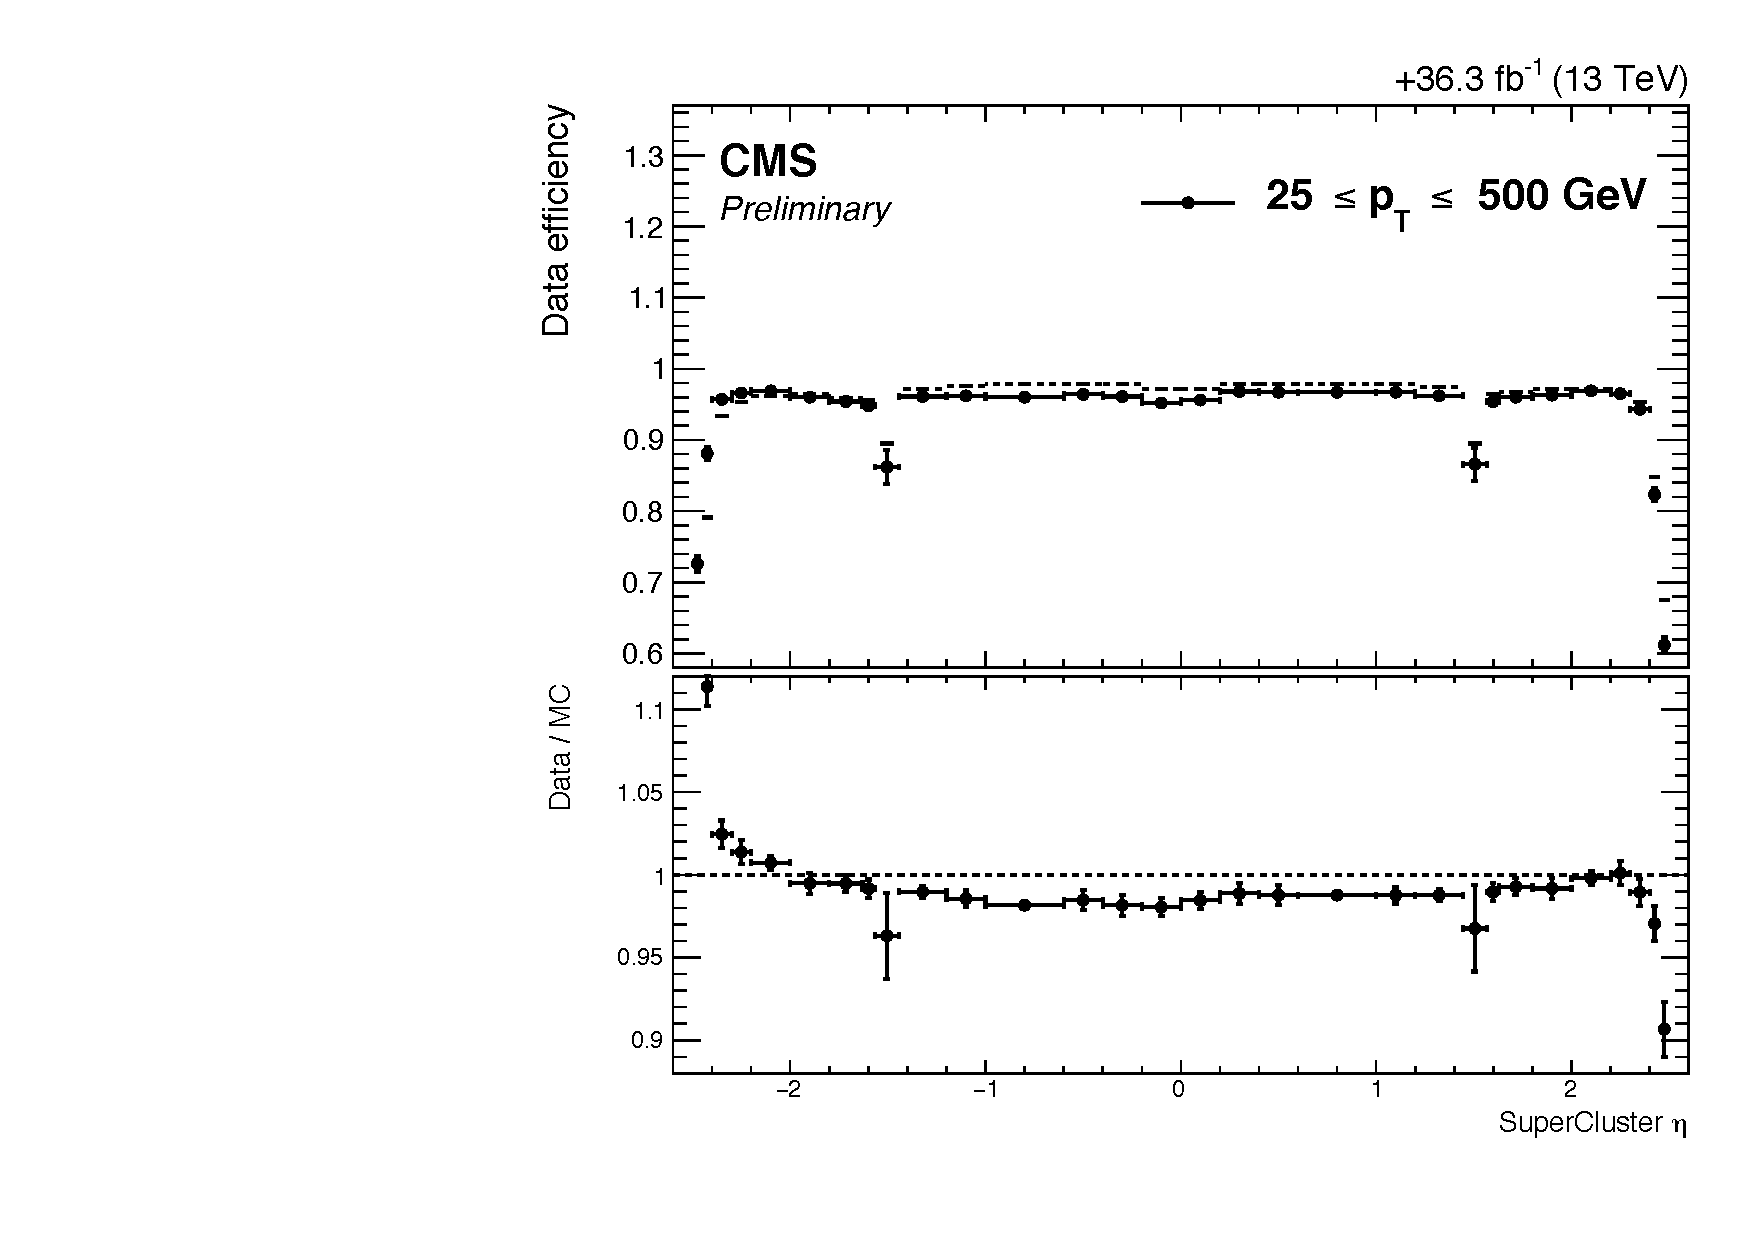
\includegraphics[width=0.7\textwidth]{Figures/Electrons/ele_rec_scale_factors.pdf}
\end{center}
\caption{Electron reconstruction efficiencies in data (top) and data to simulation scale factors (bottom).}
\label{fig:ele_rec_scale_factors}
\end{figure}

\subsection{Electron identification}
\label{sec:eleID}

Reconstructed electrons are identified by means of a Gradient Boosted Decision Tree (GBDT) multivariate classifier algorithm, which exploits observables from the EM cluster, the matching between the cluster and the electron track, as well as observables based exclusively on tracking measurements. 
The BDT has been retrained using CMSSW\_8\_0\_X samples. The classifier is trained on Drell-Yan plus jets MC sample for both signal and background.

%{
%\resizebox{\textwidth}{!}{%
%\tiny  
%/DYJetsToLL\_M-50\_TuneCUETP8M1\_13TeV-madgraphMLM-pythia8/RunIISpring16DR80-PUSpring16\_80X\_mcRun2\_asymptotic\_2016\_v3\_ext1-v1/
%}}
%{
%\tiny  
%\begin{verbatim}
%/DYJetsToLL_M-50_TuneCUETP8M1_13TeV-madgraphMLM-pythia8/RunIISpring16DR80-PUSpring16_80X_mcRun2_asymptotic_2016_v3_ext1-v1/
%\end{verbatim}
%}

The impact of the retraining of the ID for the 2016 conditions is illustrated in the receiver operating characteristic (ROC) curves shown in Figure~\ref{fig:ele_ID_ROC}. Several studies to improve the performance of the multivariate analysis (MVA) for the harsher 2016 running conditions were performed. 
One study considered a new splitting of the BDT training bins, where electrons falling into the gap regions of the ECAL, e.g. the EB-EE transition region, were trained separately from the non-gap electrons. 
However, no improvement for either population was observed, indicating that the current setup is already able to properly take the significantly differing input distributions in those regions into account. 
Additional variables were also studied, including more cluster-shape observables. 
Still, none of these variables helped to improve the performance in the relevant $>95\%$ signal efficiency regime, though up to a $20\%$ improved background rejection was seen for $80\%$ of working points. 
Finally, the hyperparameters of the MVA were systematically scanned for their optimal values, but the resulting configuration was found to improve the overall performance only marginally by $<10\%$ and introduced a significant overtraining effect. 
Due to the small gains and large overtraining, it was decided to not modify the hyperparameters beyond the interface changes from the latest 4.2.0 version of the TMVA package.

Figure~\ref{fig:ele_ID_BDT_output} shows the output of the BDT on the training and testing samples for true and fake electrons 
for the high-$p_T$ training bin in the end cap. 
The good agreement between the training and testing distributions is similar across the six training bins and indicates that the classifier has not been overtrained.

\begin{figure}[!htb]
\vspace*{0.3cm}
\begin{center}
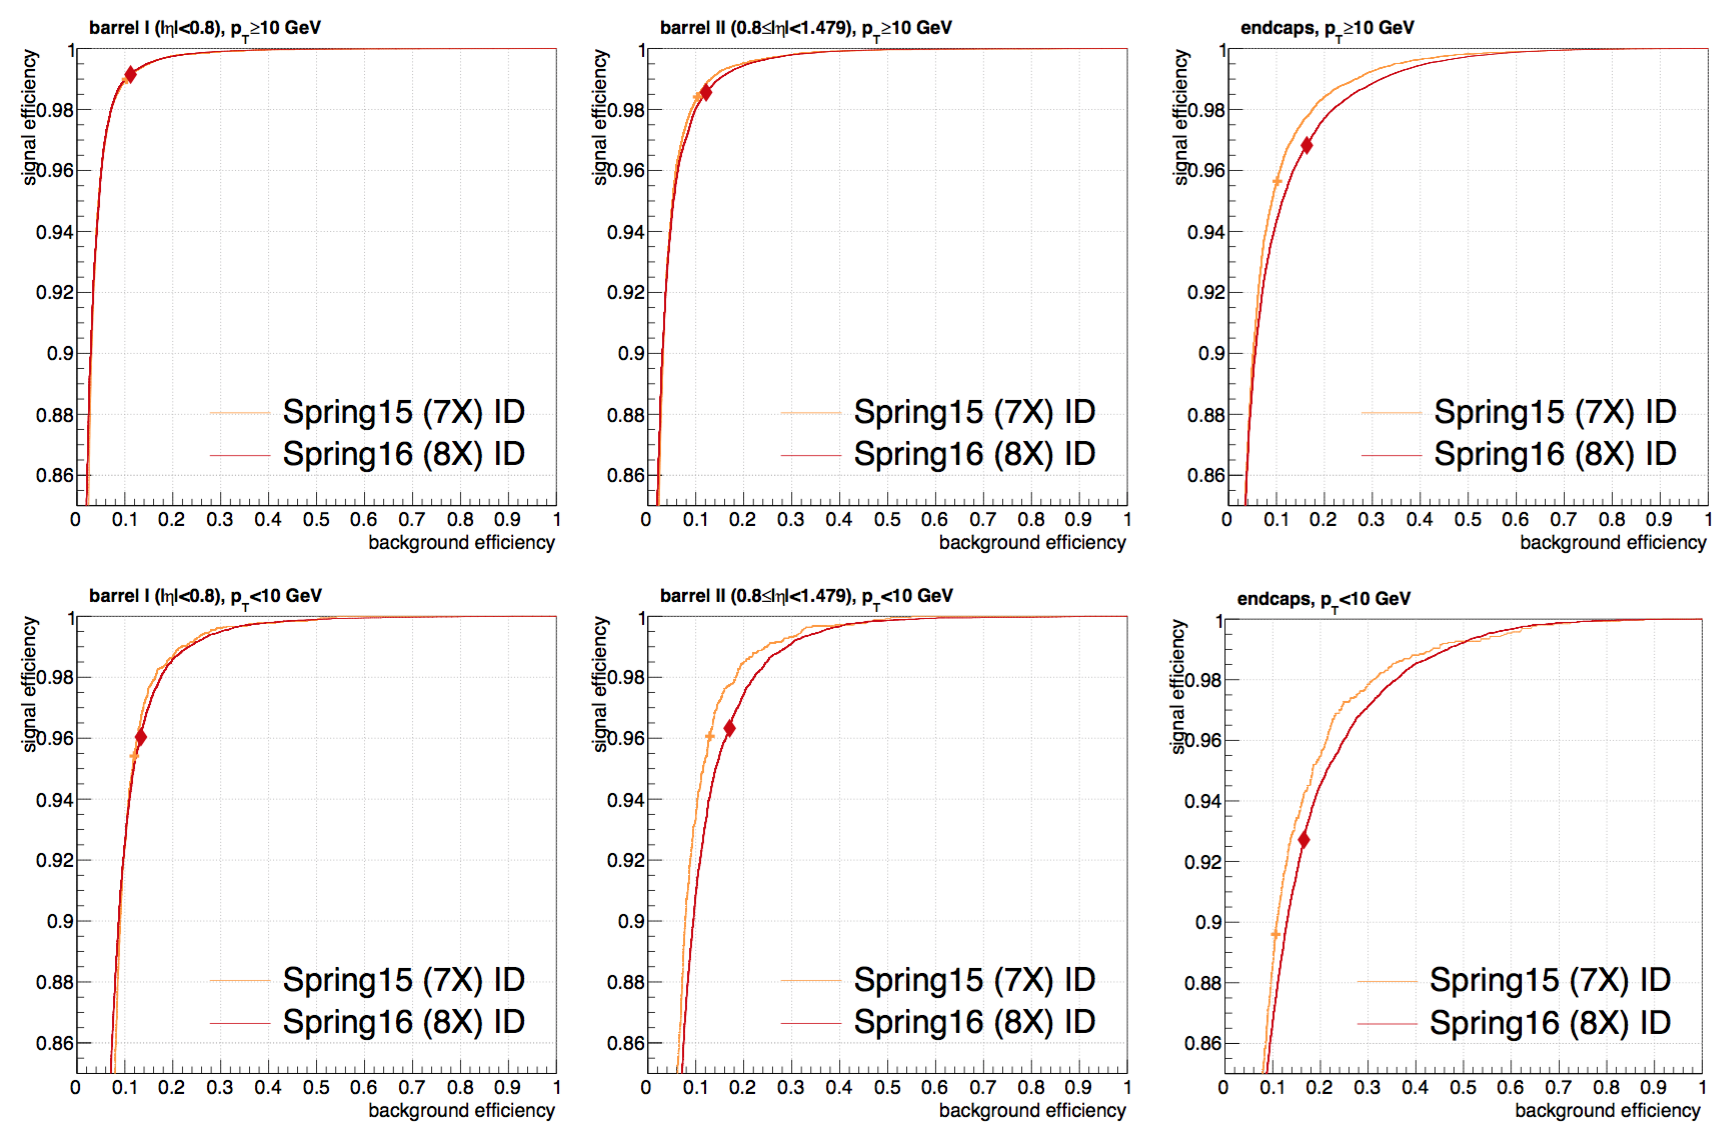
\includegraphics[width=0.9\textwidth]{Figures/Electrons/ele_ROC.png}
\caption{Performance comparison of the MVA trained for the 2015 analysis and the retraining for 2016 conditions. 
The respective working points are indicated by the markers.
\label{fig:ele_ID_ROC}}
\end{center}
\end{figure}

\begin{figure}[!htb]
\vspace*{0.3cm}
\begin{center}
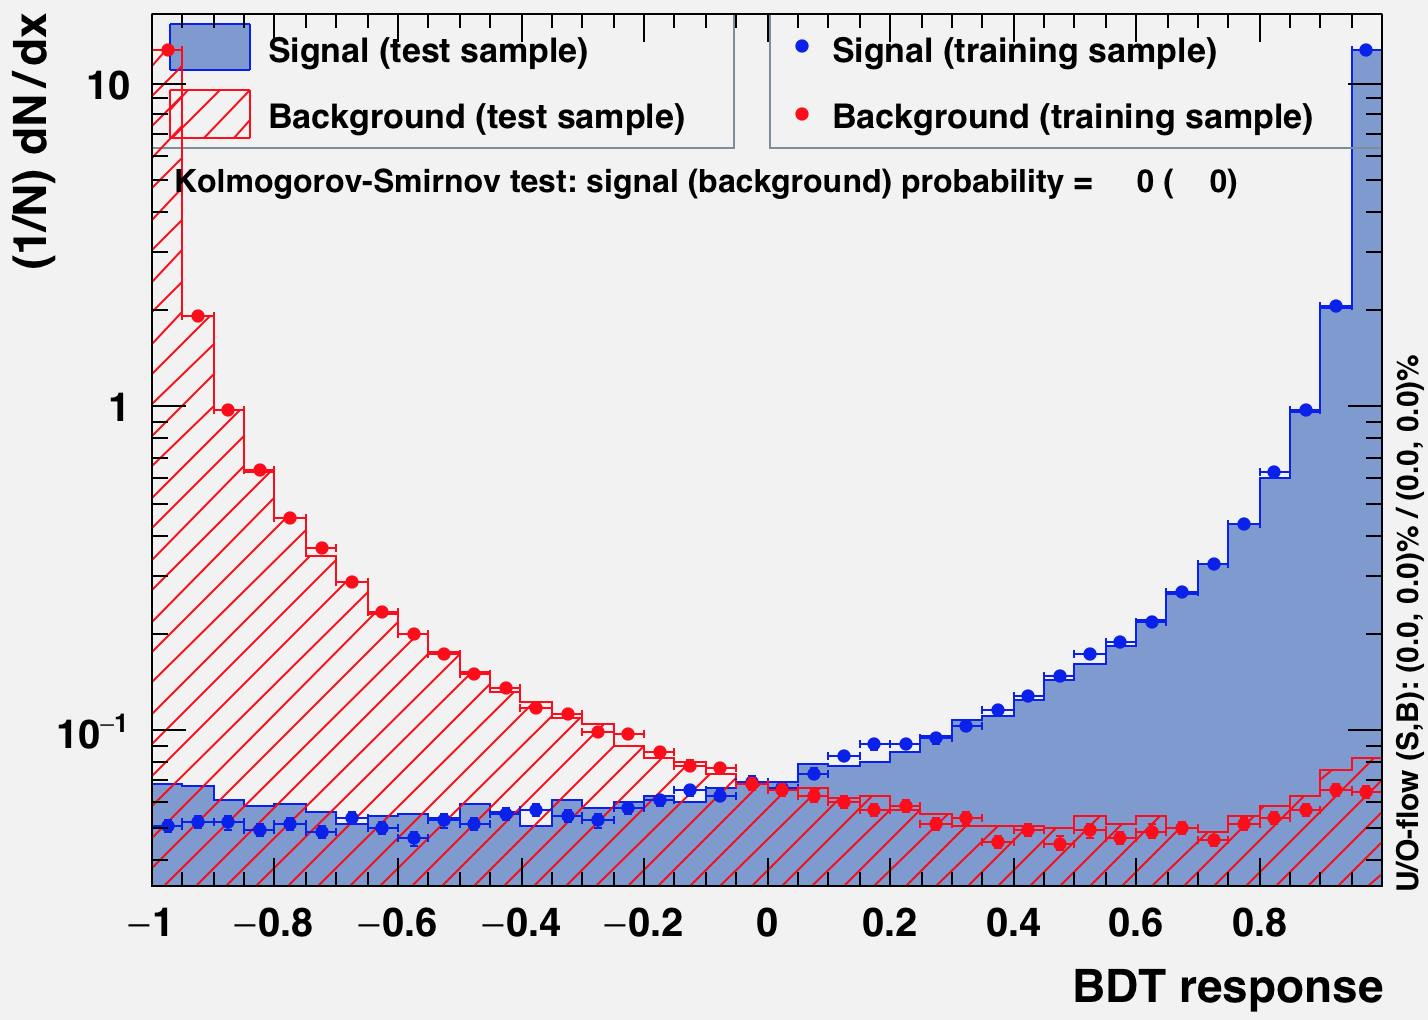
\includegraphics[width=0.7\textwidth]{Figures/Electrons/ele_overtraining.png}
\caption{Boosted decision tree output for the training and testing sample for true and fake electrons in the high-$p_T$ end cap training bins.
\label{fig:ele_ID_BDT_output}}
\end{center}
\end{figure}

Table~\ref{tab:ele_ID_input_variables} summarizes the full list of observables used as inputs to the classifier
and Table~\ref{tab:ele_ID_WP} lists the cut values applied to the BDT score for the chosen working point. 
For the analysis, we define "tight" electrons as the loose electrons that pass this MVA identification working point. 

 \begin{table}[h!]
\scriptsize
    \centering
\resizebox{\textwidth}{!}{%
    \begin{tabular}{c|l}
\hline %----------------------------------------------------------------------------------------
%\multicolumn{4}{|c|}{Datasets}                                                                \\
observable type    &  observable name      	\\
\hline %----------------------------------------------------------------------------------------

\multirow{6}{*}{cluster shape}
	&  RMS of the energy-crystal number spectrum along $\eta$ and $\varphi$; $\sigma_{i\eta i\eta}$, $\sigma_{i\varphi i\varphi}$		\\
	&  supercluster width along $\eta$ and $\phi$		\\
	&  'ratio of the hadronic energy behind the electron 
supercluster to the supercluster energy, $H/E$			\\
	&  circularity $(E_{5\times5} - E_{5\times1})/E_{5\times5}$			\\
	&  sum of the seed and adjacent crystal over the super cluster energy $R_{9}$			\\
	&  for end cap traing bins: energy fraction in preshower $E_{PS}/E_{raw}$			\\
\hline
\multirow{2}{*}{track-cluster matching}
	& energy-momentum agreement $E_{tot}/p_{in}$, $E_{ele}/p_{out}$, $1/E_{tot} - 1/p_{in}$ 			\\
	& position matching $\Delta\eta_{in}$, $\Delta\varphi_{in}$, $\Delta\eta_{seed}$			\\
\hline
\multirow{5}{*}{tracking}
        & fractional momentum loss $f_{brem} = 1 - p_{out}/p_{in}$	\\
        & number of hits of the KF and GSF track $N_{KF}$, $N_{GSF}$ $(\mathord{\cdot})$ \\
        & reduced $\chi^2$ of the KF and GSF track $\chi^{2}_{KF}$, $\chi^{2}_{\textrm{GSF}}$ \\
        & number of expected but missing inner hits $(\mathord{\cdot})$ 	\\
        & probability transform of conversion vertex fit $\chi^2$ $(\mathord{\cdot})$ \\

\hline %----------------------------------------------------------------------------------------
     \end{tabular}}
%\small
    \caption{Overview of input variables to the identification classifier. Variables not used in the Run 1 MVA are marked with  $(\mathord{\cdot})$.}
    \label{tab:ele_ID_input_variables}
\end{table}


\begin{table}[h!]
%\scriptsize
    \centering
    \begin{tabular}{c|c|c|c}
%\multicolumn{4}{|c|}{Datasets}                                                                \\
\hline %----------------------------------------------------------------------------------------
minimum BDT score    &  $|\eta| < 0.8 $ & $0.8 < |\eta| < 1.479$ 	& $|\eta| > 1.479$      \\
\hline %----------------------------------------------------------------------------------------
$ 5 < p_T < 10 $ $\GeV$ &  -0.211      & -0.396  		& -0.215		\\
$p_T > 10$ $\GeV$       &  -0.870		& -0.838		& -0.763		\\
\hline %----------------------------------------------------------------------------------------
     \end{tabular}
%\small
    \caption{Minimum boosted decision tree score required for passing the electron identification.}
    \label{tab:ele_ID_WP}
\end{table}


\subsection{Electron isolation}
\label{sec:eleiso}

The relative isolation for electrons is defined as: 

\begin{equation}
\text{RelPFiso} = (\sum_{\text{charged}} p_T + \sum^{\text{corr}}_{\text{neutral}} p_T)/p_T^{\text{lepton}}  
\label{eqn:elepfrelisoeqn}
\end{equation} 
where the corrected neutral component of isolation is computed using the formula:

\begin{equation}
\label{eqn:neutralea}
  \sum^{\text{corr}}_{\text{neutral}} p_T = \text{max}(\sum^{\text{uncorr}}_{\text{neutral}} p_T - \rho \times A_\text{eff},0 \GeV)  
\end{equation}
and the mean pileup contribution to the isolation cone is obtained as:  

\begin{equation}
 PU =  \rho \times A_\text{eff}
\label{eqn:purho}
\end{equation}
where $\rho$ is the mean energy density in the event, and the effective area $A_{eff}$ is defined as the ratio
between the slope of the average isolation and that of $\rho$ as a function of the number of vertices. 

The electron isolation working point was optimized and chosen to be $\text{RelPFiso}(\Delta R = 0.3) < 0.35$ \cite{AN-15-277}. 


\subsection{Electron energy calibrations}

Electrons in data are corrected for features in ECAL energy scale
in bins of $\pt$ and $\left| \eta \right|$. Corrections are calculated
on a $\cPZ \to \Pe\Pe$ sample to align the dielectron 
mass spectrum in the data to that in the MC and to
minimize its width.

The $\cPZ \to \Pe\Pe$ mass resolution in MC is made to match
data by applying a pseudorandom Gaussian smearing to electron energies,
with Gaussian parameters varying in bins of $\pt$ and $\left| \eta \right|$.
This has the effect of convoluting the electron energy spectrum with a
Gaussian.

The electron energy scale is measured in data by fitting a Crystal-Ball function to the dielectron mass spectrum around the $Z$ peak in the $Z+\ell$ control region. 
The energy scale for the full 2016 dataset is shown in Figure~\ref{fig:ele_energy_scale}(a) and agrees with the MC with 100 $\MeV$. 
The stability of the energy scale across different run periods is shown in Fig.~\ref{fig:ele_energy_scale}(b), where the data is binned into approximately 500~pb luminosity blocks.

%\begin{figure}[!htb]
%\vspace*{0.3cm}
%\begin{center}
%\subfigure [] {\resizebox{7.5cm}{!}{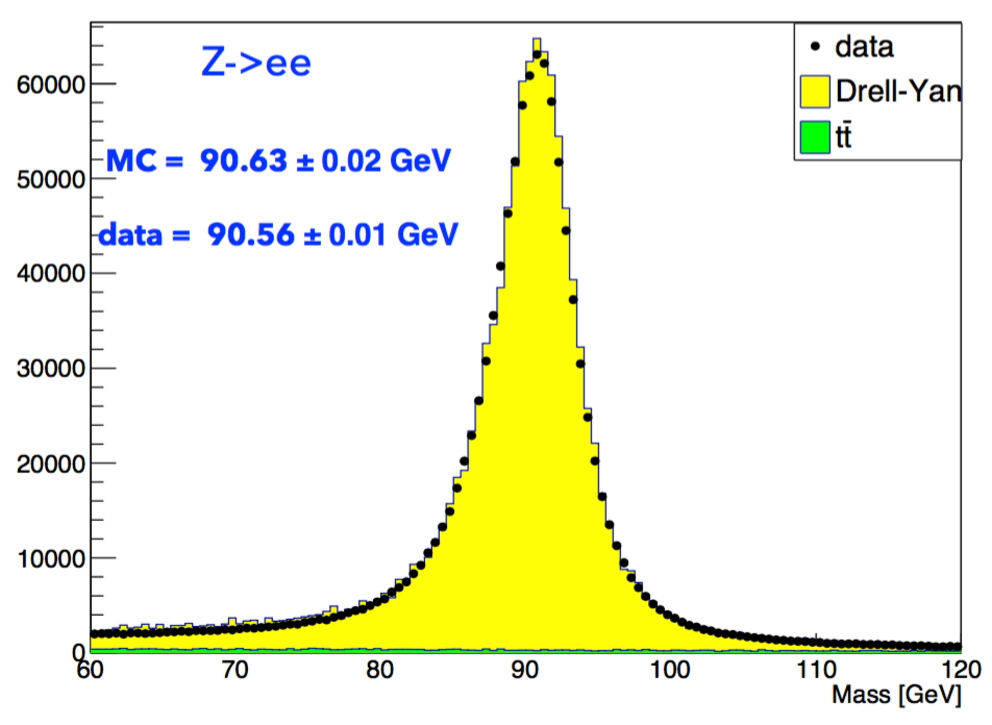
\includegraphics{Figures/Electrons/ele_energy_scale.pdf}}}
%\subfigure [] {\resizebox{9.5cm}{!}{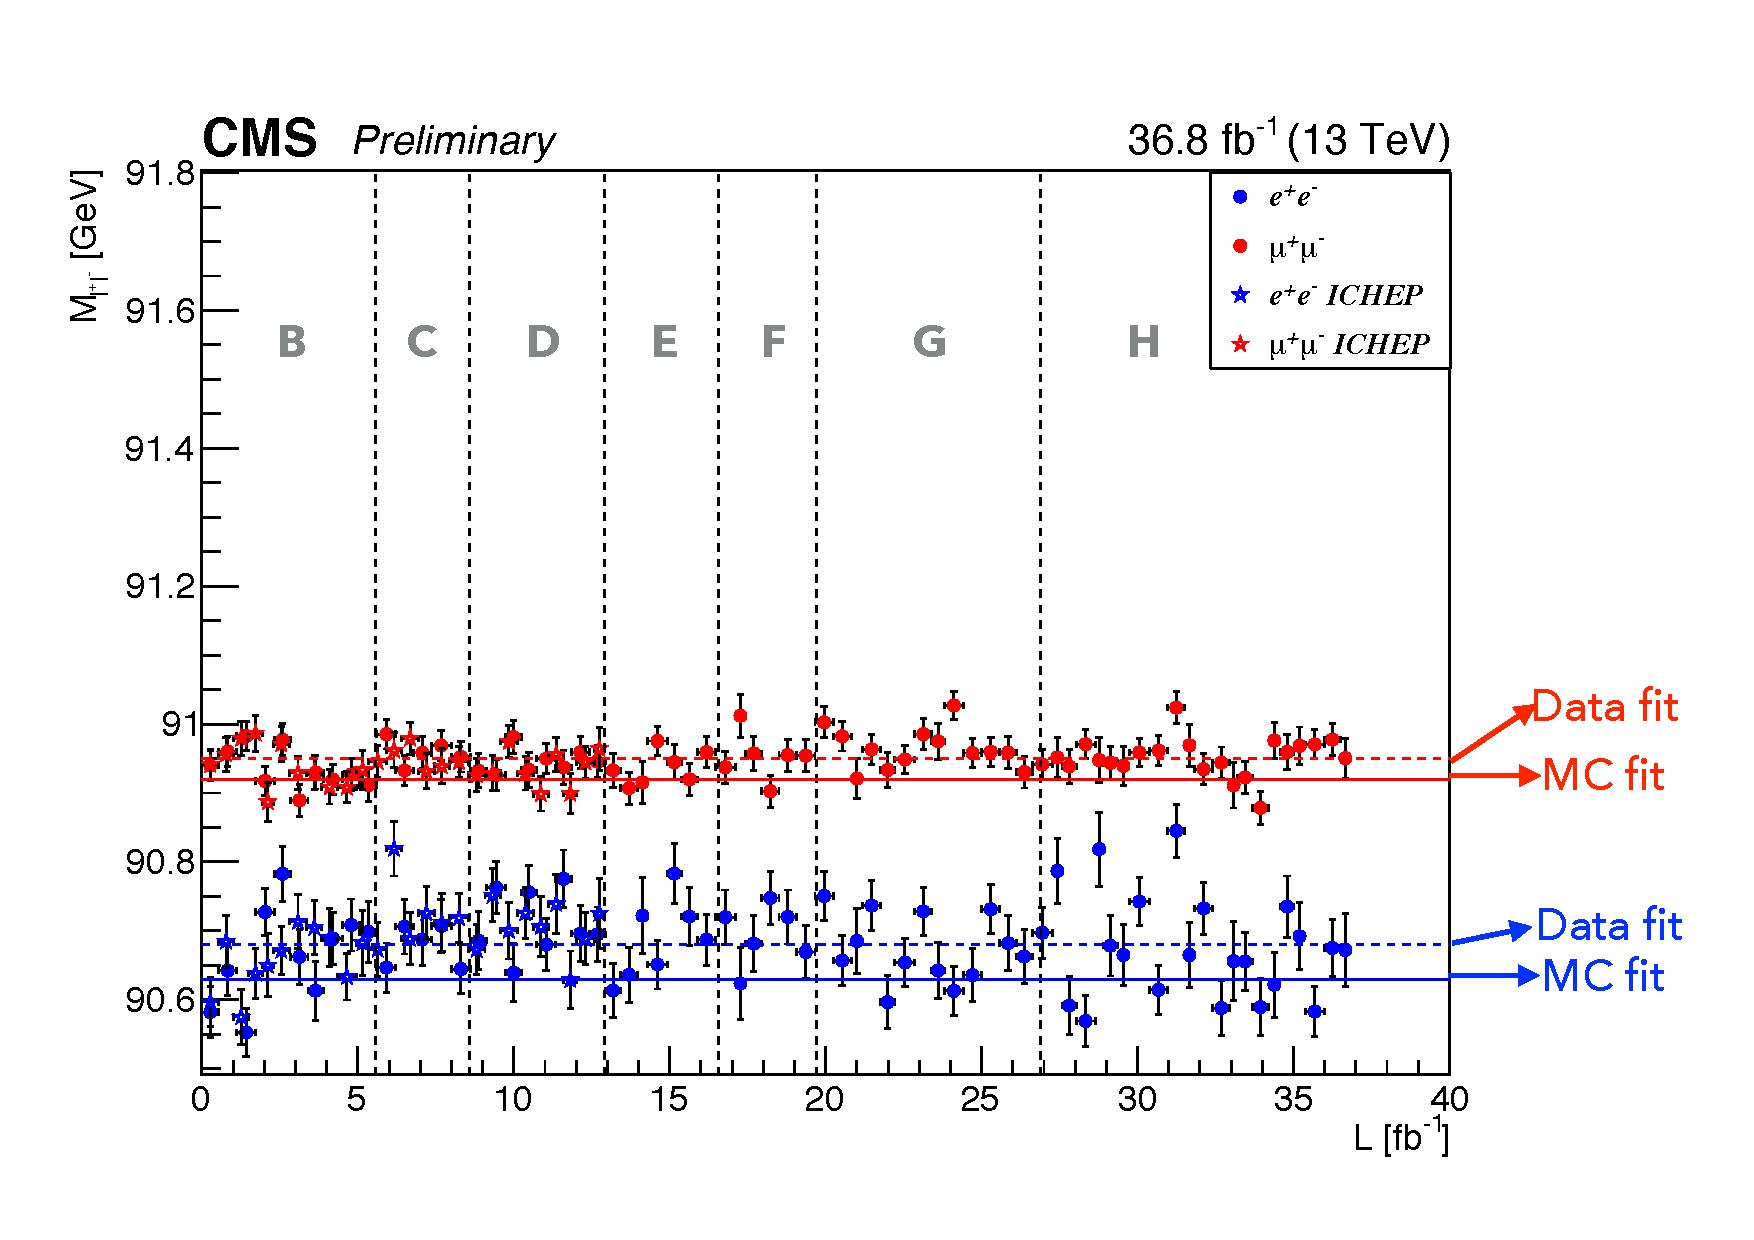
\includegraphics{Figures/Electrons/ele_energy_scale_per_lumi.pdf}}}
%\end{center}
%\caption{
%(a): electron energy scale measured in the $Z+\ell$ control region for EB and EE electrons. The results of the Crystall-ball fit are reported in the figure. 
%(b): lepton energy scales per 500~pb luminosity block. 
%}
%\label{fig:ele_energy_scale}
%\end{figure}

\begin{figure}[tbh]
\centering
\begin{subfigure}{0.9\textwidth}
\centering
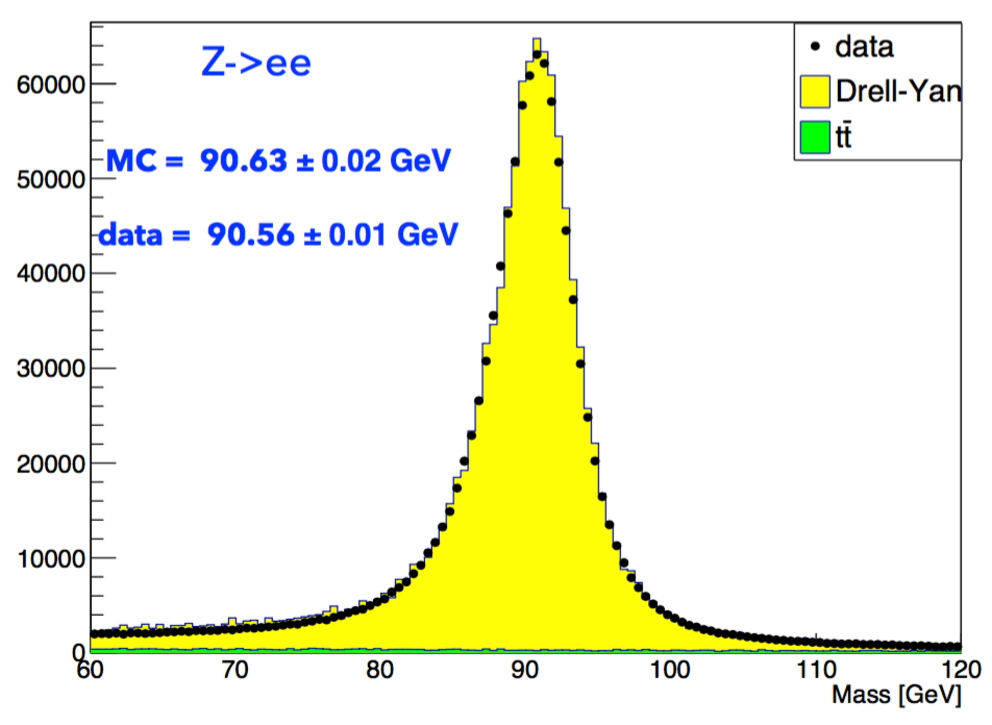
\includegraphics[width=4in]{Figures/Electrons/ele_energy_scale.pdf}
\caption{}
\end{subfigure}
\begin{subfigure}{0.9\textwidth}
\centering
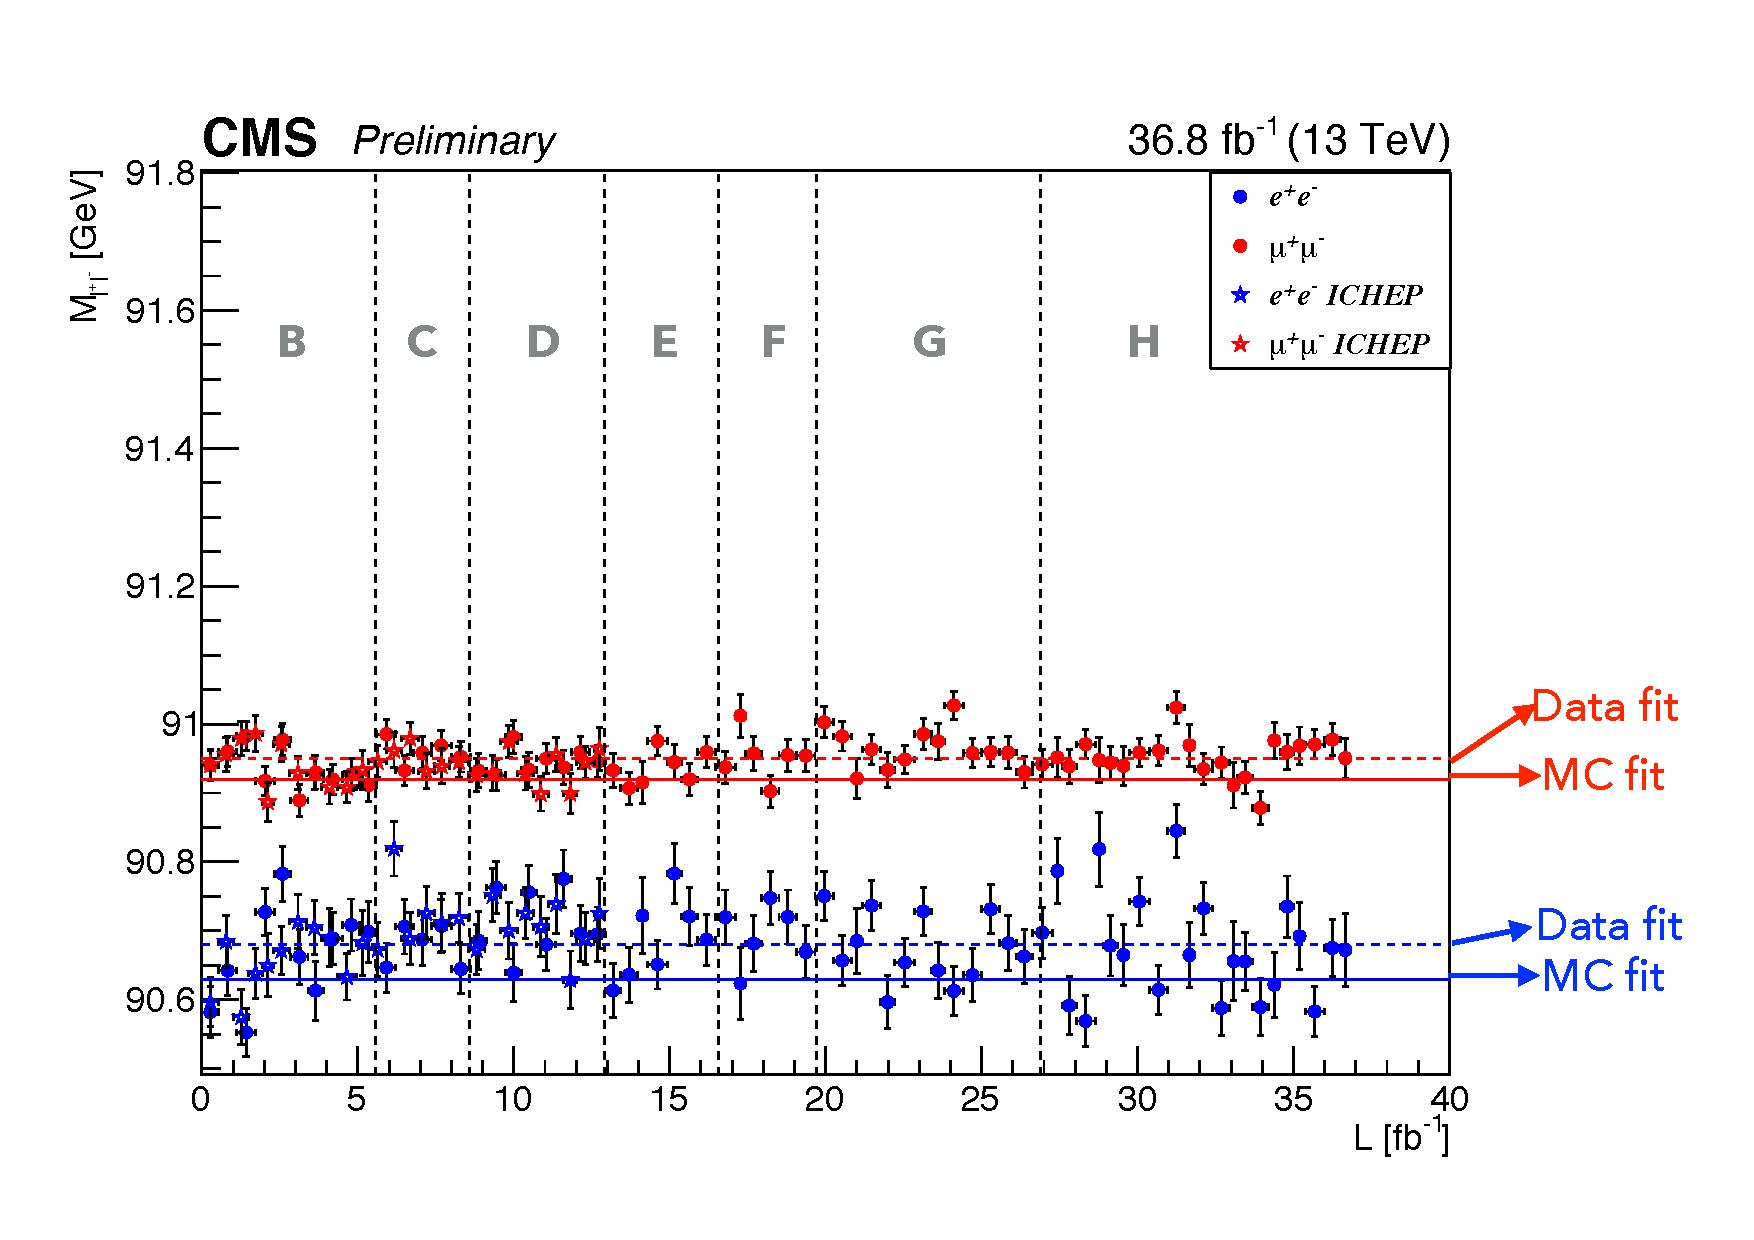
\includegraphics[width=4.5in]{Figures/Electrons/ele_energy_scale_per_lumi.pdf}
\caption{}
\end{subfigure}
\caption{(a): Electron energy scale measured in the $Z+\ell$ control region for EB and EE electrons. The results of the Crystall-ball fit are reported in the figure. (b): lepton energy scales per 500~pb luminosity block.}
\label{fig:ele_energy_scale}
\end{figure}

\subsection{Electron efficiency measurements}
\label{sec:eleEffMeas}
%\input{Objects/eleEffMeas.tex}

The tag-and-probe (T\&P) study was performed on the single electron primary datasets listed in Table~\ref{tab:datasets_data} using the same golden JSON of 36.8 
fb$^{-1}$ as for the main analysis \cite{AN-15-277}. 

Tag electrons need to satisfy the following quality requirements:
(1) trigger matched to HLT\_Ele27\_eta2p1\_WPTight\_Gsf\_v*
(2) $p_{T} > 30$ $\GeV$, super cluster (SC) $\eta < 2.1$ but on in EB-EE gap ($1.4442<|\eta|<1.566$)
and (3) tight working point of the Spring16 cut-based electron ID.

Probe electrons only need to be reconstructed as GsfElectron, electrons associated with a GsfTrack object. The FSR recovery algorithm used in the main analysis is used consistently throughout the efficiency measurement; the isolations are calculated without any FSR photons matched to electrons and the probe electron $\pt$ as well as the dielectron invariant mass include the FSR photons, if any. 


The nominal MC efficiencies are evaluated from the LO MadGraph Drell-Yan sample, while the NLO systematics use the 0,1 jet MadGraph\_AMCatNLO sample listed in Table \ref{tab:MCsamples}.

In contrast to previous efficiency measurements, a template fit is used here. The $m_{ee}$ signal shape of the passing and failing probes is taken from MC and convoluted with a Gaussian. The data is then fitted with the convoluted MC template and a CMSShape, an error function with a one-sided exponential tail. This change follows from the usage of the new T\&P tool developed by the EGM POG.


%\paragraph{Electron selection efficiency measurements}\mbox{}\\
%\label{par:Efficiency_measurements}

The electron selection efficiency is measured as a function of the probe electron $\pt$ and its SC $\eta$, and separately for electrons falling in the ECAL gaps. Figure \ref{fig:ele_sel_pt_turn_on} shows the $\pt$ turn-on curves measured in data, and the final two-dimensional scale factor is shown in Figure~\ref{fig:ele_sel_scale_factors} together with the systematic uncertainties. These scale factors are very similar to the ICHEP figures, except more homogenous across $\eta$ and $\pt$ because of the higher statistics and the usage of more stable fitting routines in the new T\&P tool.


%\begin{figure}[!htb]
%\begin{center}
%    \subfigure [] {\resizebox{7.5cm}{!}{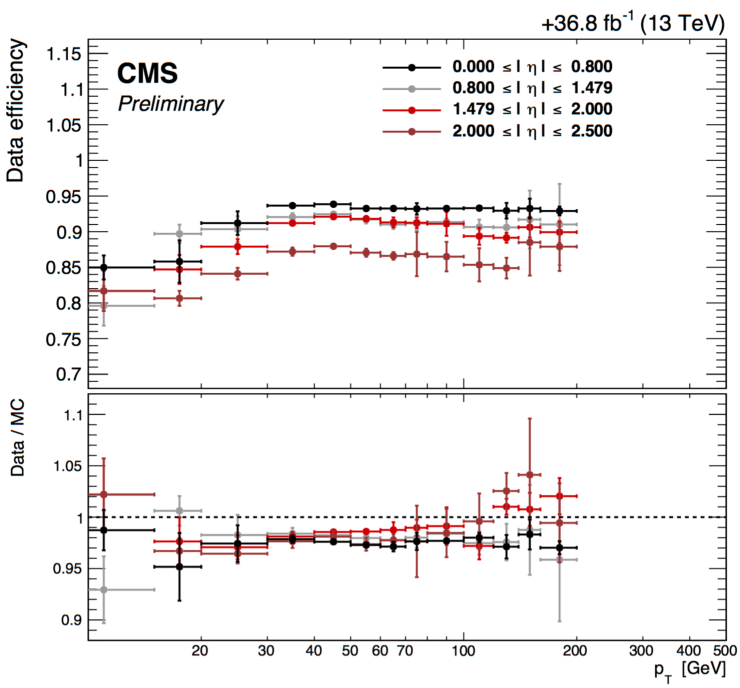
\includegraphics{Figures/Electrons/ele_eff_pt.pdf}}}
%    \subfigure [] {\resizebox{7.5cm}{!}{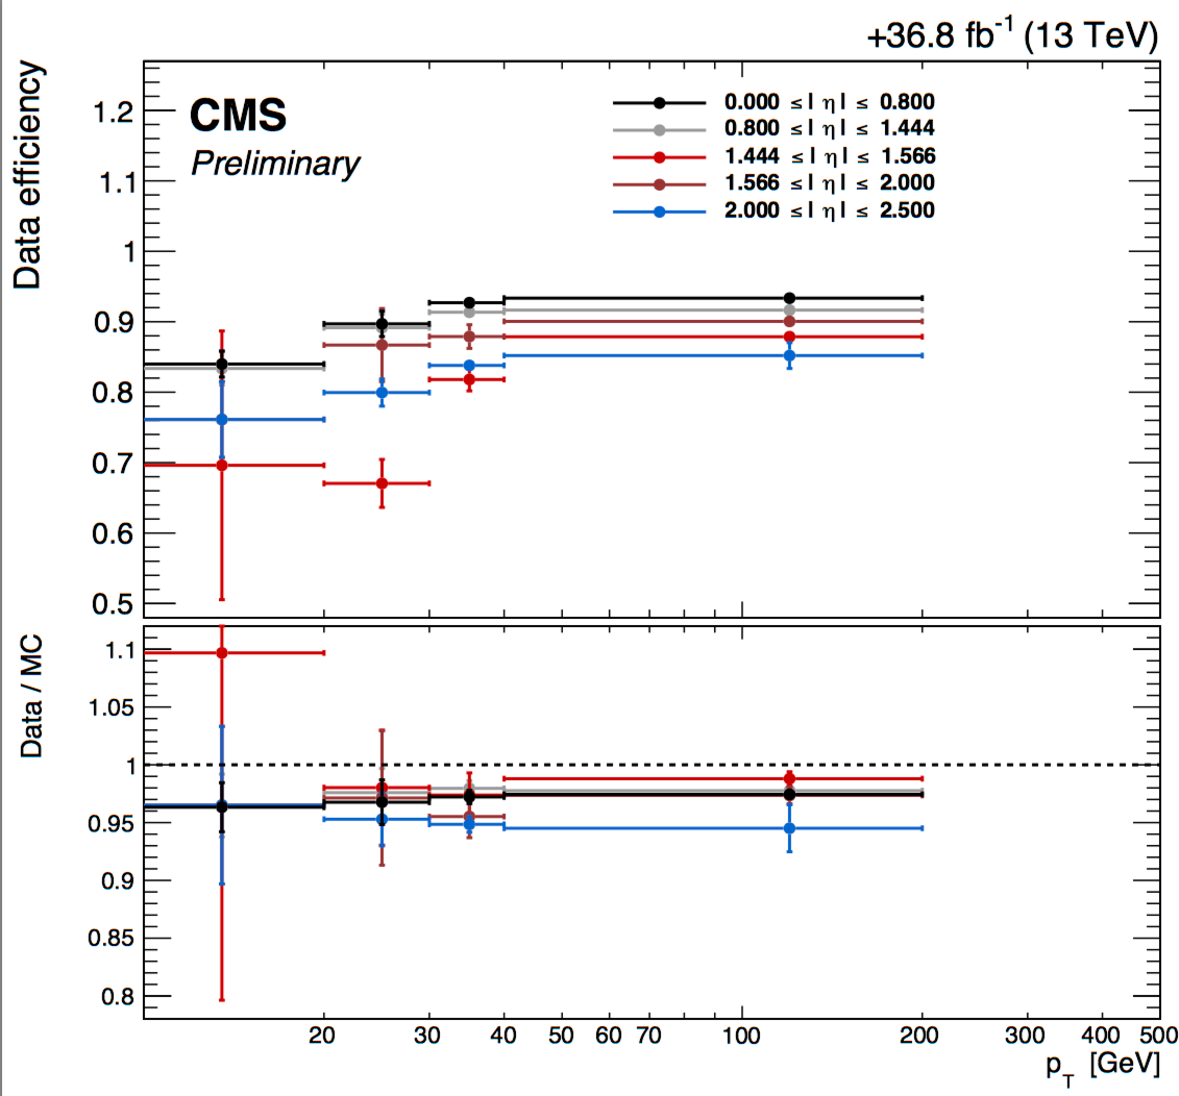
\includegraphics{Figures/Electrons/gap_ele_eff_pt.pdf}}}\\
%\caption{Electron selection efficiencies measured using the Tag-and-Probe technique described in the text, non-gap electrons (left) and gap electrons (right).}
%\label{fig:ele_sel_pt_turn_on}
%\end{center}
%\end{figure}

\begin{figure}[tbh]
\centering
\begin{subfigure}{0.95\textwidth}
\centering
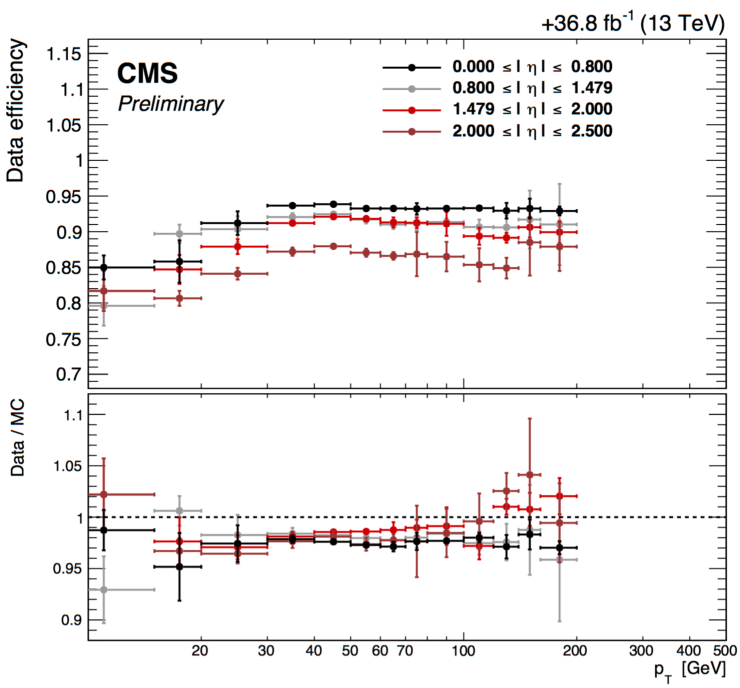
\includegraphics[width=3.5in]{Figures/Electrons/ele_eff_pt.pdf}
\caption{}
\end{subfigure}
\begin{subfigure}{0.95\textwidth}
\centering
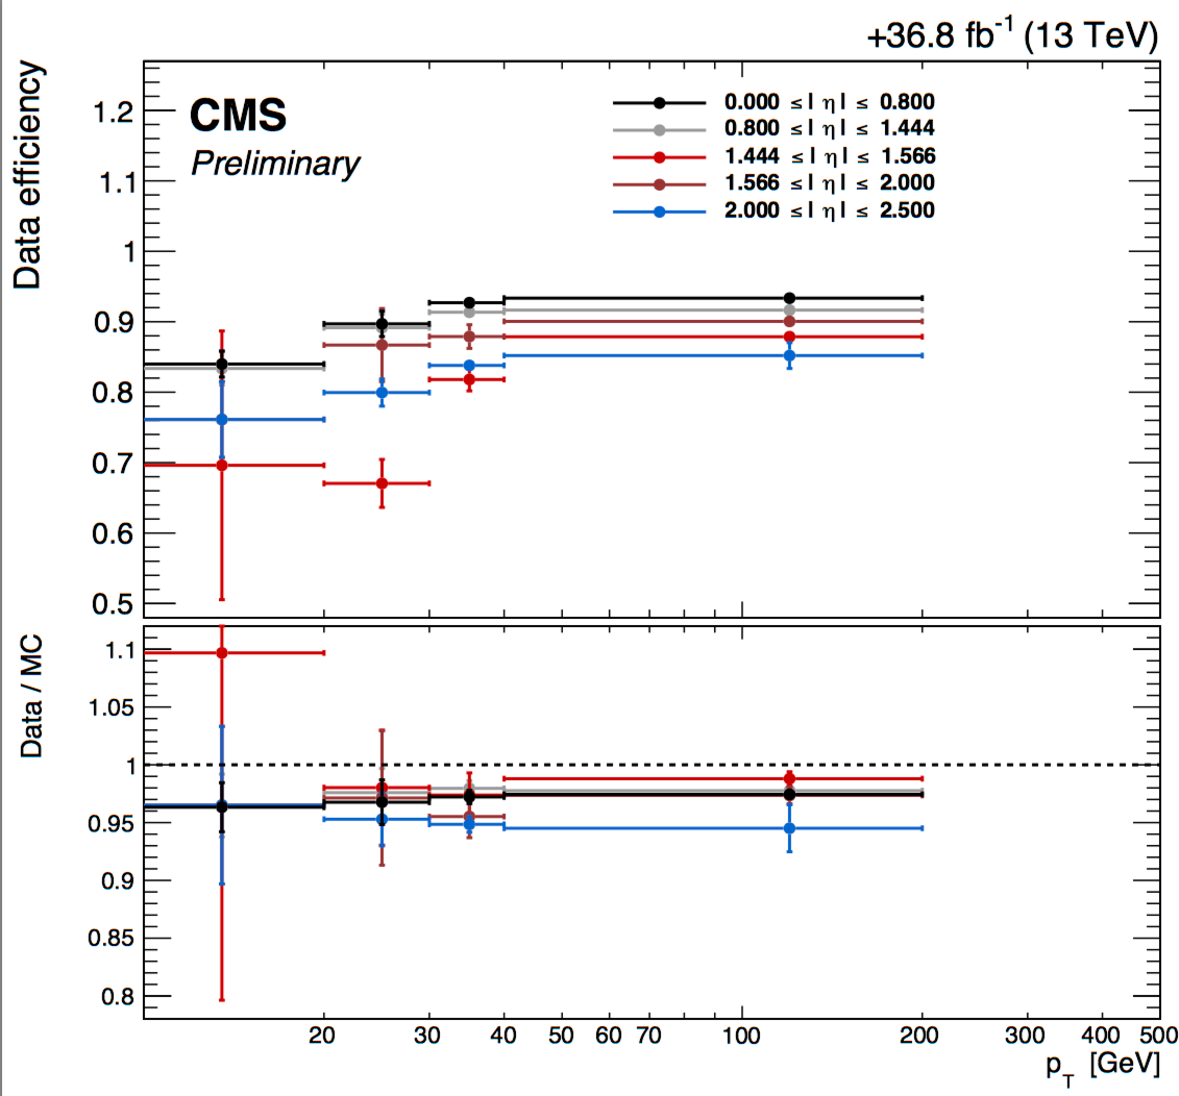
\includegraphics[width=3.5in]{Figures/Electrons/gap_ele_eff_pt.pdf}
\caption{}
\end{subfigure}
\caption{Electron selection efficiencies measured using the tag-and-probe technique described in the text, non-gap electrons (a) and gap electrons (b).}
\label{fig:ele_sel_pt_turn_on}
\end{figure}

%\begin{figure}[!htb]
%\begin{center}
%    \subfigure [] {\resizebox{15cm}{!}{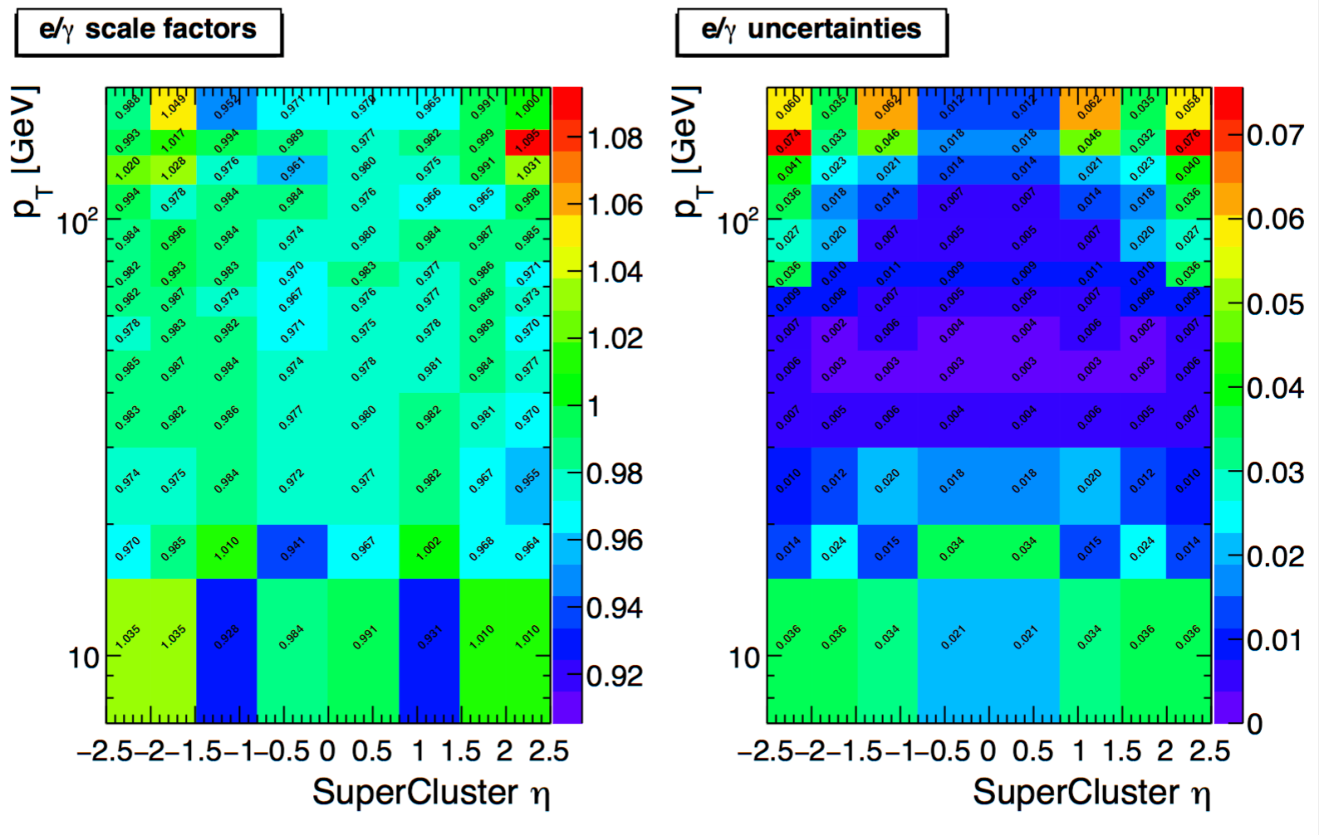
\includegraphics{Figures/Electrons/ele_eff_sf_unc.pdf}}}\\
%    \subfigure [] {\resizebox{15cm}{!}{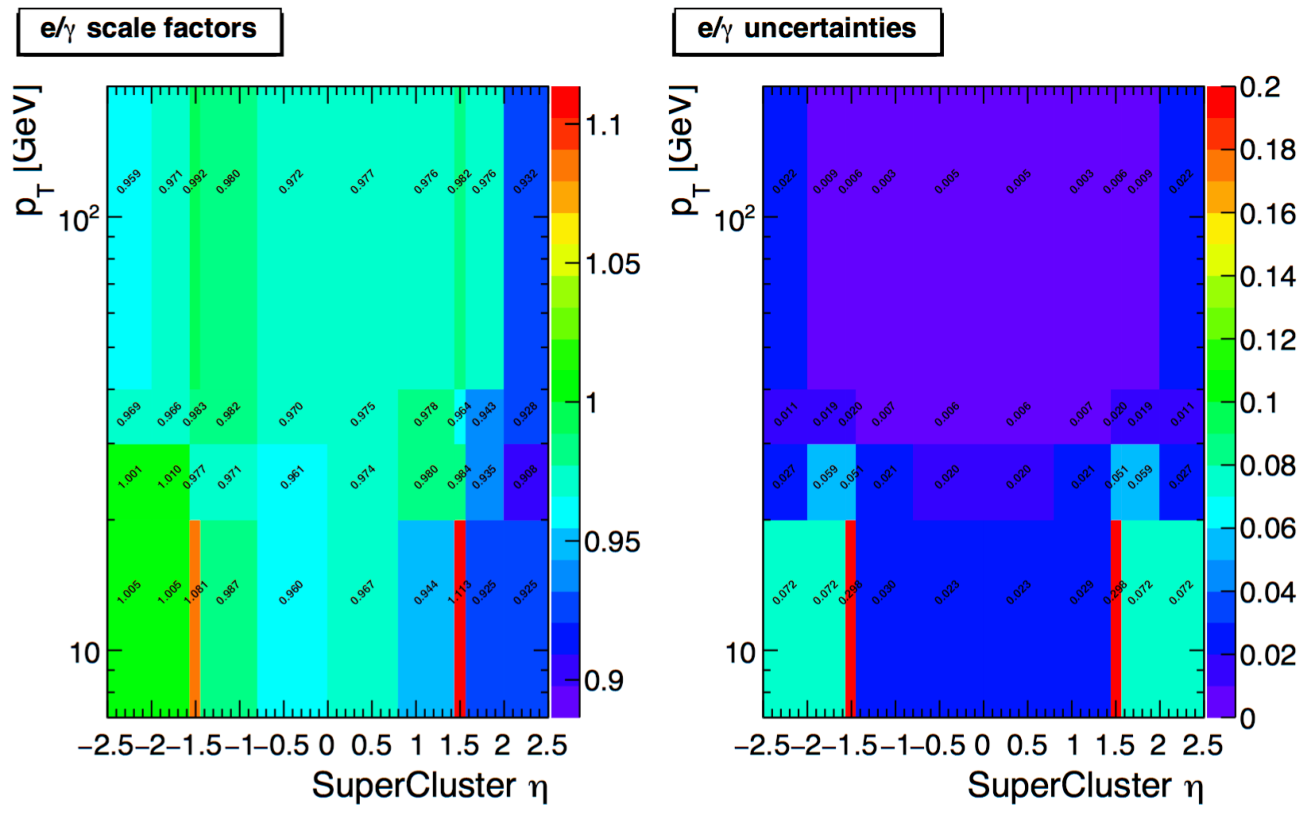
\includegraphics{Figures/Electrons/gap_ele_eff_sf_unc.pdf}}}
%\caption{Electron selection efficiencies measured using the Tag-and-Probe technique described in the text, non-gap electrons (top) and gap electrons (bottom).}
%\label{fig:ele_sel_scale_factors}
%\end{center}
%\end{figure}

\begin{figure}[tbh]
\centering
\begin{subfigure}{0.95\textwidth}
\centering
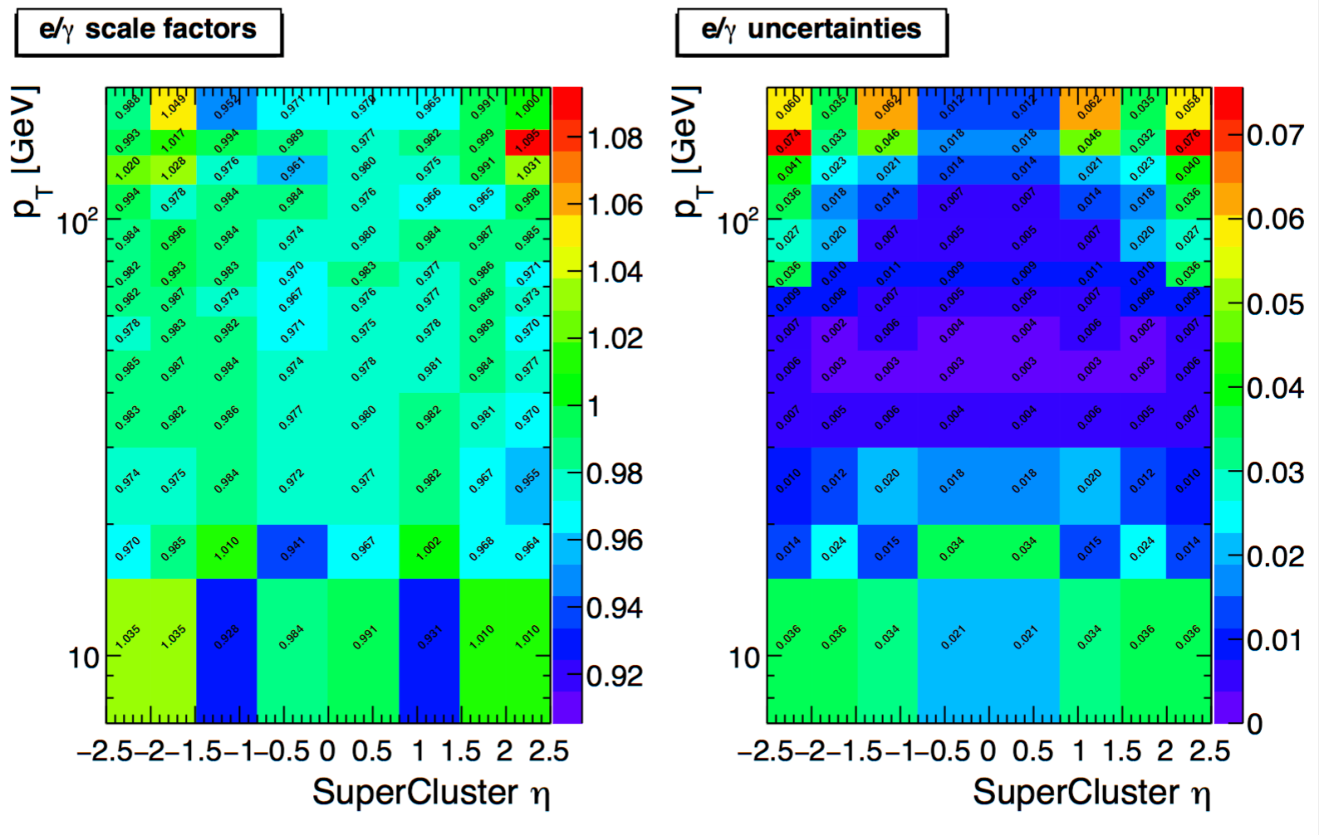
\includegraphics[width=5in]{Figures/Electrons/ele_eff_sf_unc.pdf}
\caption{}
\end{subfigure}
\begin{subfigure}{0.95\textwidth}
\centering
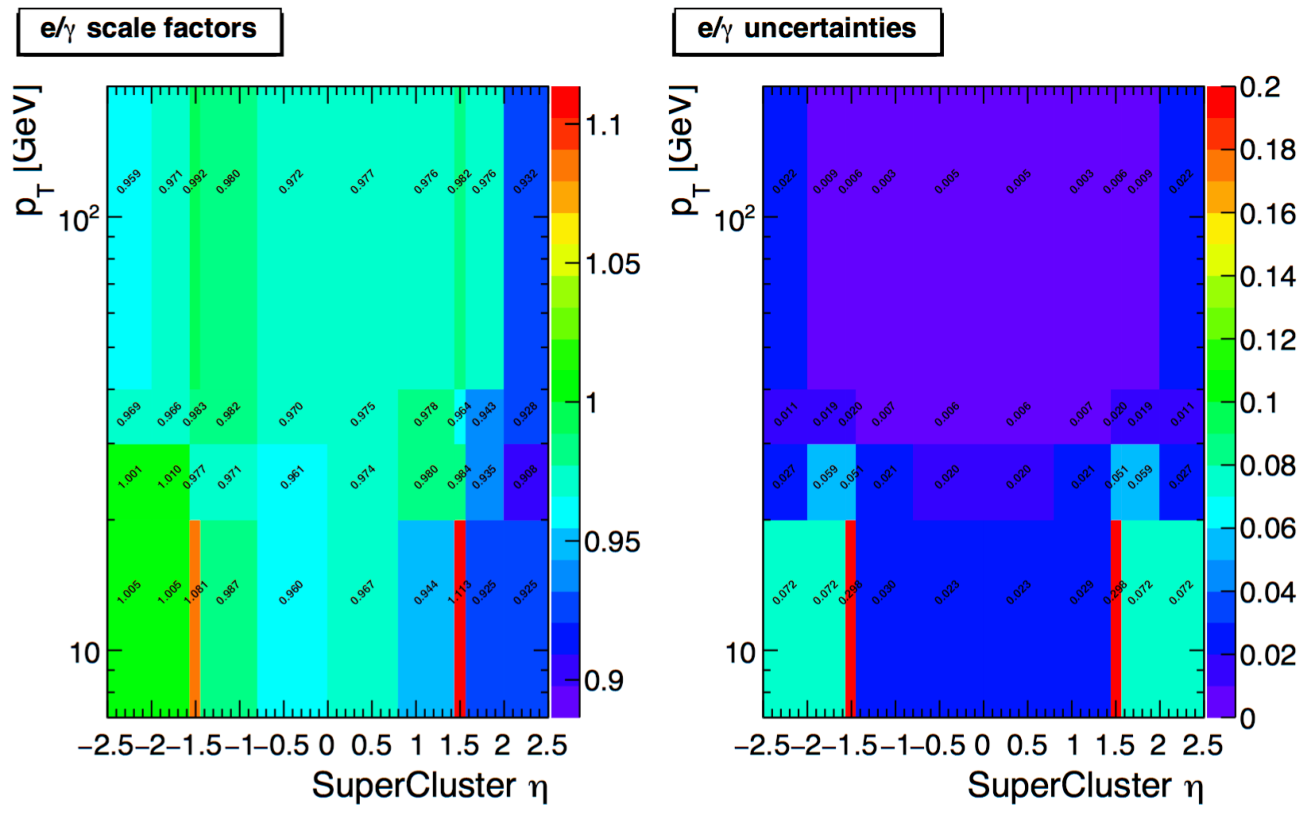
\includegraphics[width=5in]{Figures/Electrons/gap_ele_eff_sf_unc.pdf}
\caption{}
\end{subfigure}
\caption{Electron selection efficiencies measured using the tag-and-probe technique described in the text, non-gap electrons (a) and gap electrons (b)}
\label{fig:ele_sel_scale_factors}
\end{figure}


%\paragraph{Systematic uncertainties}\mbox{}\\
%\label{par:Systematic_uncertainties}
%%%%%%%%%%%%%%%%%%%%%%%%%%%%

The EGM recommendations on the evaluation of T\&P uncertainties for efficiency measurements are followed. Specifically: 
(1) Variation of the signal shape from a MC shape to an analytic shape (Crystal-Ball) fitted to the MC
(2) Variation of the background shape from a CMS-shape to a simple exponential in fits to data
(3) Variation of the tag selection: tag $p_{T}>$35 $\GeV$ and passes MVA-based ID, and
(4) Using an NLO MC sample for the signal templates.
The total uncertainty for the measurement of the scale factors is the quadratic sum of the statistical uncertainties returned from the fit and the aforementioned systematic uncertainties.


\section{Muons}

\subsection{Muon reconstruction and identification}
\label{sec:muonReco}

More details on muon reconstruction can be found in Ref.~\cite{AN-15-277}.
"Loose" muons are the muons that satisfy  
$p_T > 5$, $|\eta| < 2.4$, $d_{xy}< 0.5$, and $d_z < 1$, where $d_{xy}$ and $d_z$ are 
defined with respect to the primary vertex and using the muonBestTrack. Muons have to be 
reconstructed by either the Global Muon or Tracker Muon algorithm. Standalone 
muon tracks that are only reconstructed in the muon system are rejected.
Sstandalone muons are discarded even if they are marked as global or tracker muons. 

Loose muons with $\pt$ below 200 $\GeV$ are considered "tight" muons if they 
also pass the PF muon ID. Note that the naming 
convention used for these IDs differs from the muon POG naming scheme, in which
the ``tight ID'' used here is called the ``loose ID''. Loose muons with $\pt$ 
above 200 $\GeV$ are considered tight muons if they pass the PF ID or the Tracker
High-$\pt$ ID, the definition of which is shown in Table~\ref{tab:highPtID}.
This relaxed definition is used to increase signal efficiency for the high-mass
search. When a very heavy resonance decays to two $\cPZ$ bosons, both bosons
will be very boosted. In the laboratory frame, the leptons coming from the decay of
a highly boosted $\cPZ$ will be nearly collinear, and the PF ID loses 
efficiency for muons separated by approximately $\Delta R < 0.4$, which roughly 
corresponds to muons originating from $\cPZ$ bosons with $\pt > 500\ \GeV$.

\begin{table}[h]
    \begin{small}
    \begin{center}
    \begin{tabular}{l|l}
      \hline
      Plain-text description         & Technical description                 \\
      \hline
      Muon station matching          & Muon is matched to segments           \\
                                     & in at least two muon stations         \\
      %\hline                                                          
      Good $\pt$ measurement         & $\frac{\pt}{\sigma_{\pt}} < 0.3$      \\
      %\hline
      Vertex compatibility ($x-y$)   & $d_{xy} < 2$~mm                       \\
      %\hline
      Vertex compatibility ($z$)     & $d_{z} < 5$~mm                        \\
      %\hline
      Pixel hits                     & At least one pixel hit                \\
      %\hline
      Tracker hits                   & Hits in at least six tracker layers   \\
      \hline
    \end{tabular}
    \caption{
      The requirements for a muon to pass the Tracker High-$\pt$ ID. Note that
      these are equivalent to the Muon POG High-$\pt$ ID with the global track 
      requirements removed.
      }
    \label{tab:highPtID}
    \end{center}
    \end{small}
\end{table}

An additional ``ghost-cleaning'' step is performed to deal with situations when a single muon
can be incorrectly reconstructed as two or more muons. In this step, Tracker Muons that are not Global Muons are required to be arbitrated, and if two muons are sharing 50\% or more of their segments, then the muon with lower quality is removed.

\subsection{Muon isolation}
\label{sec:muoniso}

PF-based isolation, described for electrons in Section~\ref{sec:eleiso}, is also used for the muons. 
The only difference is the way the pileup contribution is subtracted; for the muons, $\Delta\beta$ correction is applied, whereby $\Delta\beta = \frac{1}{2} \sum^\text{charged had.}_\text{PU} \pt$  gives an estimate of the energy deposit of neutral particles (i.e. hadrons and photons) from pileup vertices. 
The relative isolation for muons is then defined as:
\begin{equation}
\text{RelPFiso} = \frac{\sum^\text{charged had.} \pt + \max(\sum^\text{neutral had.} \ET 
+ \sum^\text{photon} \ET - \Delta \beta, 0)}{\pt^\text{lepton}}
\label{eqn:mupfiso}
\end{equation}

The isolation working point for muons was optimized and chosen to be the same as for electrons, $\text{RelPFiso}(\Delta R = 0.3) < 0.35$ \cite{AN-15-277}. 

%\subsection{Muon Energy Calibrations}
% \input{Objects/muCalib}

\subsection{Muon efficiency measurements}
\label{sec:muonEffMeas}

Muon efficiencies are measured with the T\&P method performed on
$\cPZ \to \Pgm\Pgm$ and $\JPsi\to\mu\mu$ events in bins of $\pt$ and $\eta$ \cite{AN-15-277}.
The $\Z$ sample is used to measure the muon reconstruction and identification efficiency at high $\pt$
and the efficiency of the isolation and impact parameter requirements at all $\pt$.
The $\JPsi$ sample is used to measure the reconstruction efficiency at low $\pt$,
as it benefits from a better purity in that kinematic regime. In this case,
events are collected using HLT\_Mu7p5\_Track2\_Jpsi\_v* when probing the
reconstruction and identification efficiency in the muon system and using the
 HLT\_Mu7p5\_L2Mu2\_Jpsi\_v* when probing the tracking efficiency.

\subsubsection{Reconstruction and identification}

Results for the muon reconstruction and identification efficiency for $\pt > 20\ \GeV$
have been derived by the Muon POG.
The probe in this measurement are tracks reconstructed in the inner tracker, and
the passing probes are those that are also reconstructed as a global or tracker muon 
and passing the Muon POG Loose muon identification.
%
Results for low $\pt$ muons were derived using $\JPsi$ events, with the same definitions
of probe and passing probes. The systematic uncertainties are estimated by varying the analytical signal and background shape models used to fit 
the dimuon invariant mass \cite{AN-15-277}. The efficiency and scale 
factors used for low $\pt$ muons are the ones derived using single muon prompt-reco dataset.
The efficiency in data and simulation is shown in Figure~\ref{fig:MuonIDEff_1}. 

\begin{figure}[tbh]
\centering
\begin{subfigure}{0.3\textwidth}
\centering
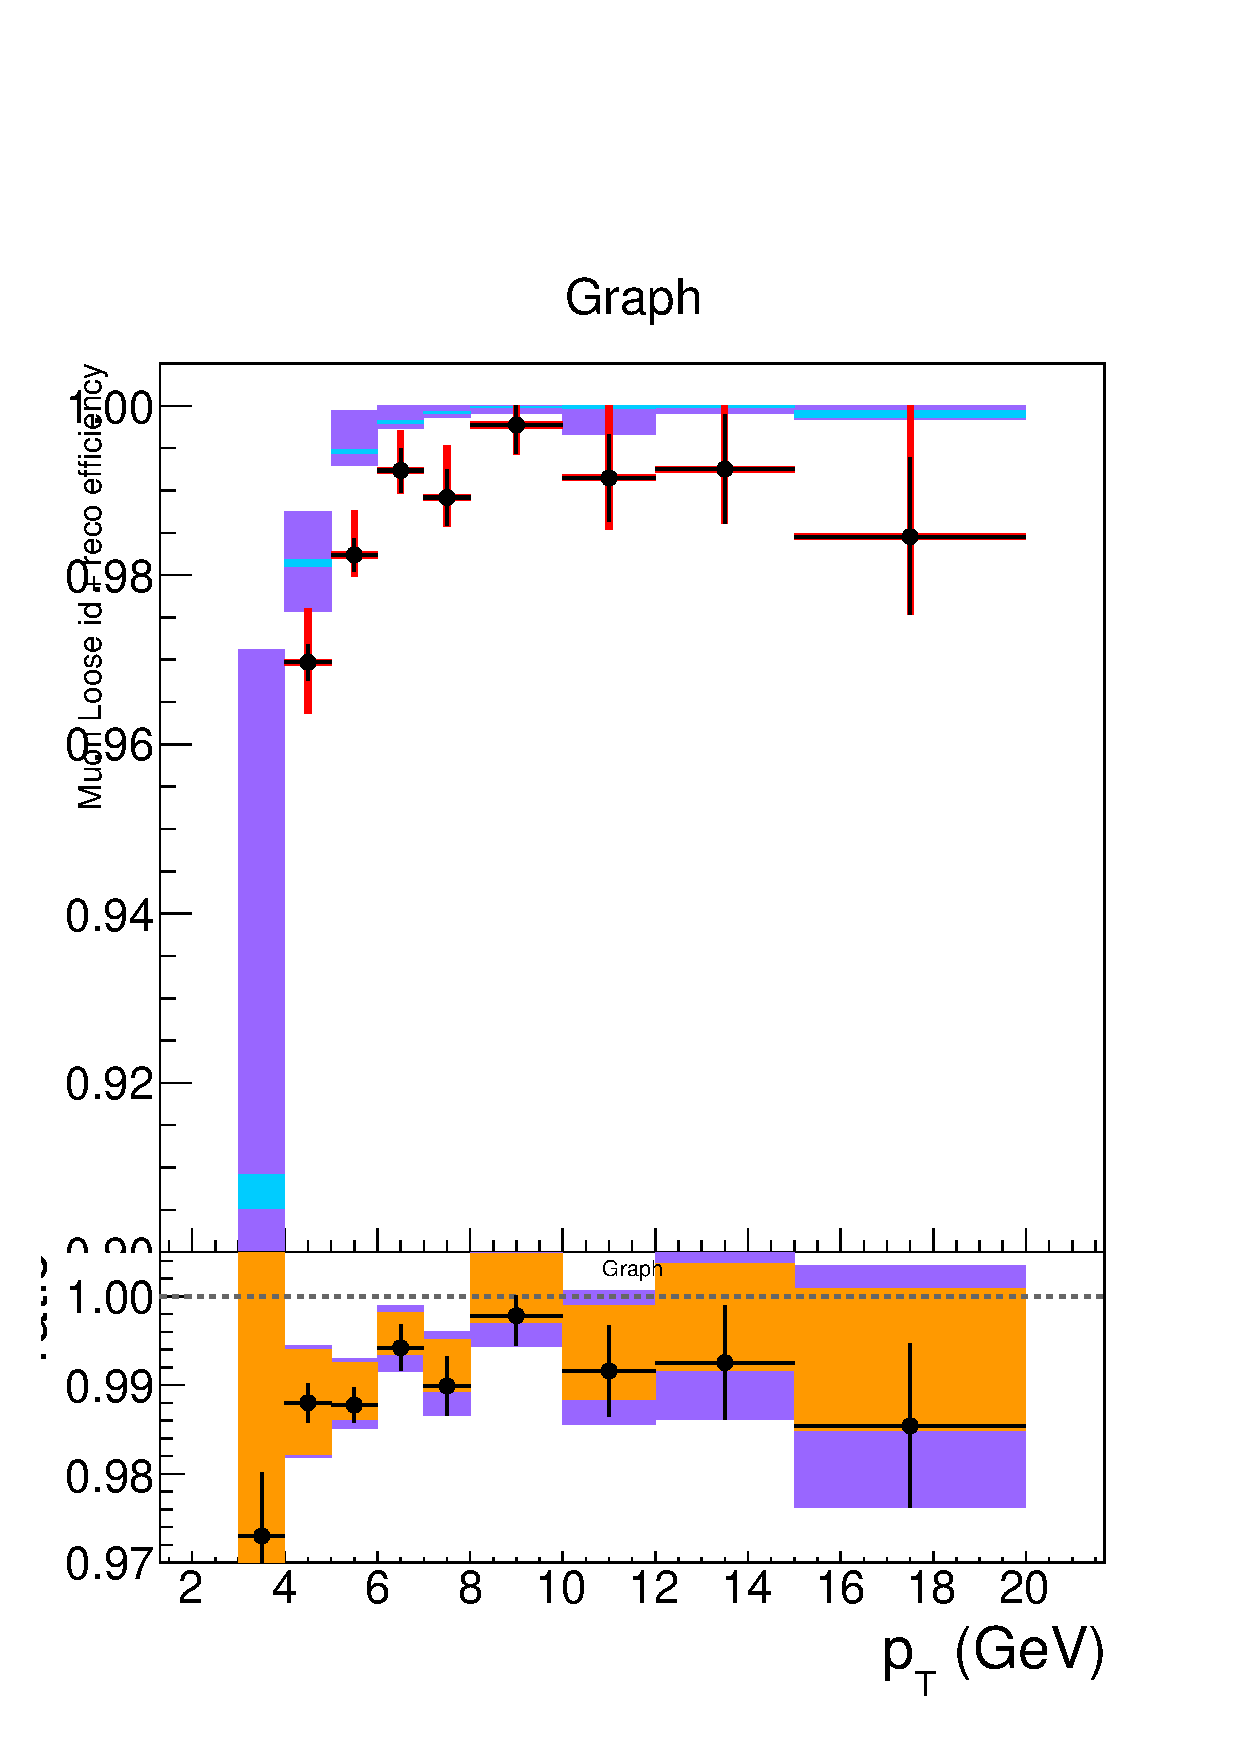
\includegraphics[width=2in]{Figures/Muons/mu_Loose_barrel.pdf}
\caption{}
\end{subfigure}
\begin{subfigure}{0.3\textwidth}
\centering
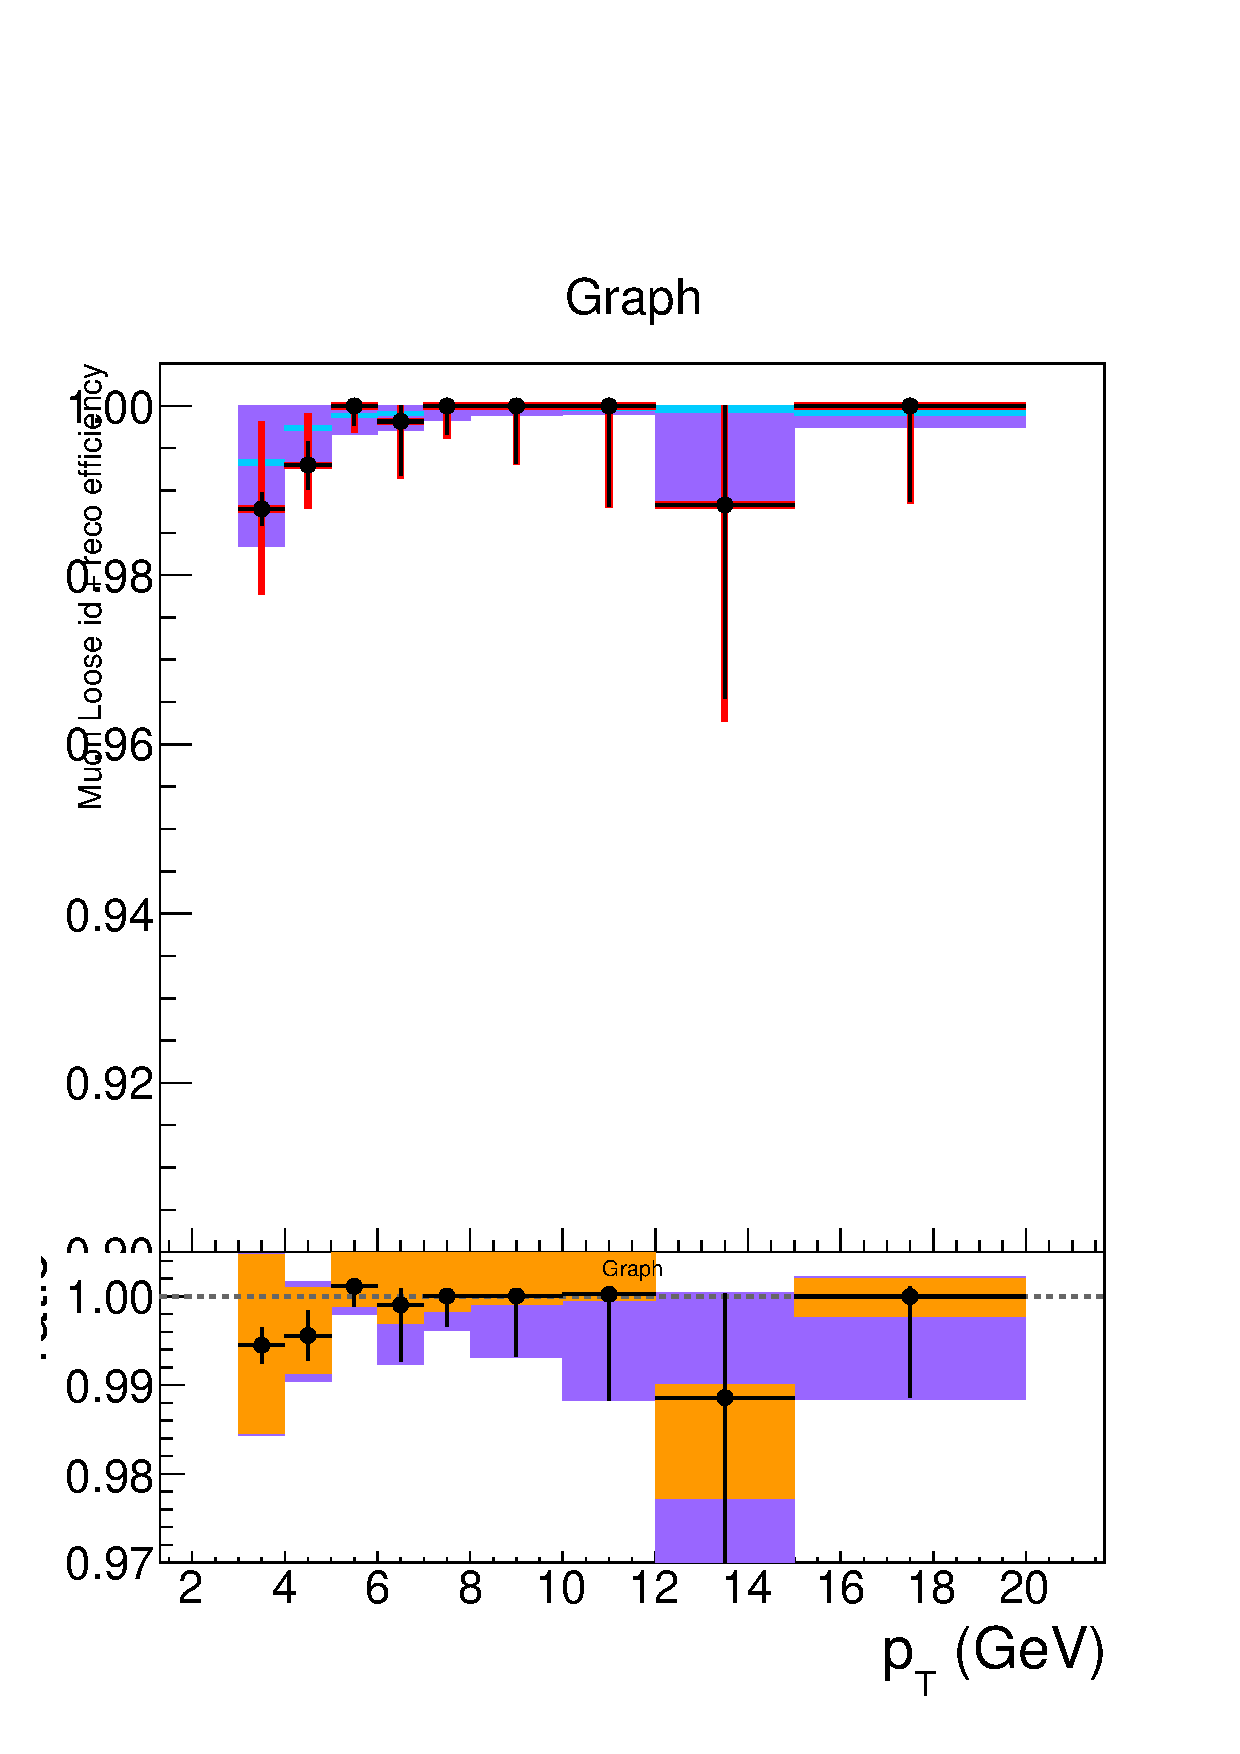
\includegraphics[width=2in]{Figures/Muons/mu_Loose_endcap.pdf}
\caption{}
\end{subfigure}
\begin{subfigure}{0.3\textwidth}
\centering
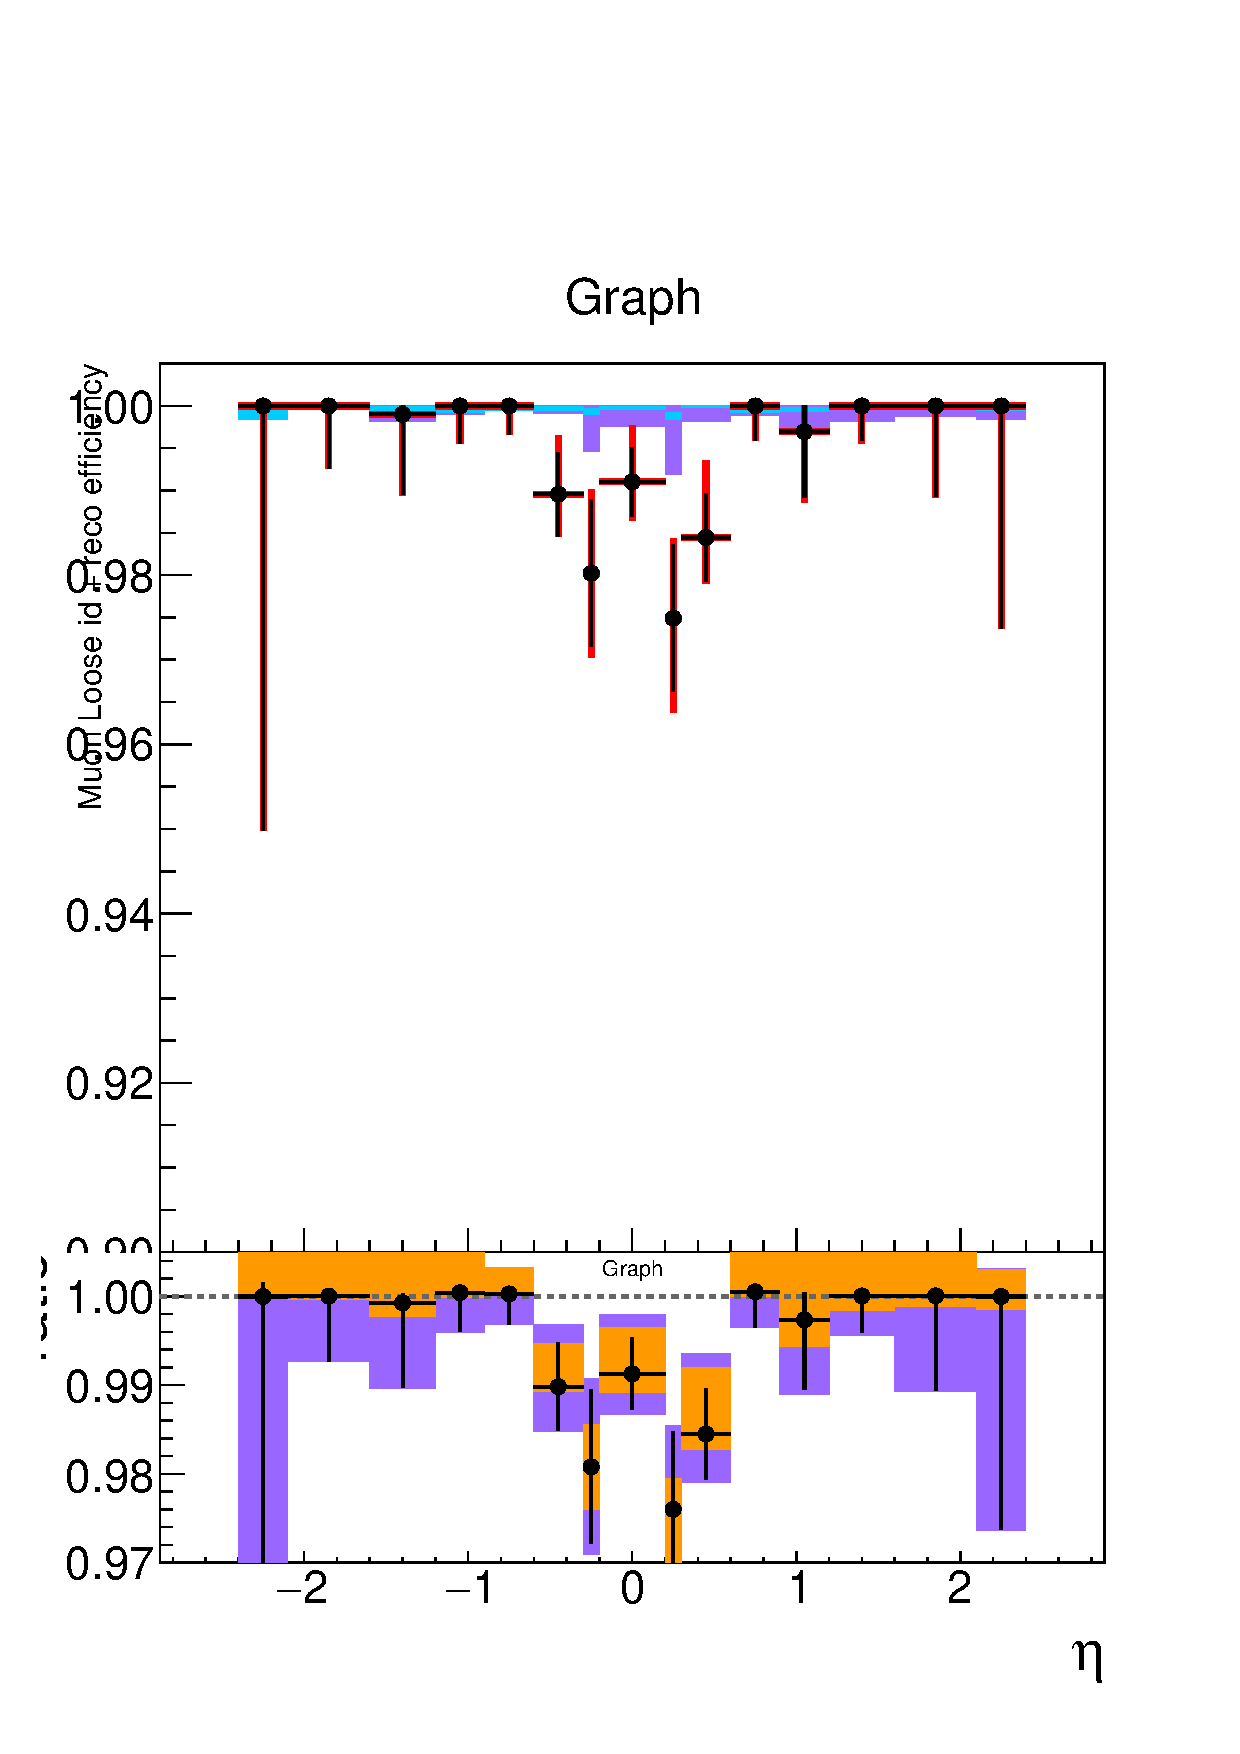
\includegraphics[width=2in]{Figures/Muons/mu_Loose_pt7.pdf}
\caption{}
\end{subfigure}
    \caption{Muon reconstruction and identification efficiency at low $\pt$, measured with the tag-and-probe method on $\JPsi$ events, as function of $\pt$ in the barrel (a) and end caps (b), and as function of $\eta$ for $\pt > 7\ \GeV$ (c). In the upper panel of each graph, the larger error bars include also the systematical uncertainties, while the smaller ones are purely statistical. Each graph's lower panel shows the ratio of the two efficiencies, the black error bars are for the statistical uncertainty, the orange rectangles for the systematic uncertainty, and the violet rectangles include both uncertainties.}
\label{fig:MuonIDEff_1}
\end{figure}

%\begin{figure}[htbp]
%  \begin{center}
%    \subfigure[]{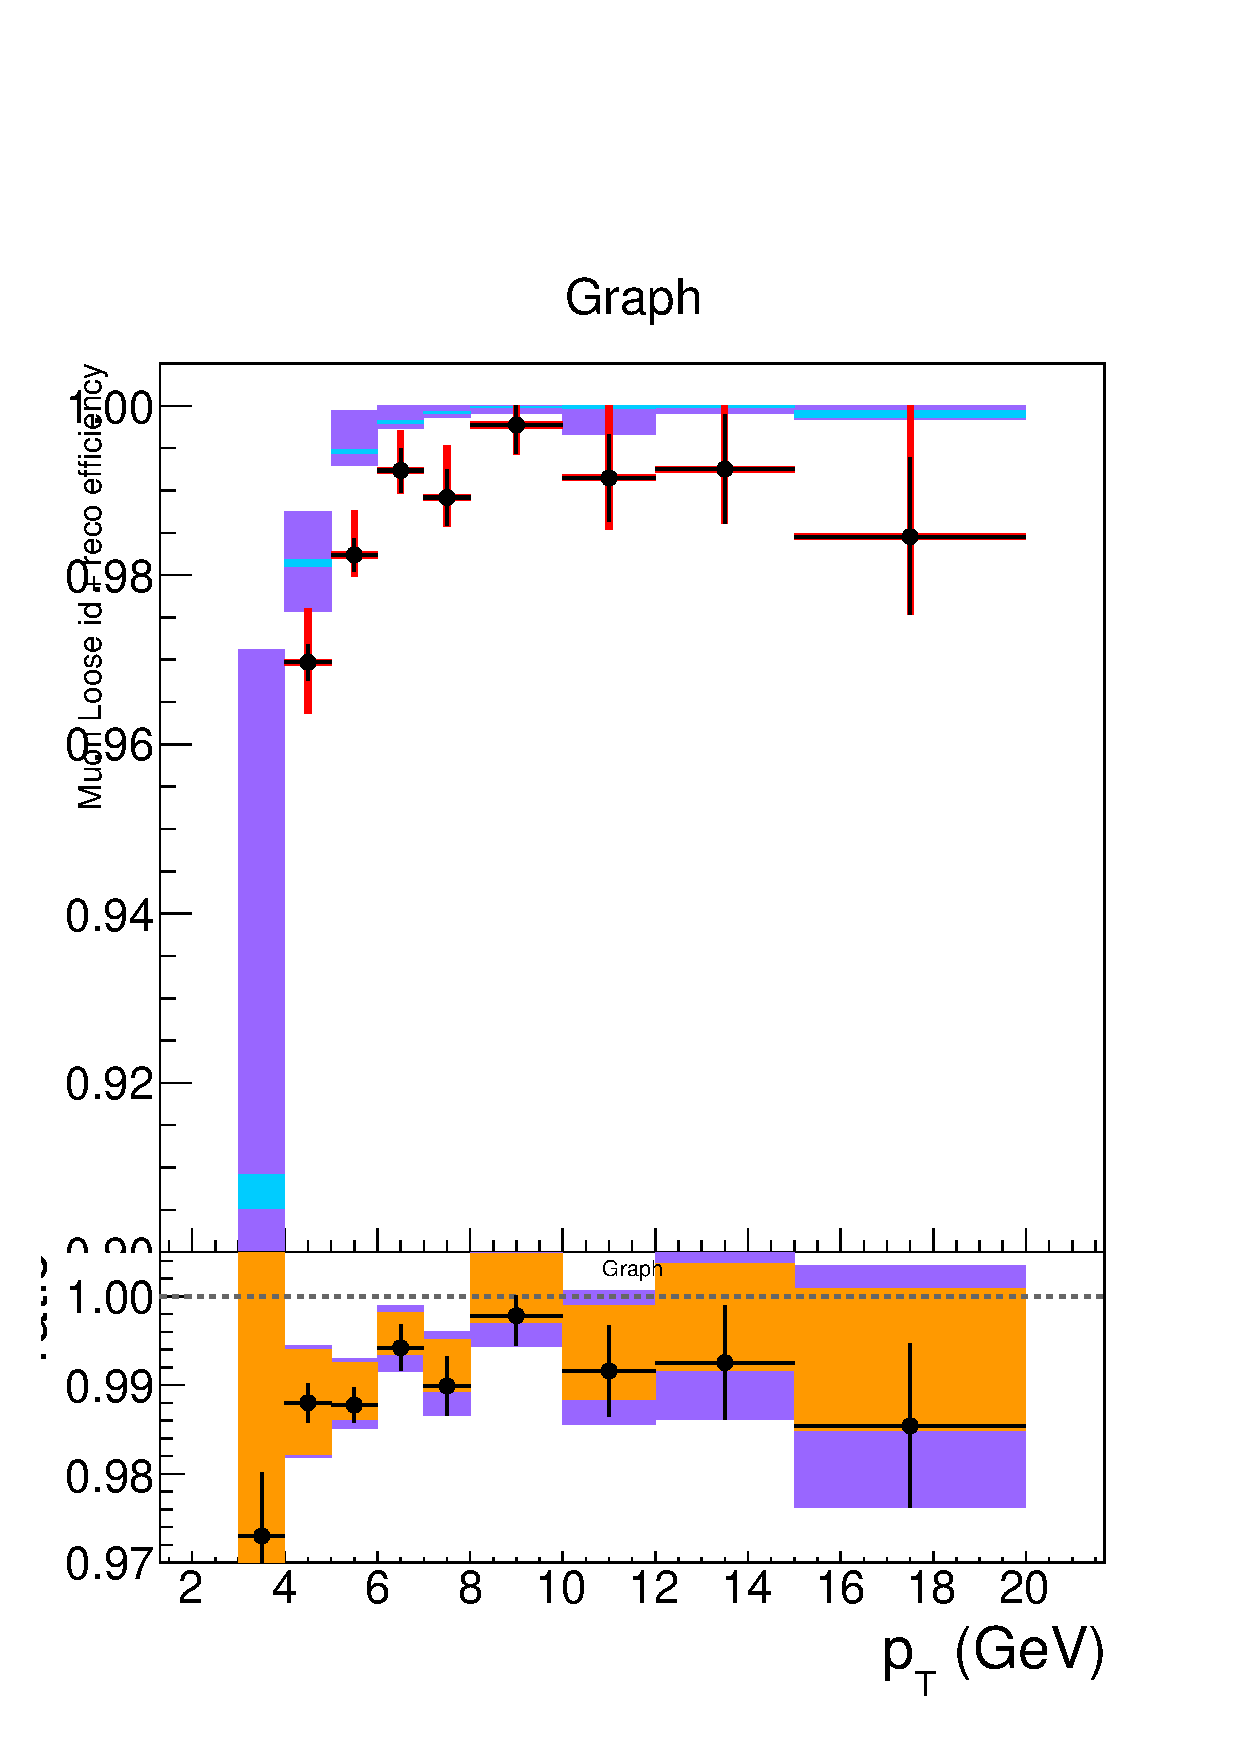
\includegraphics[width=0.32\textwidth]{Figures/Muons/mu_Loose_barrel.pdf}}
%    \subfigure[]{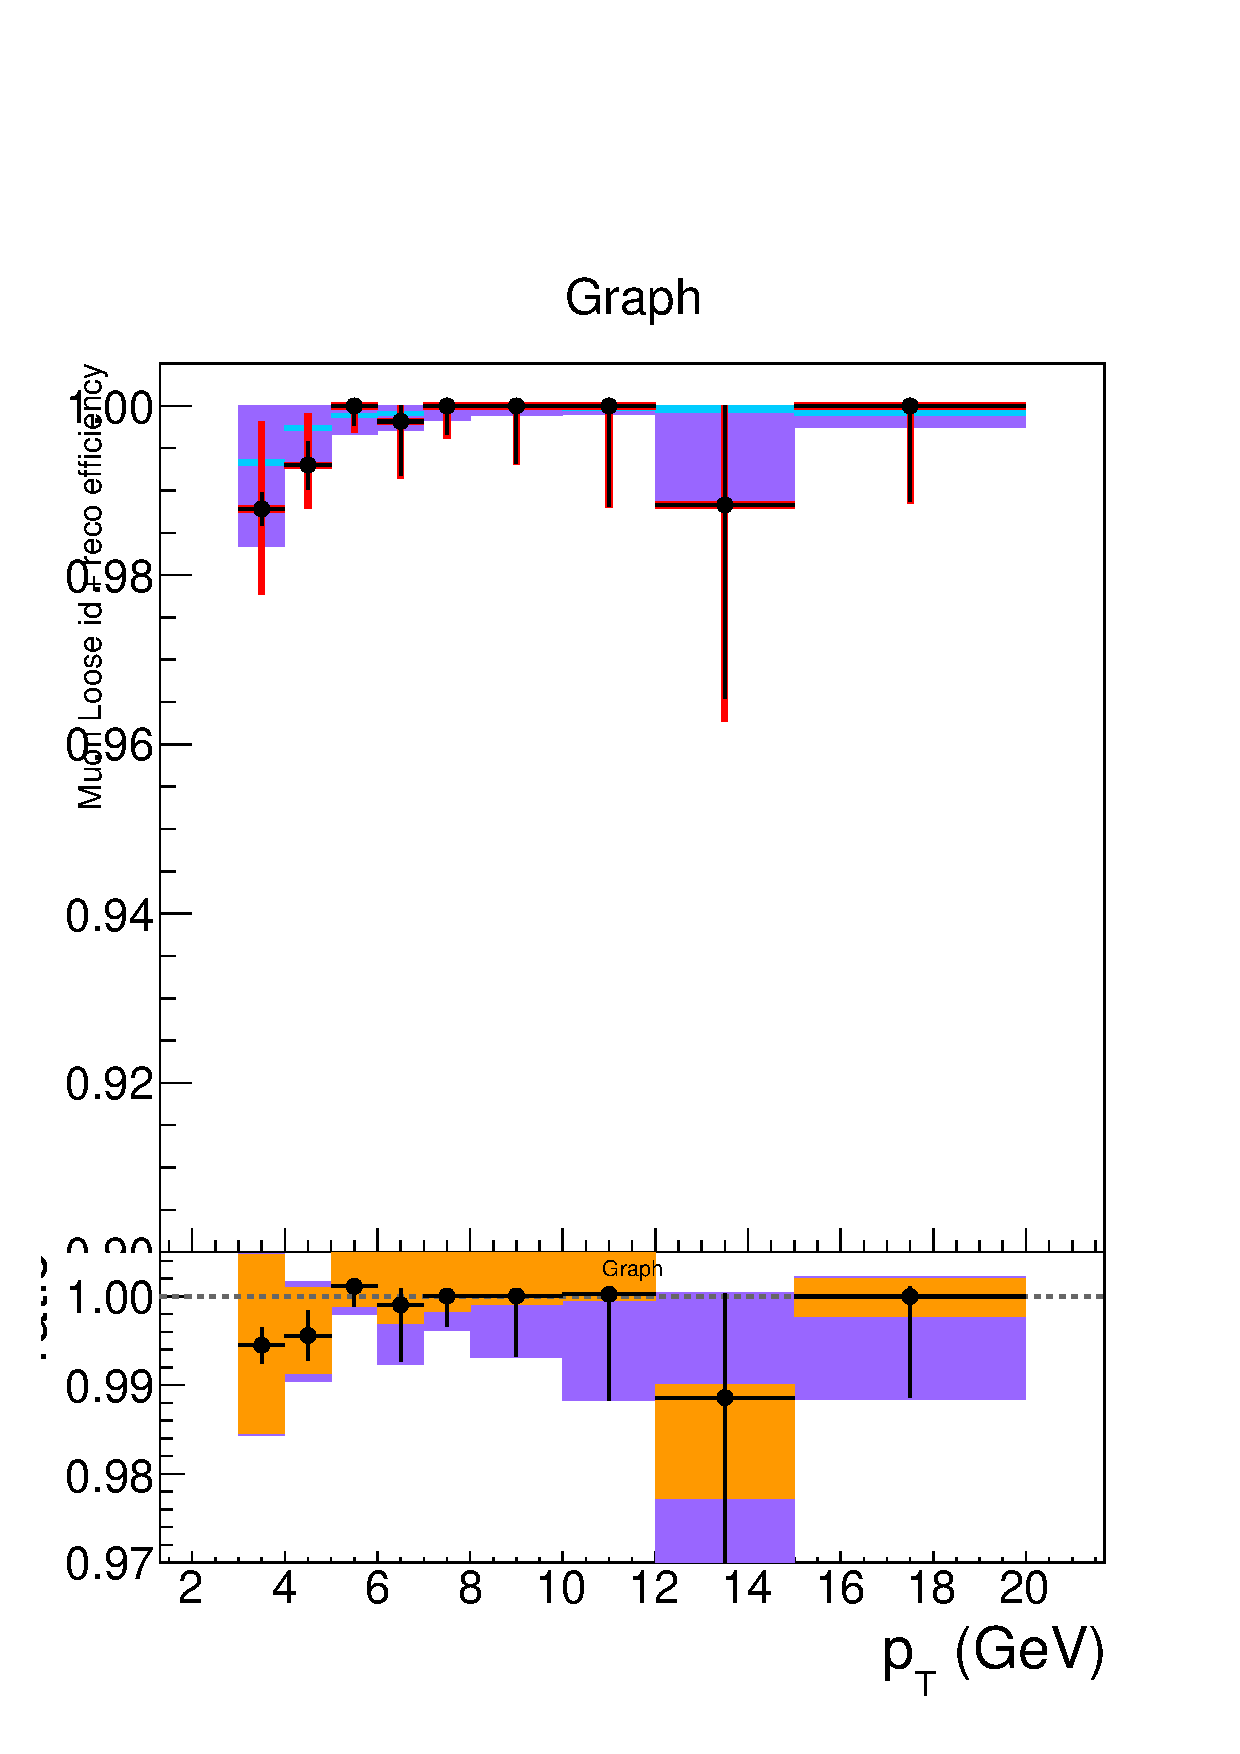
\includegraphics[width=0.32\textwidth]{Figures/Muons/mu_Loose_endcap.pdf}}
%    \subfigure[]{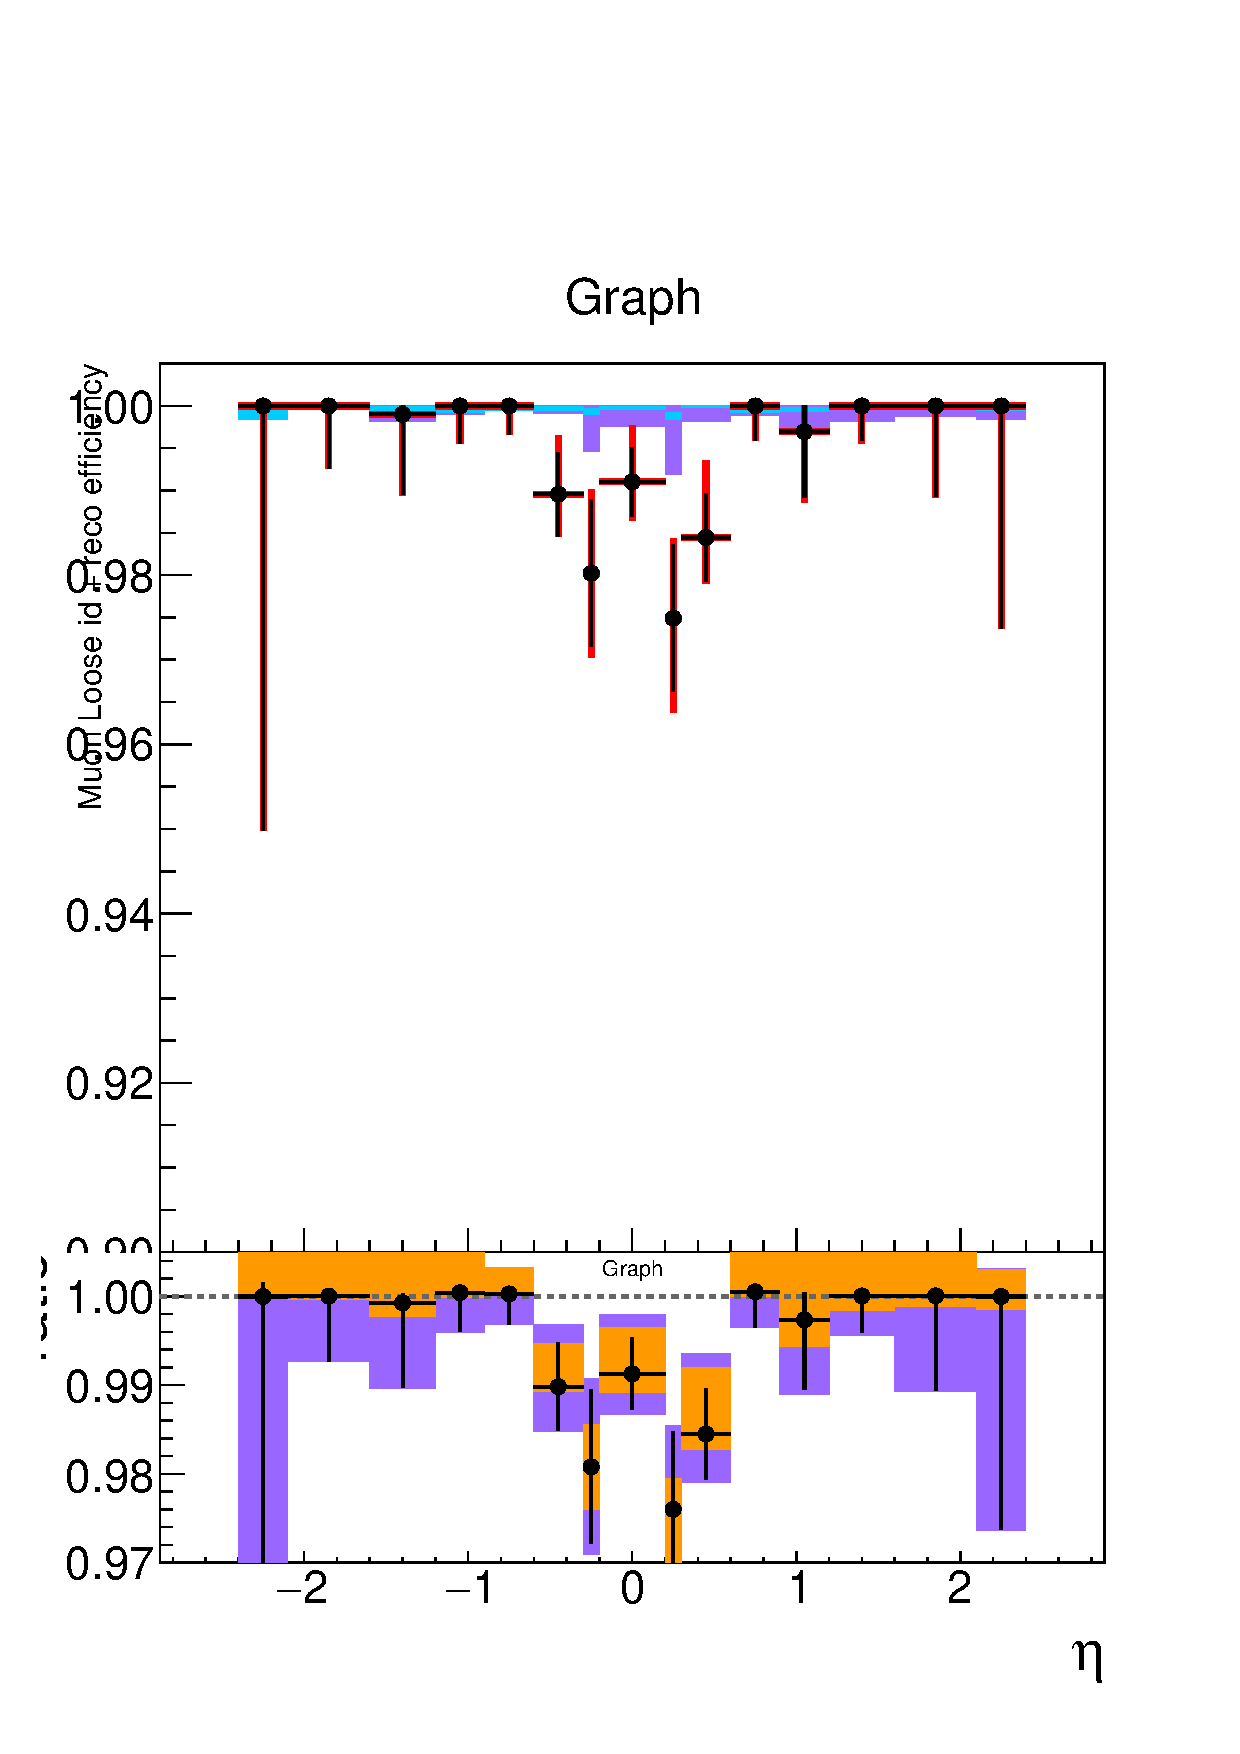
\includegraphics[width=0.32\textwidth]{Figures/Muons/mu_Loose_pt7.pdf}}
%    \caption{Muon reconstruction and identification efficiency at low \pt, measured with the tag\&probe method on \JPsi events, as function of \pt in the barrel (left) and endcaps (center), and as function of $\eta$ for $\pt > 7\GeV$ (right). In the upper panel, the larger error bars include also the systematical uncertainties, while the smaller ones are purely statistical. In the lower panel showing the ratio of the two efficiencies, the black error bars are for the statistical uncertainty, the orange rectangles for the systematical uncertainty and the violet rectangles include both uncertainties.}
%    \label{fig:MuonIDEff_1}
%\end{center}
%\end{figure}

\subsubsection{Impact parameter requirements}
The measurement is performed using $\Z$ events. Events are selected with HLT\_IsoMu20\_v* or HLT\_IsoMu22\_v* triggers.
For this measurement, the probe is a muon passing the POG Loose identification criteria,
and it is considered a passing probe if it satisfies the SIP3D, $d_{xy}$, $d_z$ cuts of this analysis.
The results are shown in Figure~\ref{fig:MuonIDEff_2}.
%Very good agreement between data and simulation is observed in the barrel (Fig.~\ref{fig:MuonIDEff_2}, left)
%while some inefficiency is visible in the endcaps, especially at large values of $|\eta|$.
%The data to simulation scale factor is found to be flat as function of \pt, so, similarly to what done
%for the identification part, we apply a correction only as function of $\eta$.


\begin{figure}[tbh]
\centering
\begin{subfigure}{0.3\textwidth}
\centering
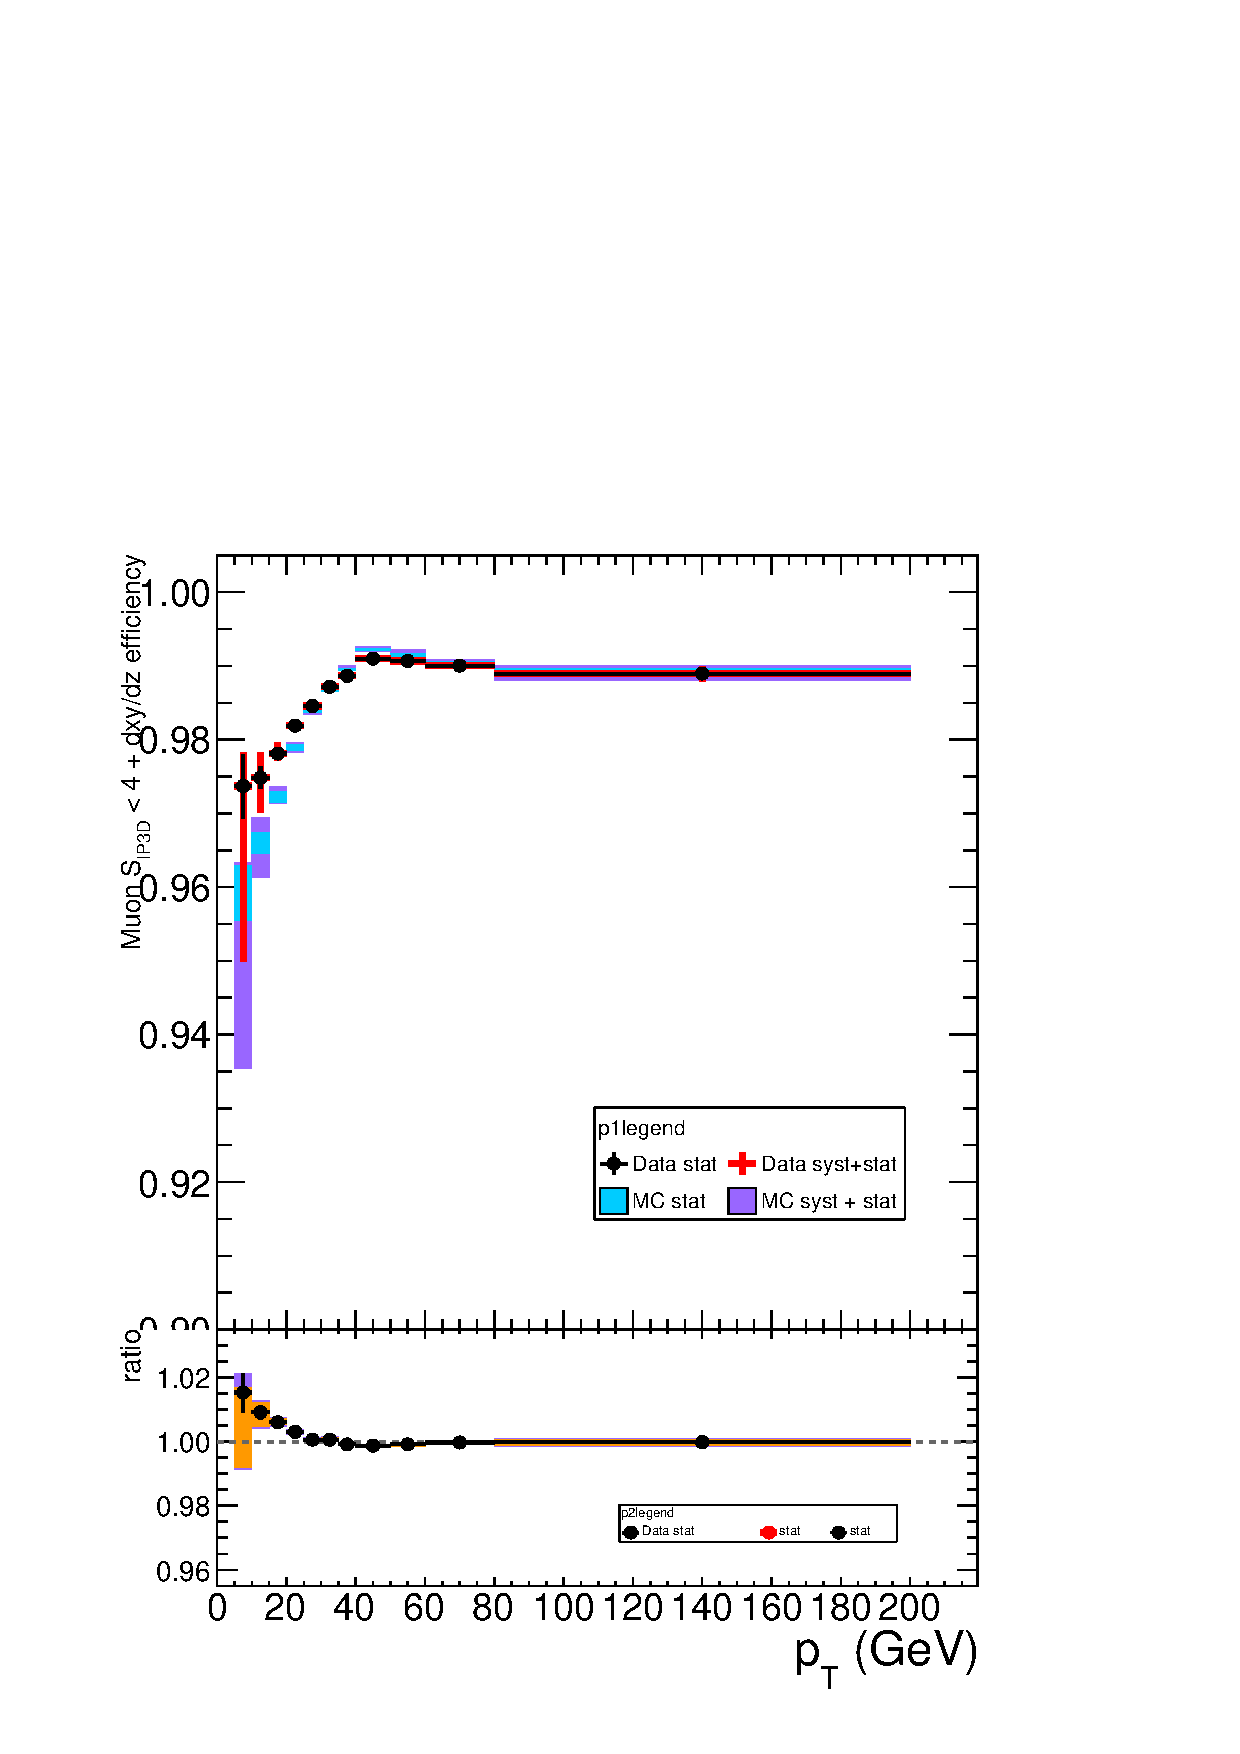
\includegraphics[width=2in]{Figures/Muons/mu_SIP4_barrel.pdf}
\caption{}
\end{subfigure}
\begin{subfigure}{0.3\textwidth}
\centering
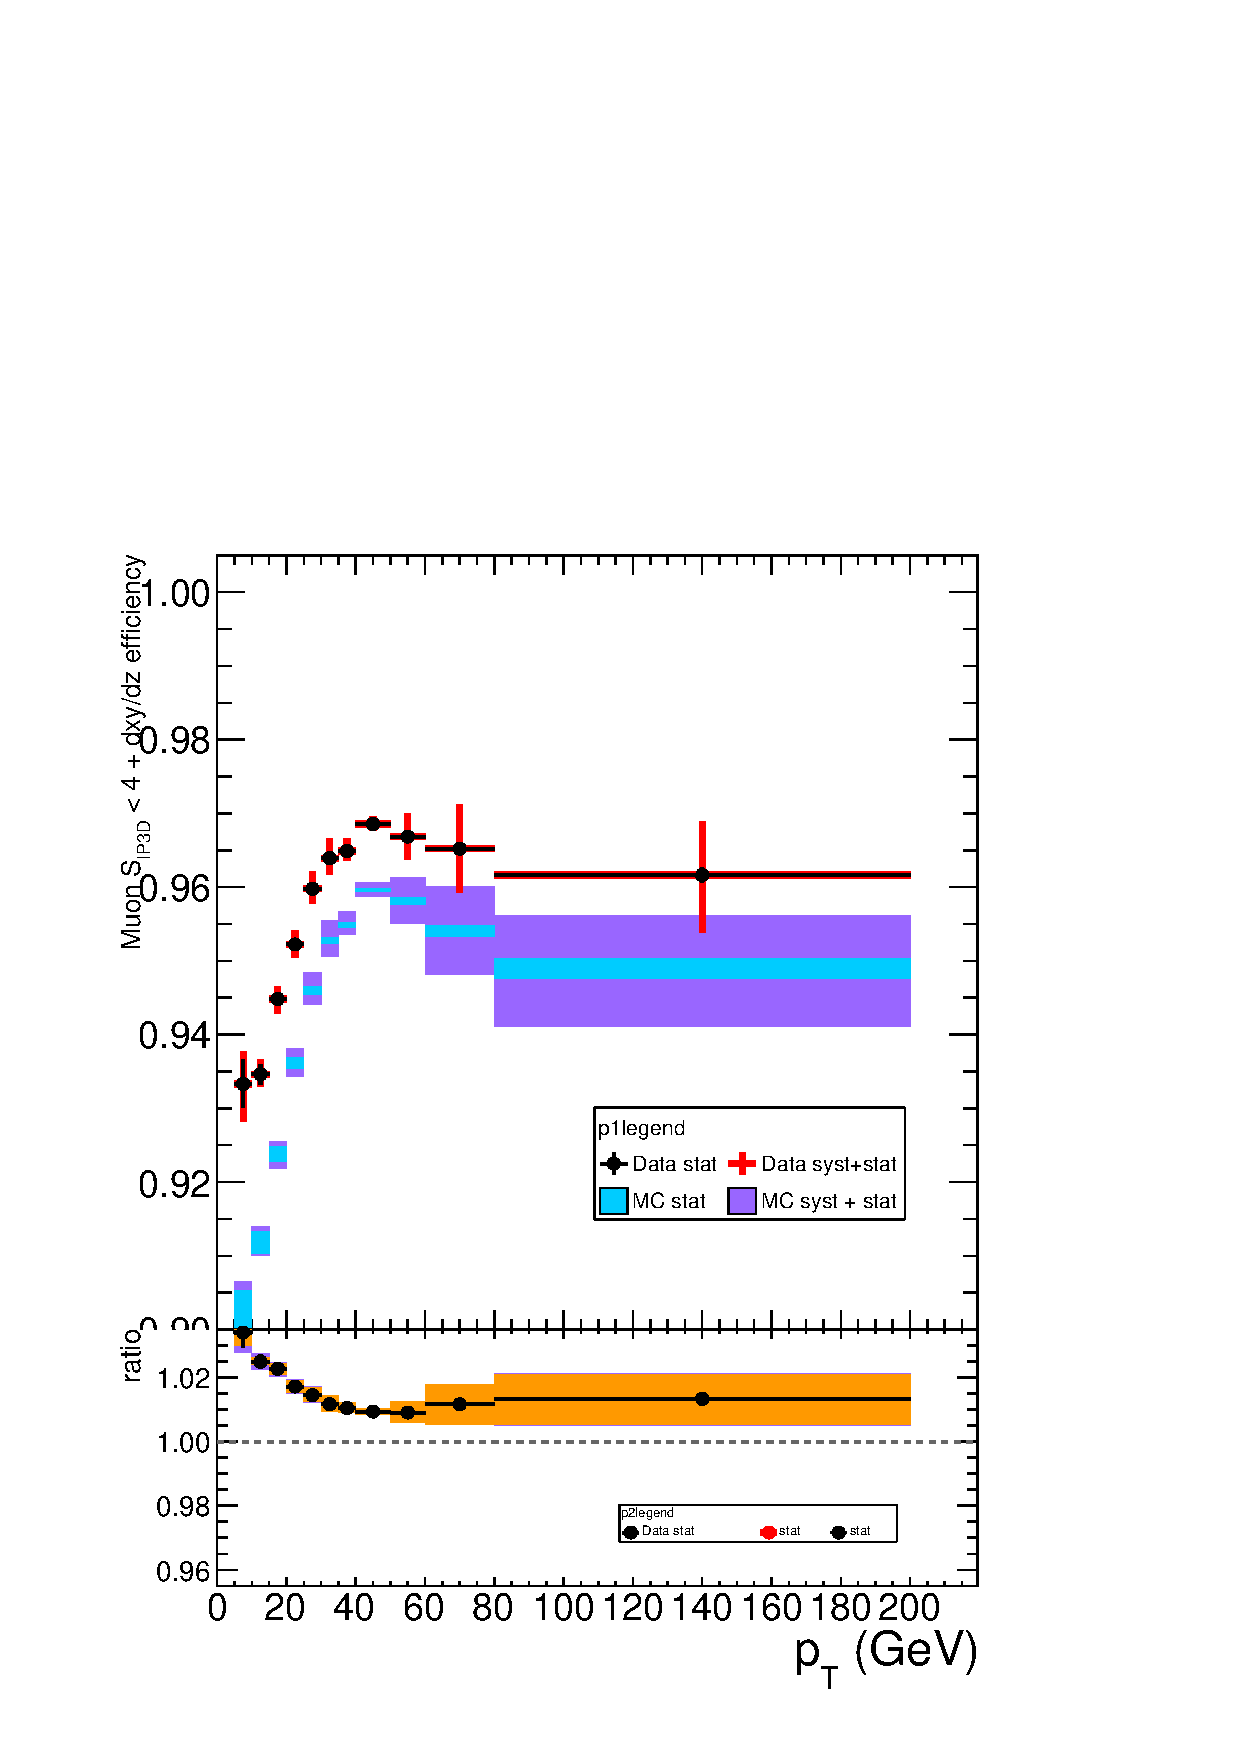
\includegraphics[width=2in]{Figures/Muons/mu_SIP4_endcap.pdf}
\caption{}
\end{subfigure}
\begin{subfigure}{0.3\textwidth}
\centering
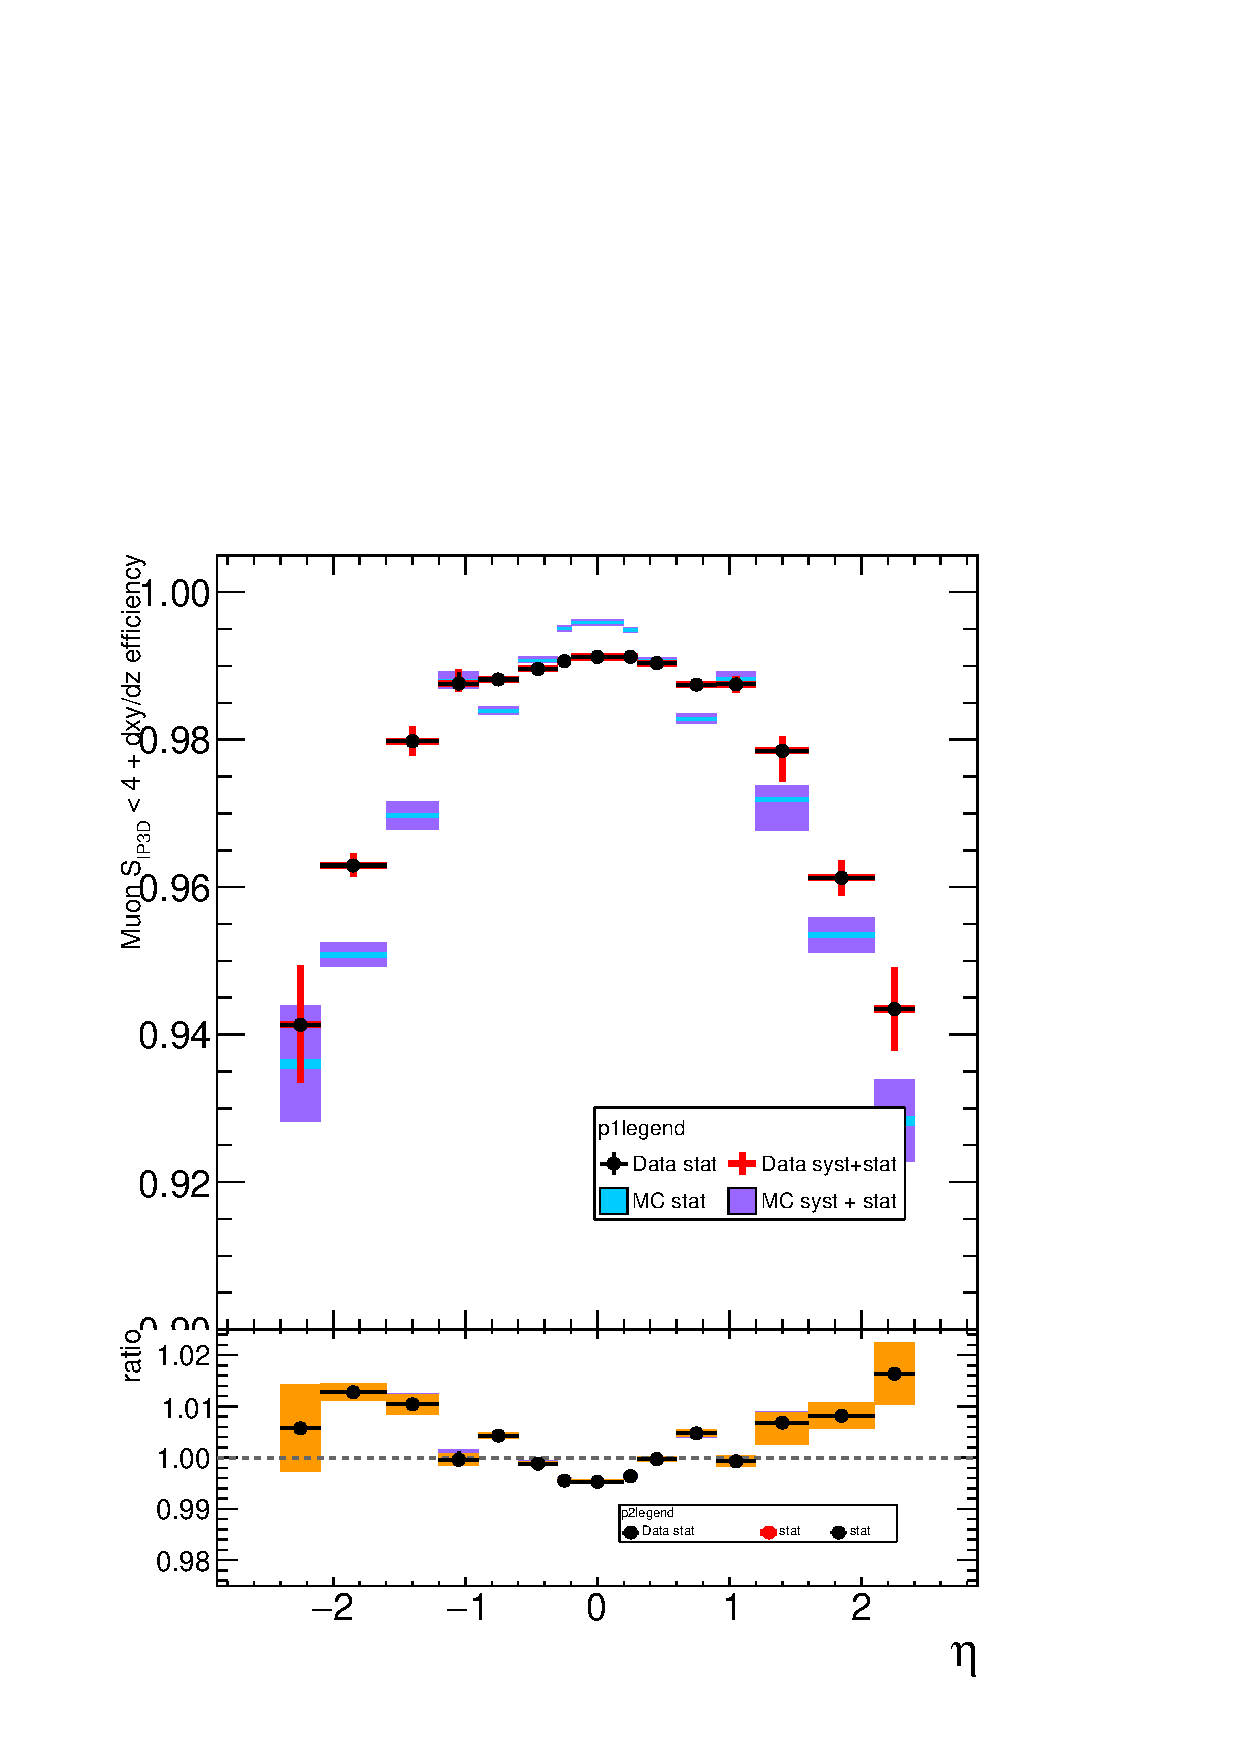
\includegraphics[width=2in]{Figures/Muons/mu_SIP4_pt20.pdf}
\caption{}
\end{subfigure}
\caption{Efficiency of the muon impact parameter requirements, measured with the tag-and-probe method on $Z$ events, as function of $\pt$ in the barrel (a) and end caps (b), and as function of $\eta$ for $\pt > 20\ \GeV$ (c). In the upper panel of each graph, the larger error bars include also the systematical uncertainties, while the smaller ones are purely statistical. Each graph's lower panel shows the ratio of the two efficiencies, the black error bars are for the statistical uncertainty, the orange rectangles for the systematical uncertainty, and the violet rectangles include both uncertainties.}
\label{fig:MuonIDEff_2}
\end{figure}

%\begin{figure}[htbp]
%  \begin{center}
%    \subfigure[]{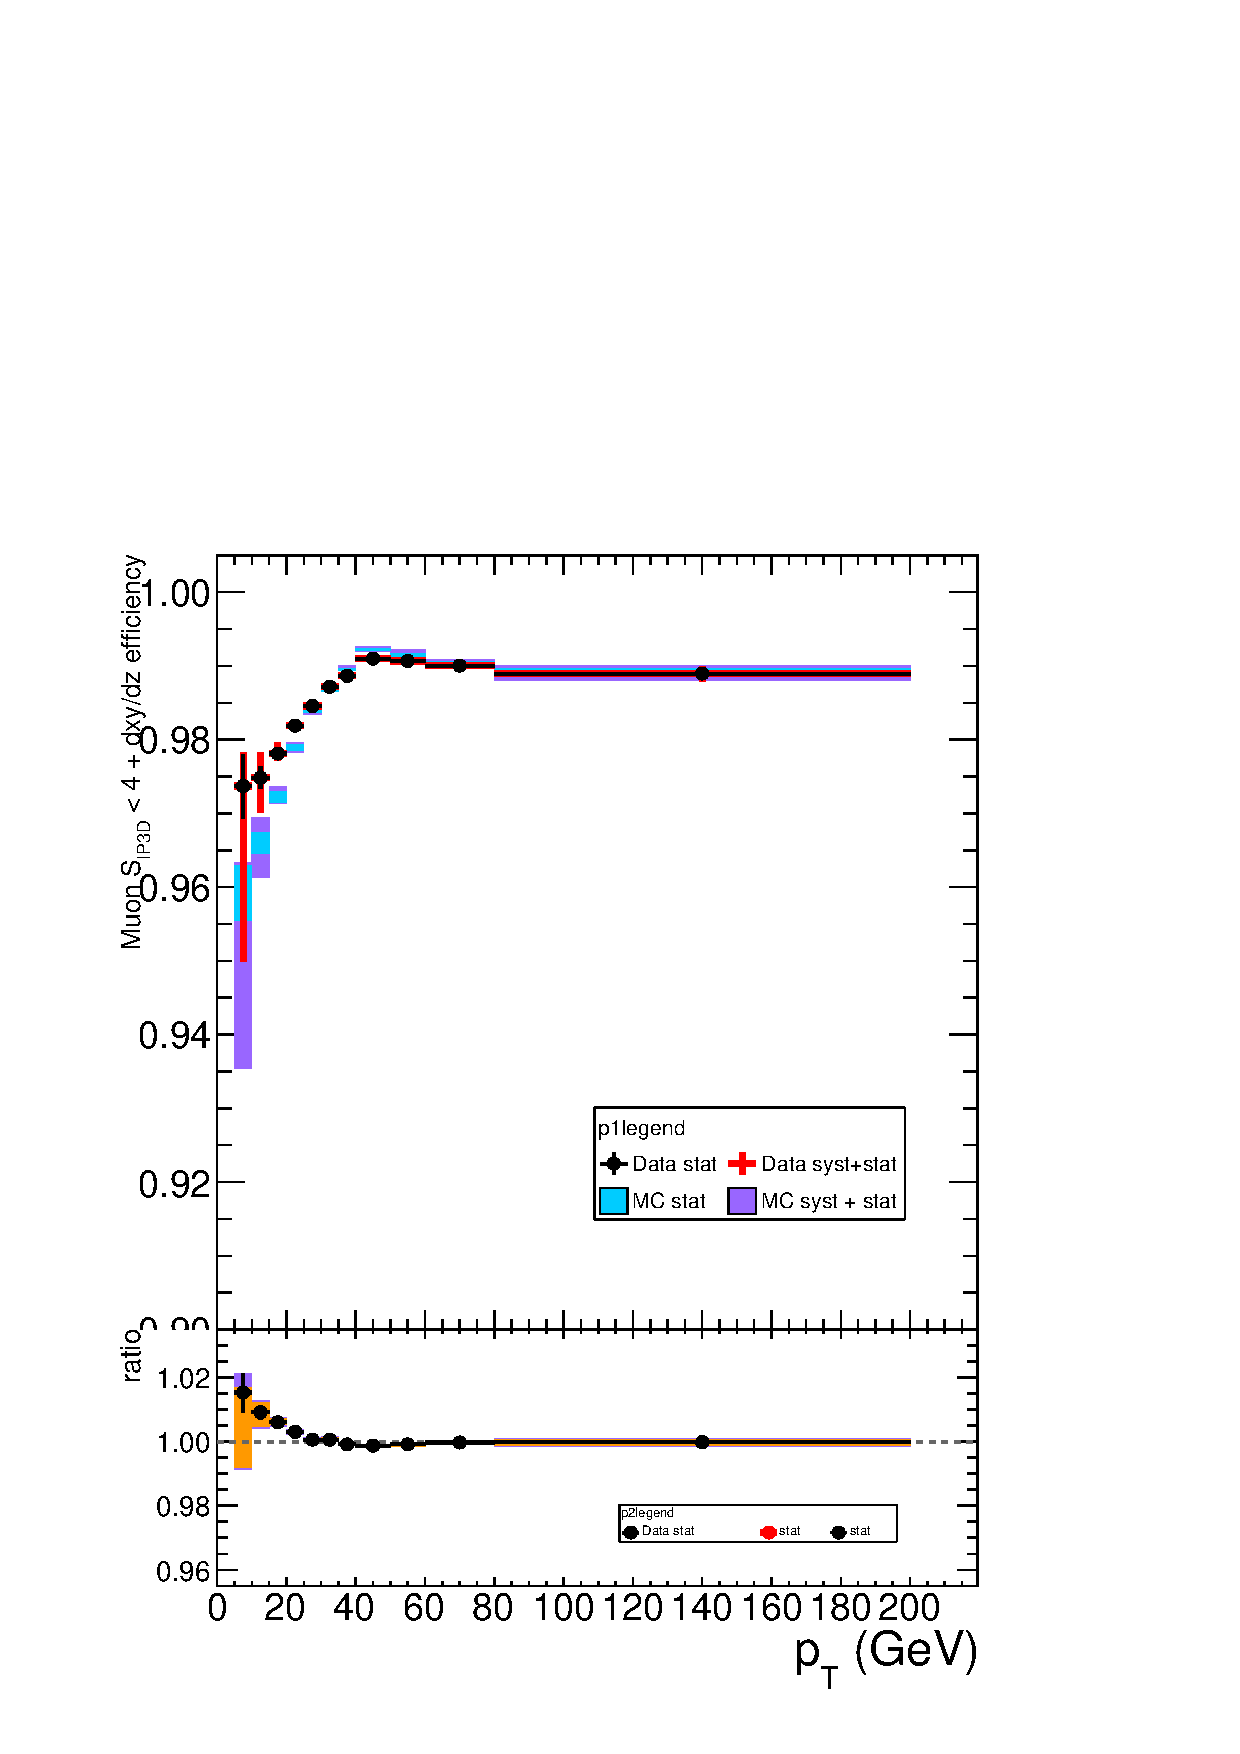
\includegraphics[width=0.32\textwidth]{Figures/Muons/mu_SIP4_barrel.pdf}}
%    \subfigure[]{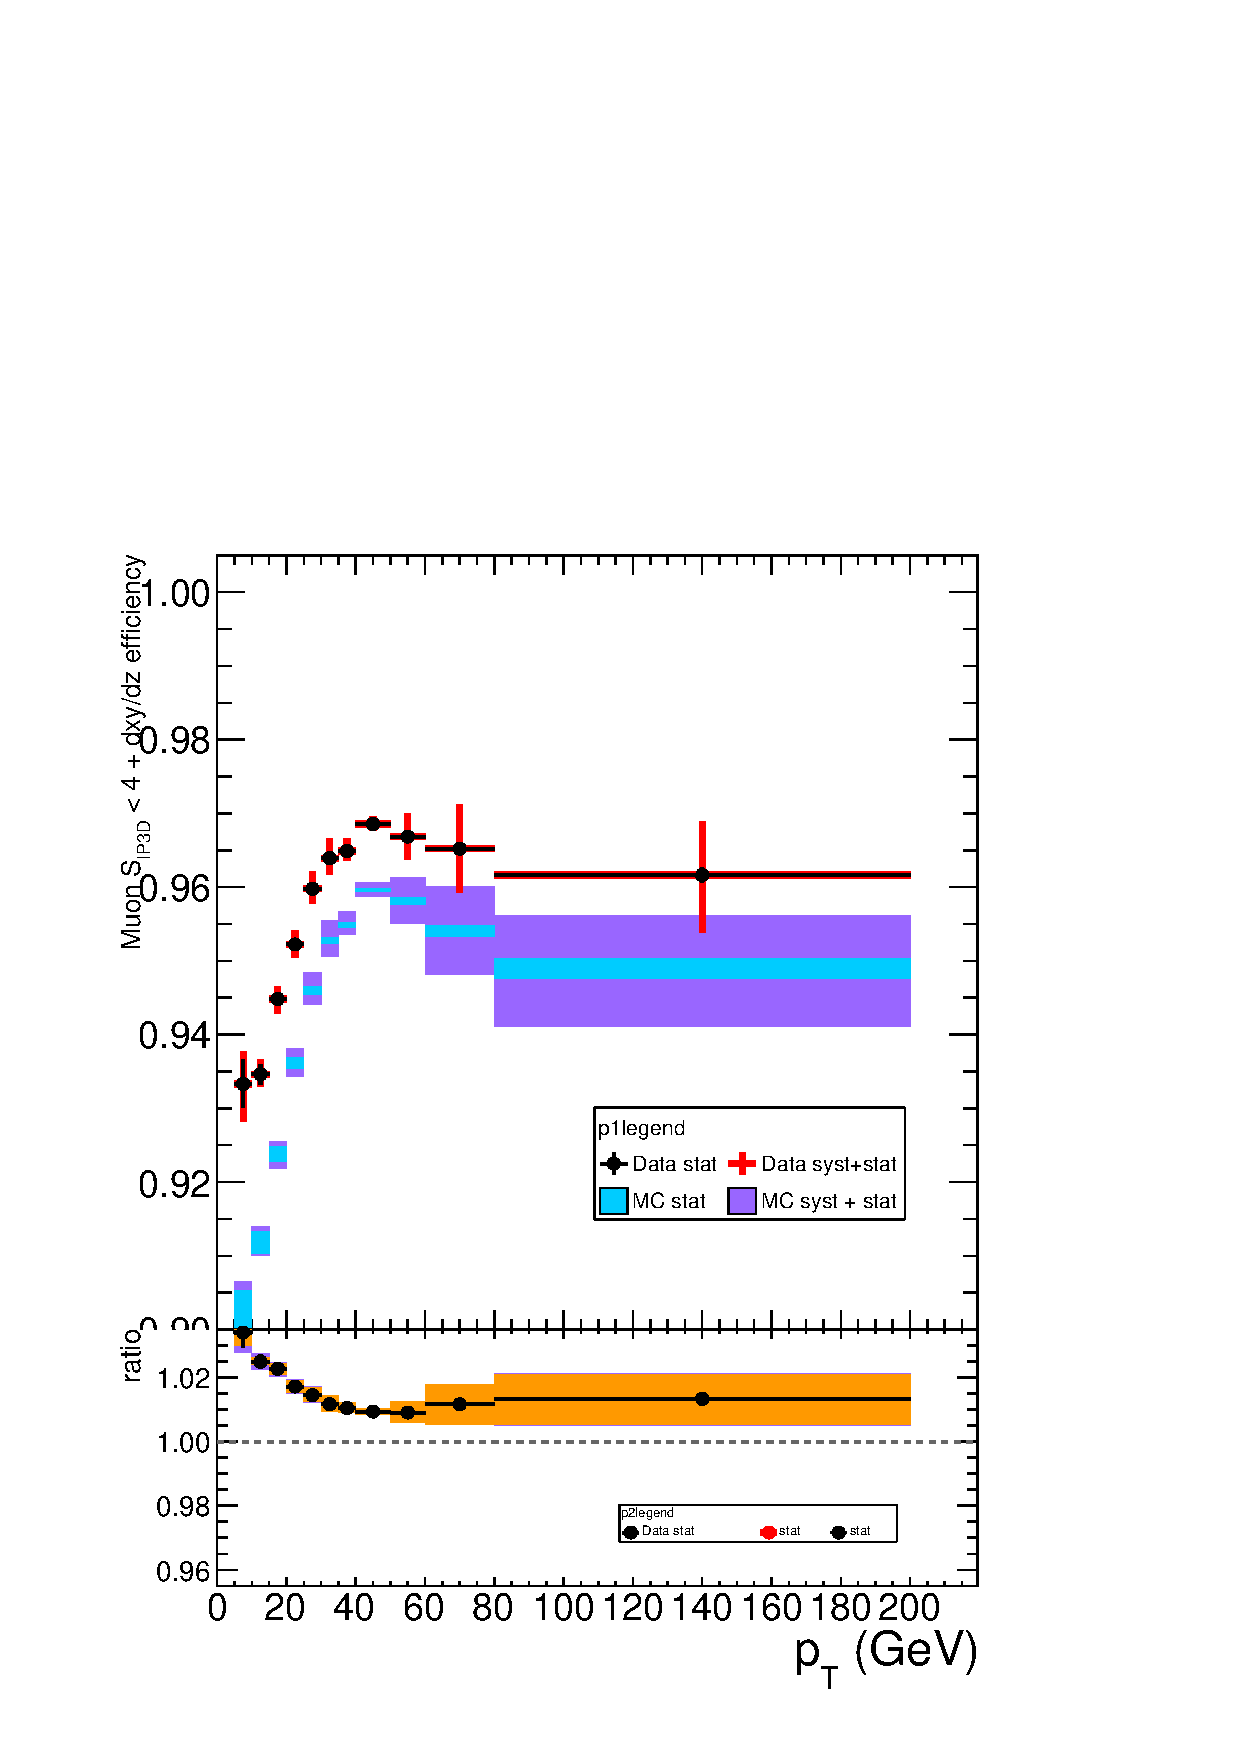
\includegraphics[width=0.32\textwidth]{Figures/Muons/mu_SIP4_endcap.pdf}}
%    \subfigure[]{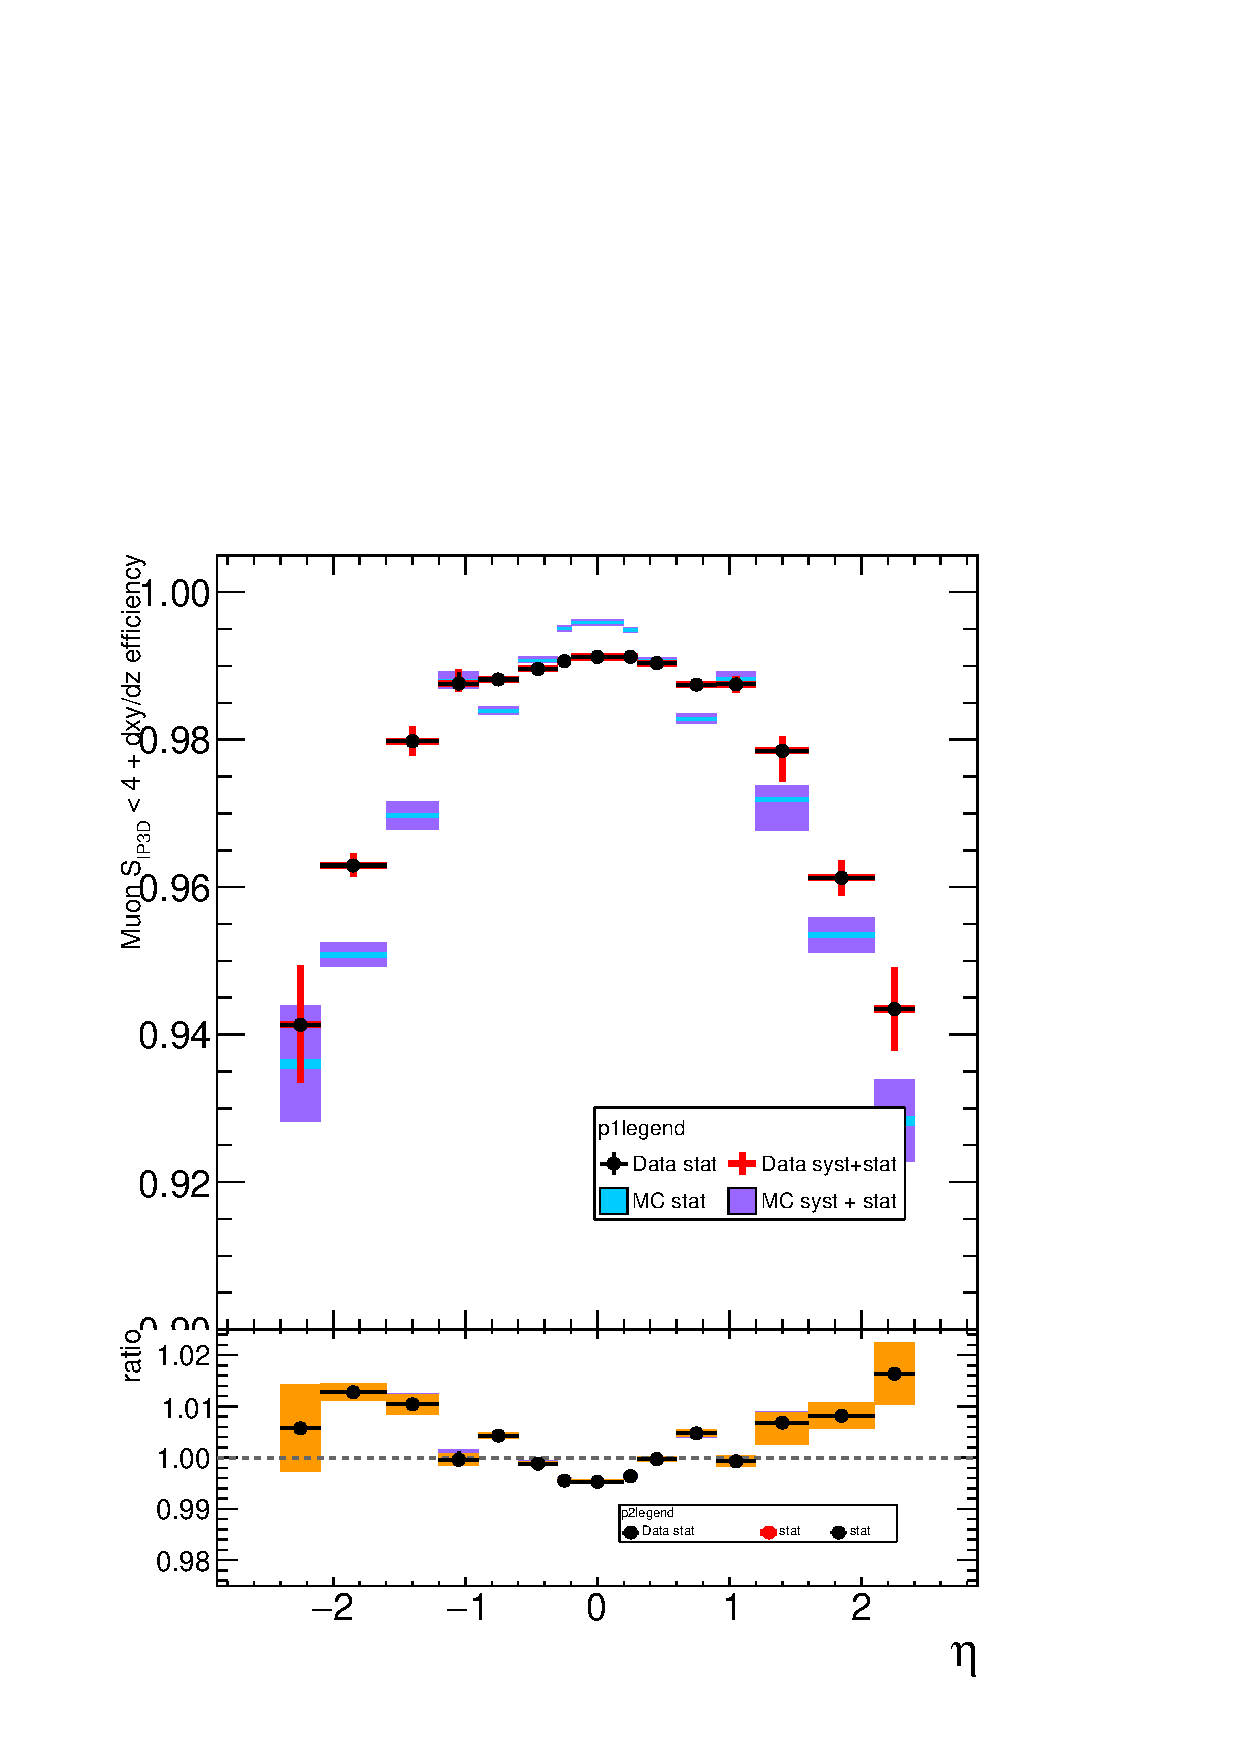
\includegraphics[width=0.32\textwidth]{Figures/Muons/mu_SIP4_pt20.pdf}}
%    \caption{Efficiency of the muon impact parameter requirements, measured with the tag\&probe method on \Z events, as function of \pt in the barrel (left) and endcaps (center), and as function of $\eta$ for $\pt > 20\GeV$ (right). In the upper panel, the larger error bars include also the systematical uncertainties, while the smaller ones are purely statistical. In the lower panel showing the ratio of the two efficiencies, the black error bars are for the statistical uncertainty, the orange rectangles for the systematical uncertainty and the violet rectangles include both uncertainties.}
%    \label{fig:MuonIDEff_2}
%\end{center}
%\end{figure}

\subsubsection{Isolation requirements}
The isolation efficiency is measured using events from the $\Z$ decay for any $\pt$, selected with either of HLT\_IsoMu20\_v* or HLT\_IsoMu22\_v* triggers. The isolation of the muons is calculated after recovery of the FSR photons and subtracting their contribution to the isolation cone of the muons \cite{AN-16-217}.
The results are shown in Figure~\ref{fig:MuonIDEff_3}.

\begin{figure}[tbh]
\centering
\begin{subfigure}{0.45\textwidth}
\centering
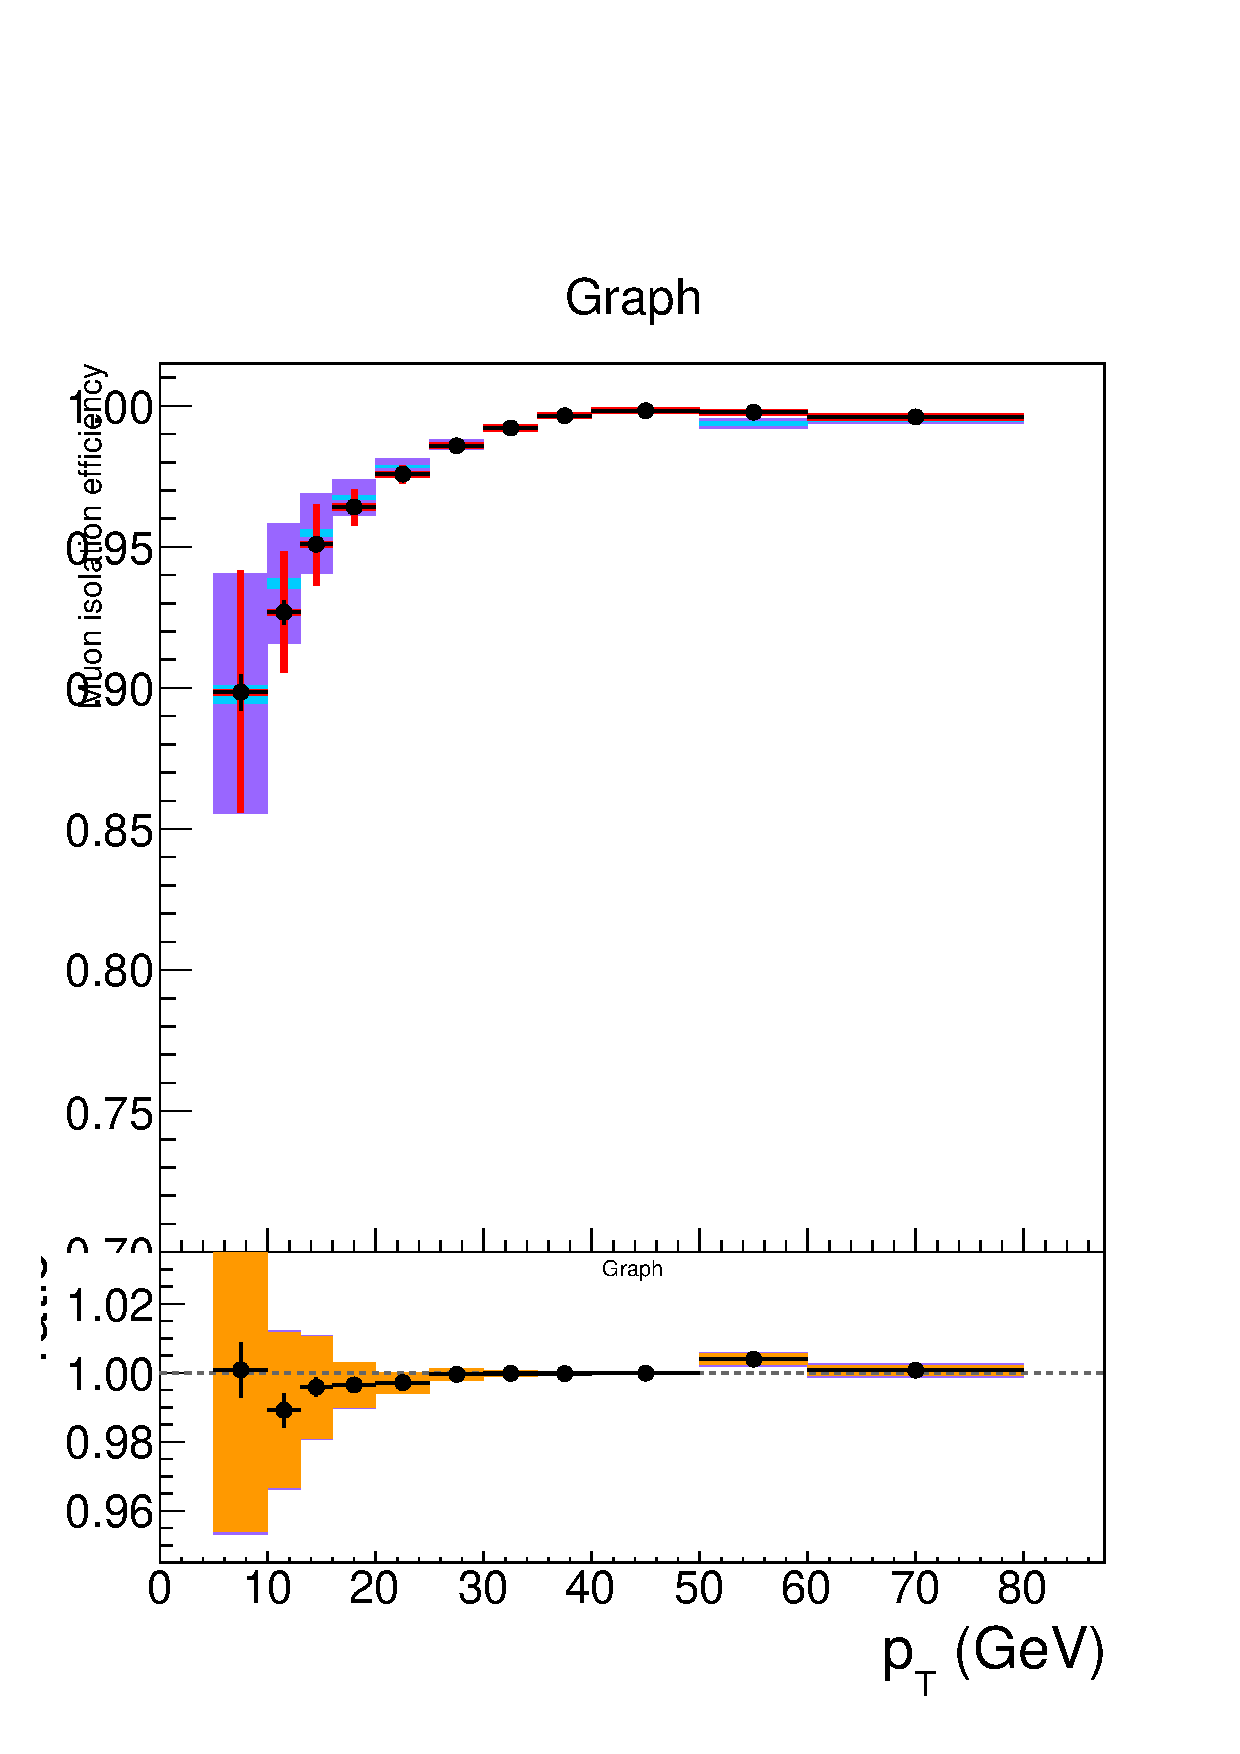
\includegraphics[width=3in]{Figures/Muons/mu_iso_barrel.pdf}
\caption{}
\end{subfigure}
\begin{subfigure}{0.45\textwidth}
\centering
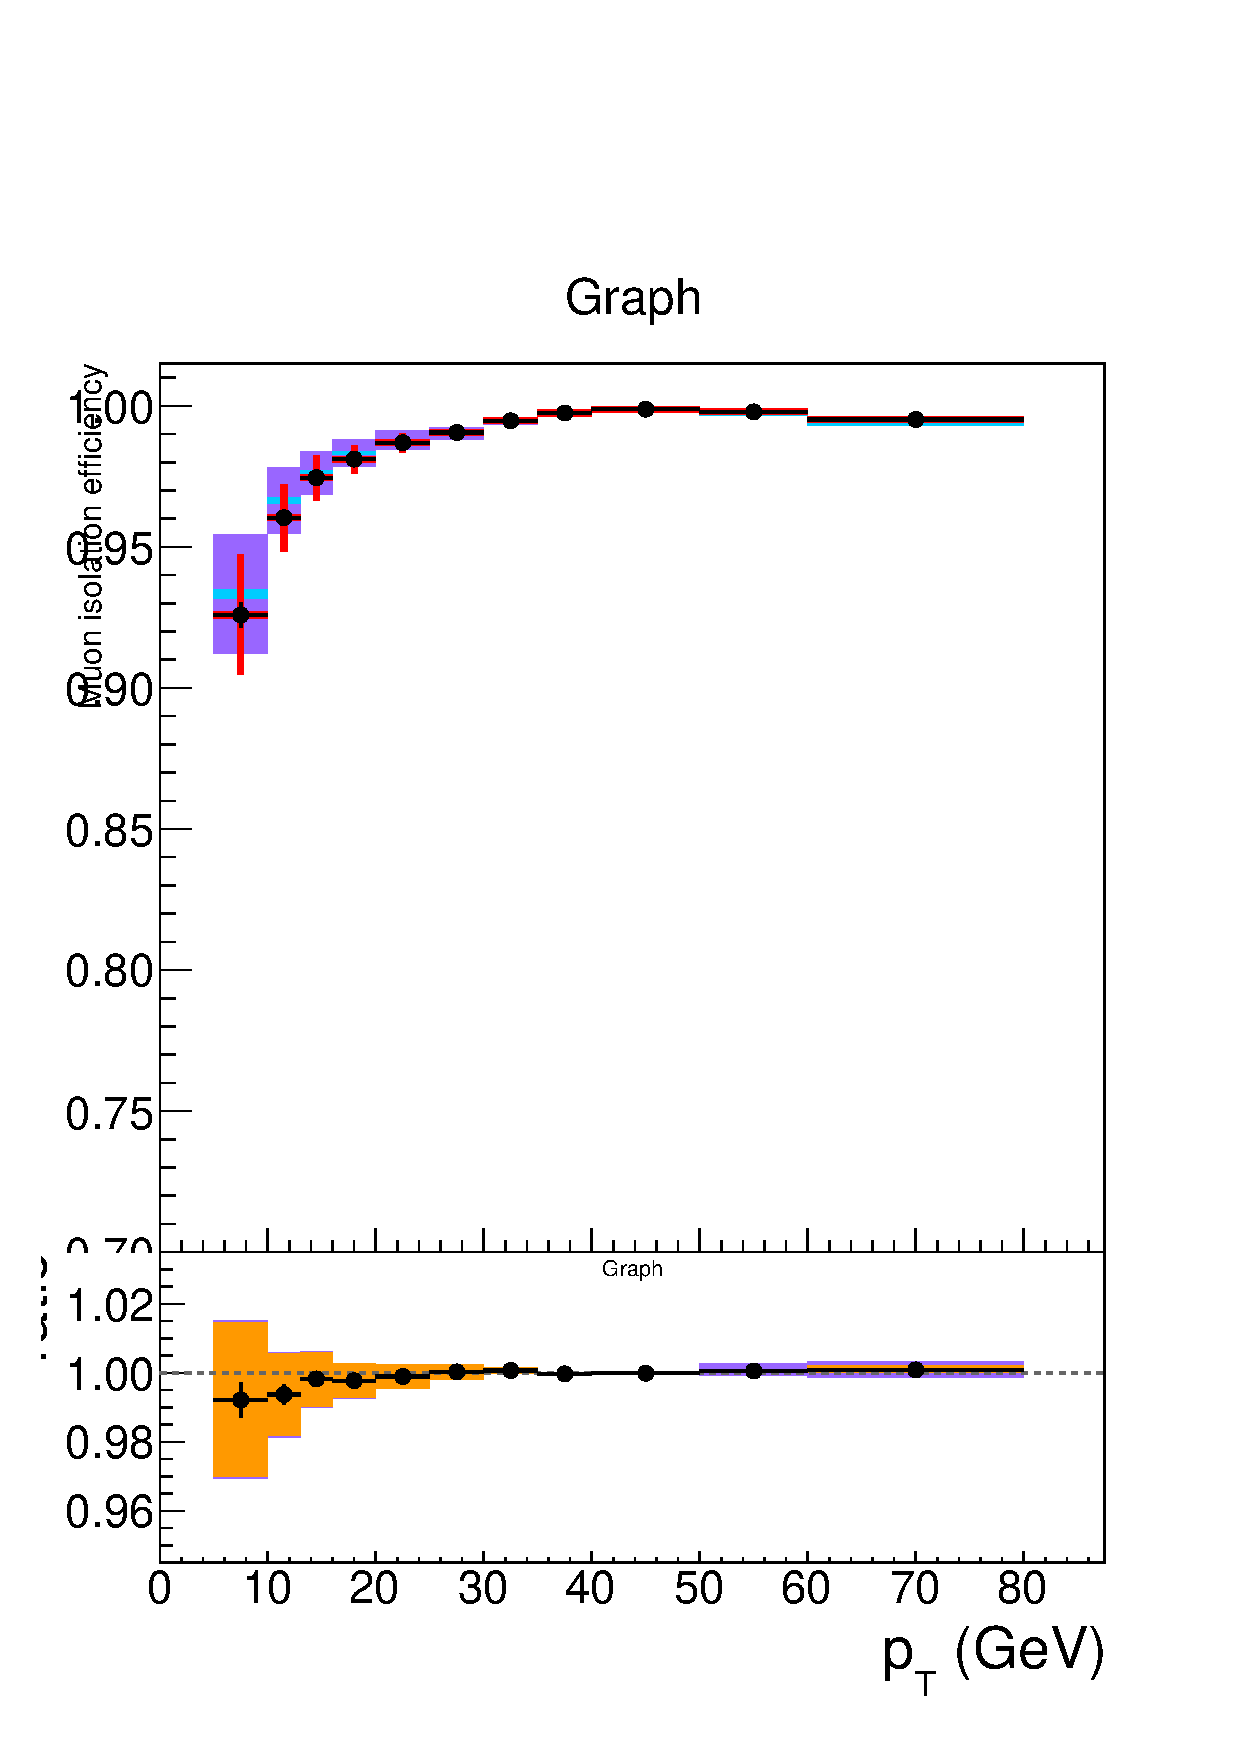
\includegraphics[width=3in]{Figures/Muons/mu_iso_endcap.pdf}
\caption{}
\end{subfigure}
    \caption{Efficiency of the muon isolation requirement, measured with the tag-and-probe method on $\Z$ events, as function of $\pt$ in the barrel (left) and end caps (right). In the upper panel of each graph, the larger error bars include also the systematical uncertainties, while the smaller ones are purely statistical. The lower panel of each graph shows the ratio of the two efficiencies, the black error bars are for the statistical uncertainty, the orange rectangles for the systematical uncertainty, and the violet rectangles include both uncertainties.}
\label{fig:MuonIDEff_3}
\end{figure}

%\begin{figure}[htbp]
%  \begin{center}
%    \subfigure[]{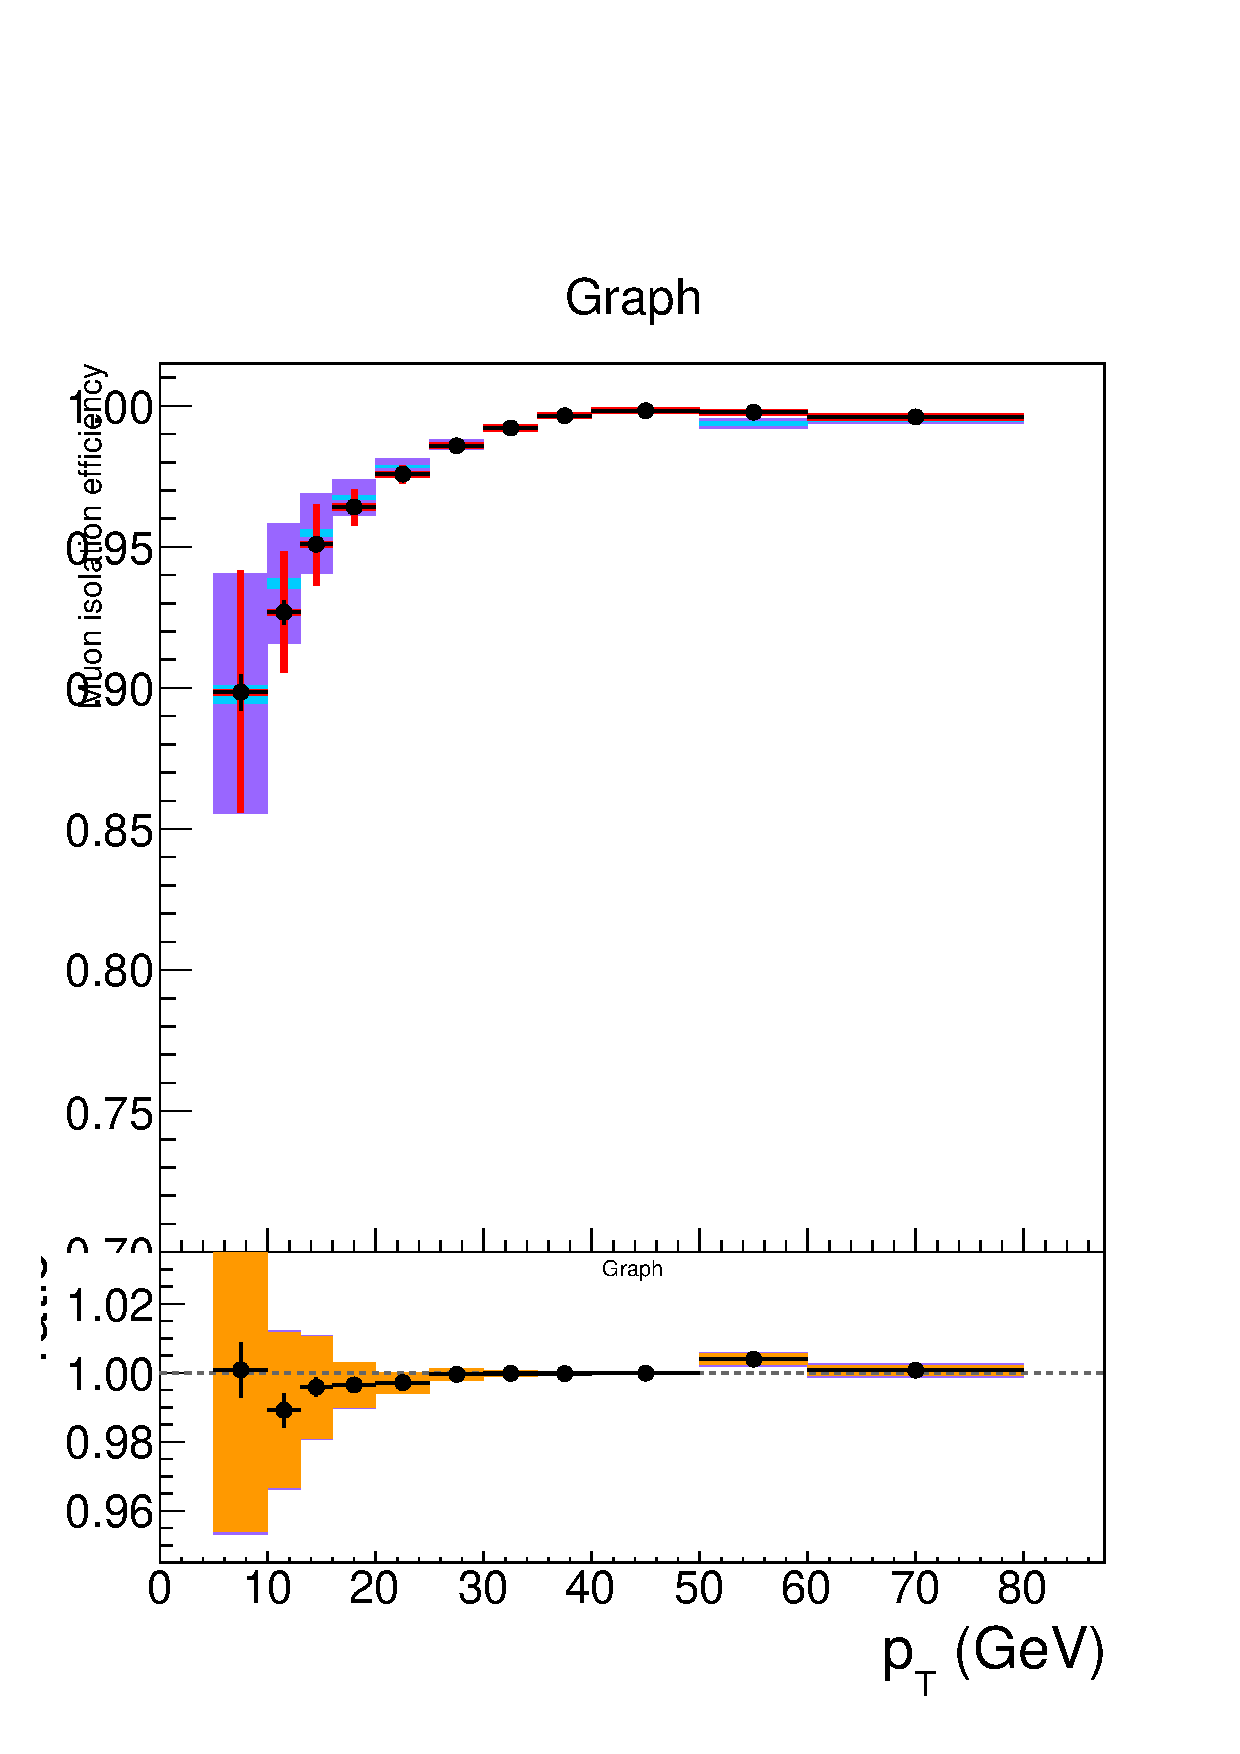
\includegraphics[width=0.32\textwidth]{Figures/Muons/mu_iso_barrel.pdf}}
%    \subfigure[]{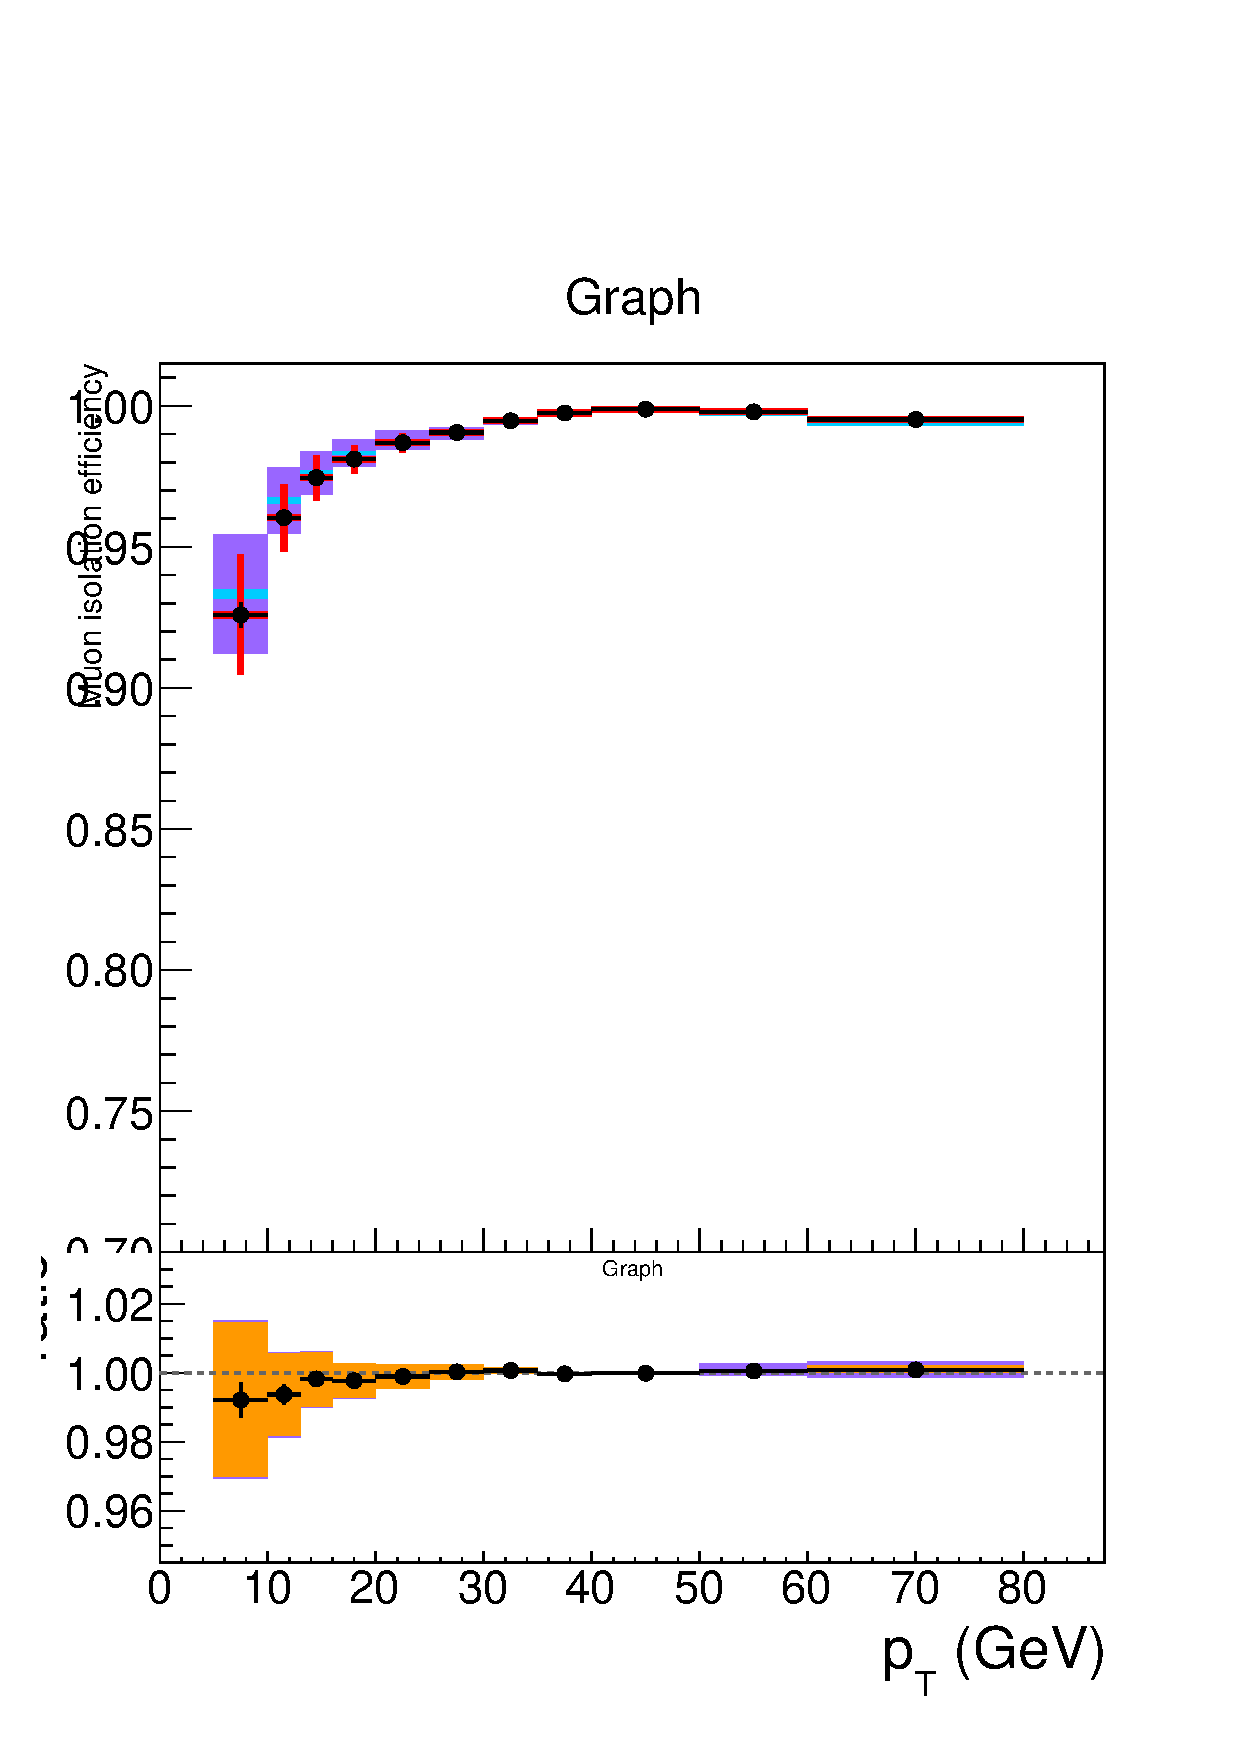
\includegraphics[width=0.32\textwidth]{Figures/Muons/mu_iso_endcap.pdf}}
%    \caption{Efficiency of the muon isolation requirement, measured with the tag\&probe method on \Z events, as function of \pt in the barrel (left) and endcaps (right). In the upper panel, the larger error bars include also the systematical uncertainties, while the smaller ones are purely statistical. In the lower panel showing the ratio of the two efficiencies, the black error bars are for the statistical uncertainty, the orange rectangles for the systematical uncertainty and the violet rectangles include both uncertainties.}
%    \label{fig:MuonIDEff_3}
%\end{center}
%\end{figure}

\subsubsection{Tracking}
The efficiency to reconstruct a muon track in the inner detector is measured using probes tracks
reconstructed in the muon system \cite{CMS_AN_2015-215}. The efficiency and 
data-to-MC scale factors are measured from $Z$ events as a function of $\eta$ for $\pt > 10\ \GeV$ and $\pt < 10\ \GeV$. The values of data-to-MC scale factors 
used are from the ReReco version of the full dataset collected in 2016. 
The tracking efficiency in data and simulation as a function of $\eta$ is shown in Figure~\ref{fig:MuonIDEff_4}.

\begin{figure}[tbh]
\centering
\begin{subfigure}{0.45\textwidth}
\centering
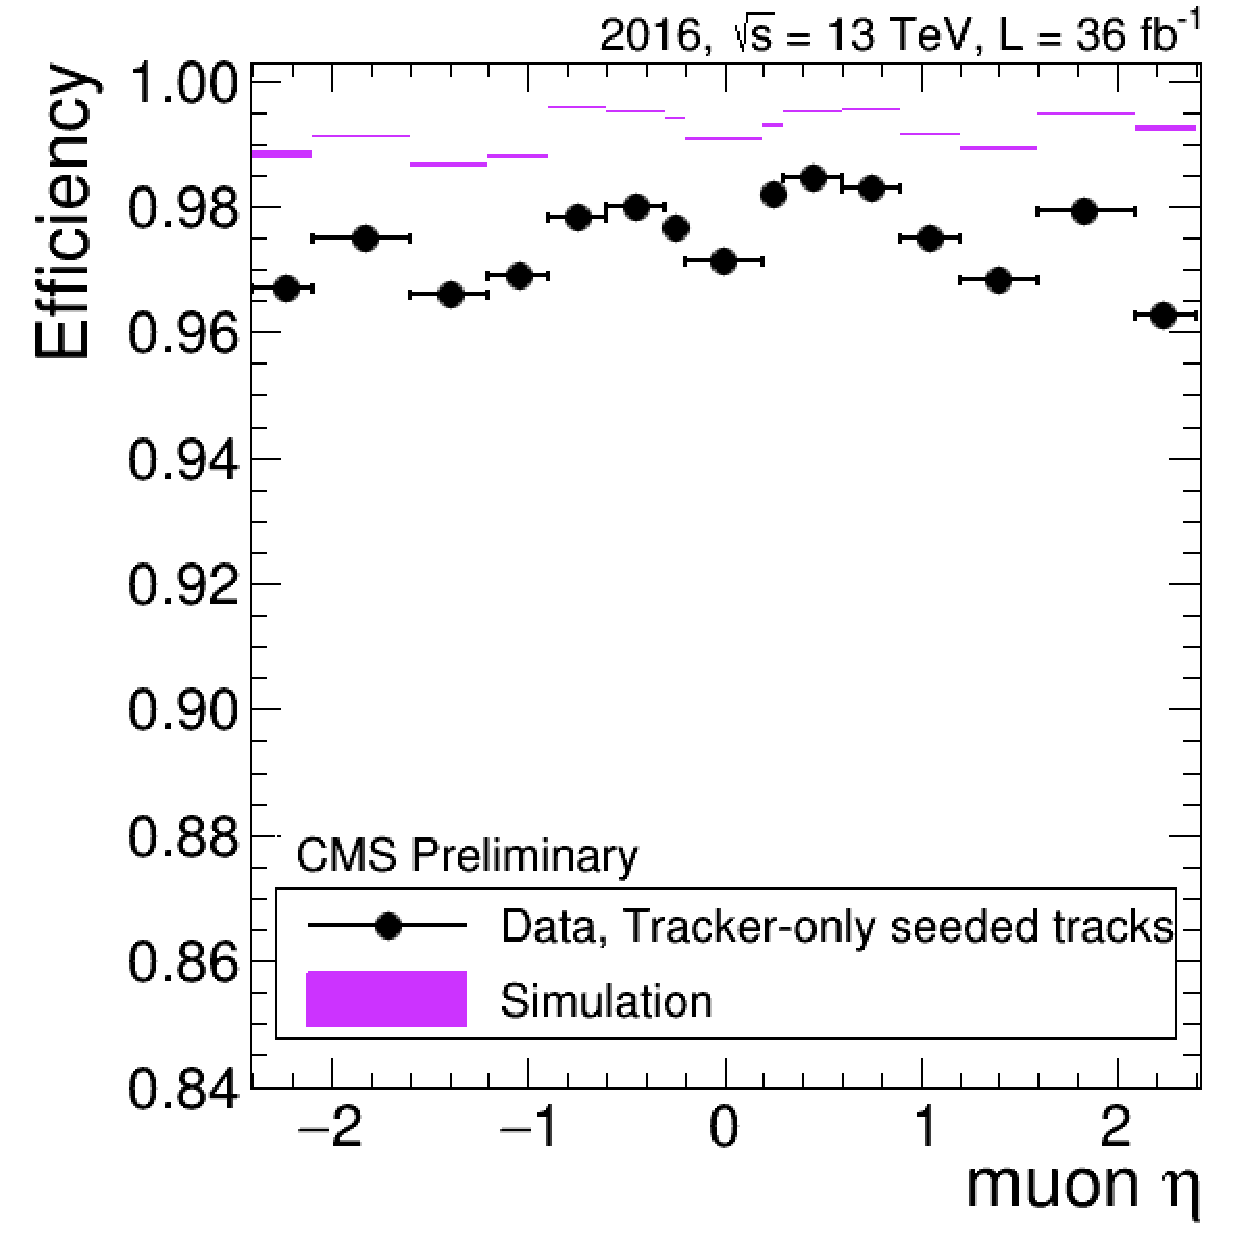
\includegraphics[width=3in]{Figures/Muons/trackingEffptl10.pdf}
\caption{}
\end{subfigure}
\begin{subfigure}{0.45\textwidth}
\centering
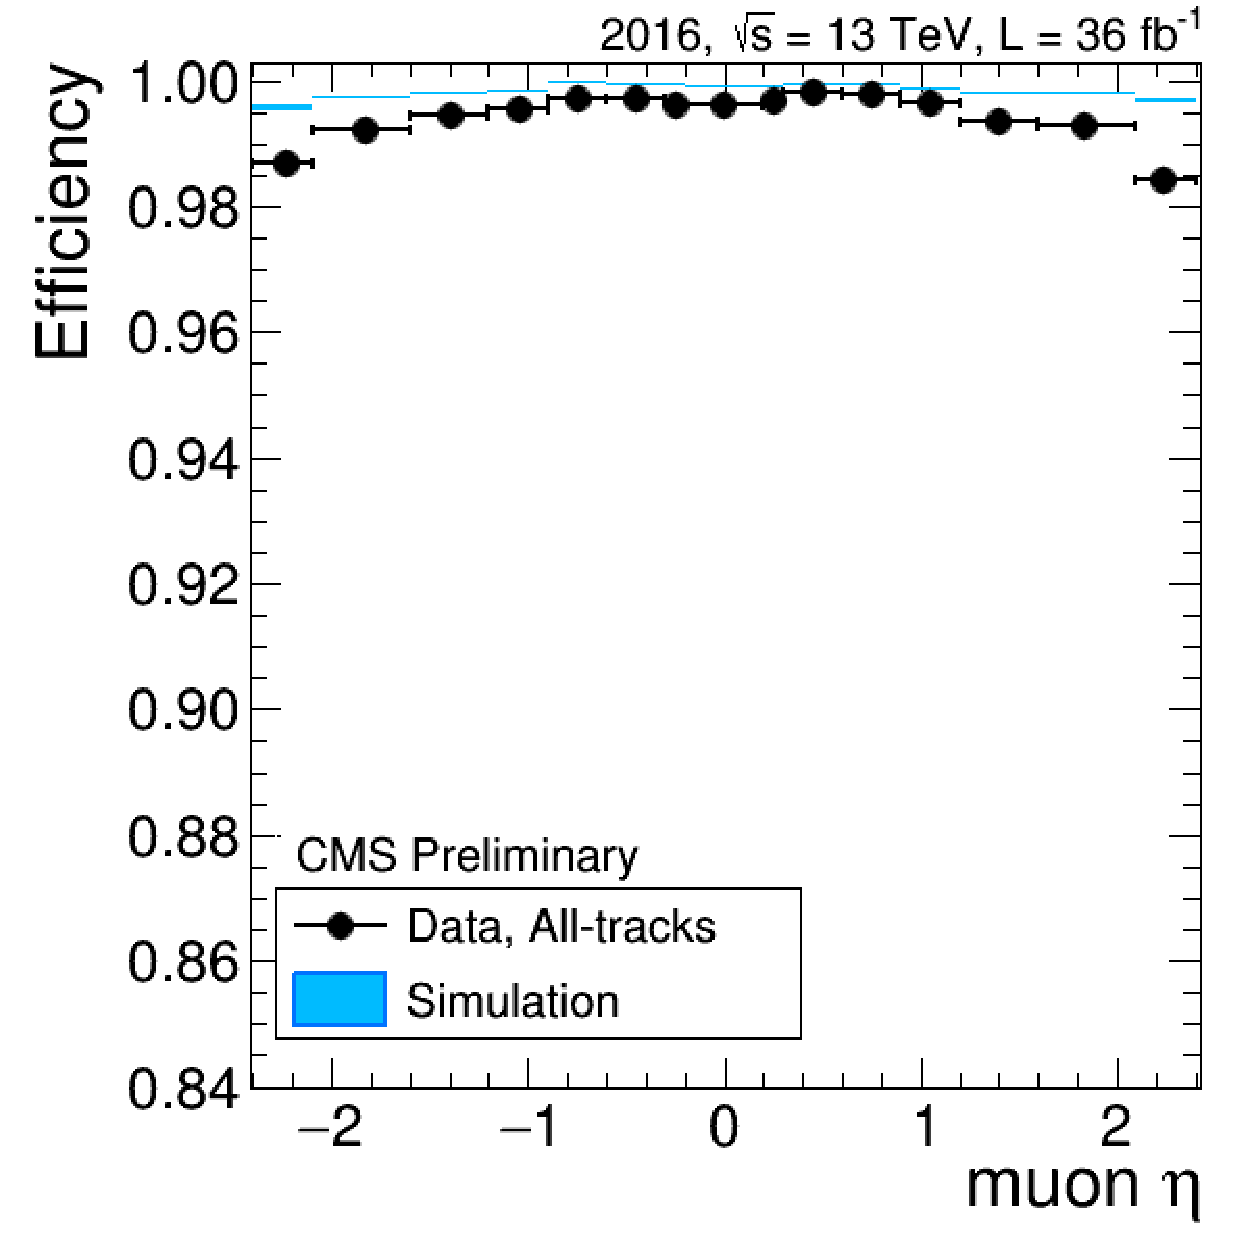
\includegraphics[width=3in]{Figures/Muons/trackingEffptg10.pdf}
\caption{}
\end{subfigure}
    \caption{Tracking efficiency in data and simulation as a function of $\eta$ for muon $\pt < 10\ \GeV$(a) and $\pt > 10\ \GeV$(b) with ReReco data.}
    \label{fig:MuonIDEff_4}
\end{figure}

%\begin{figure}[htbp]
%  \begin{center}
%    \subfigure[]{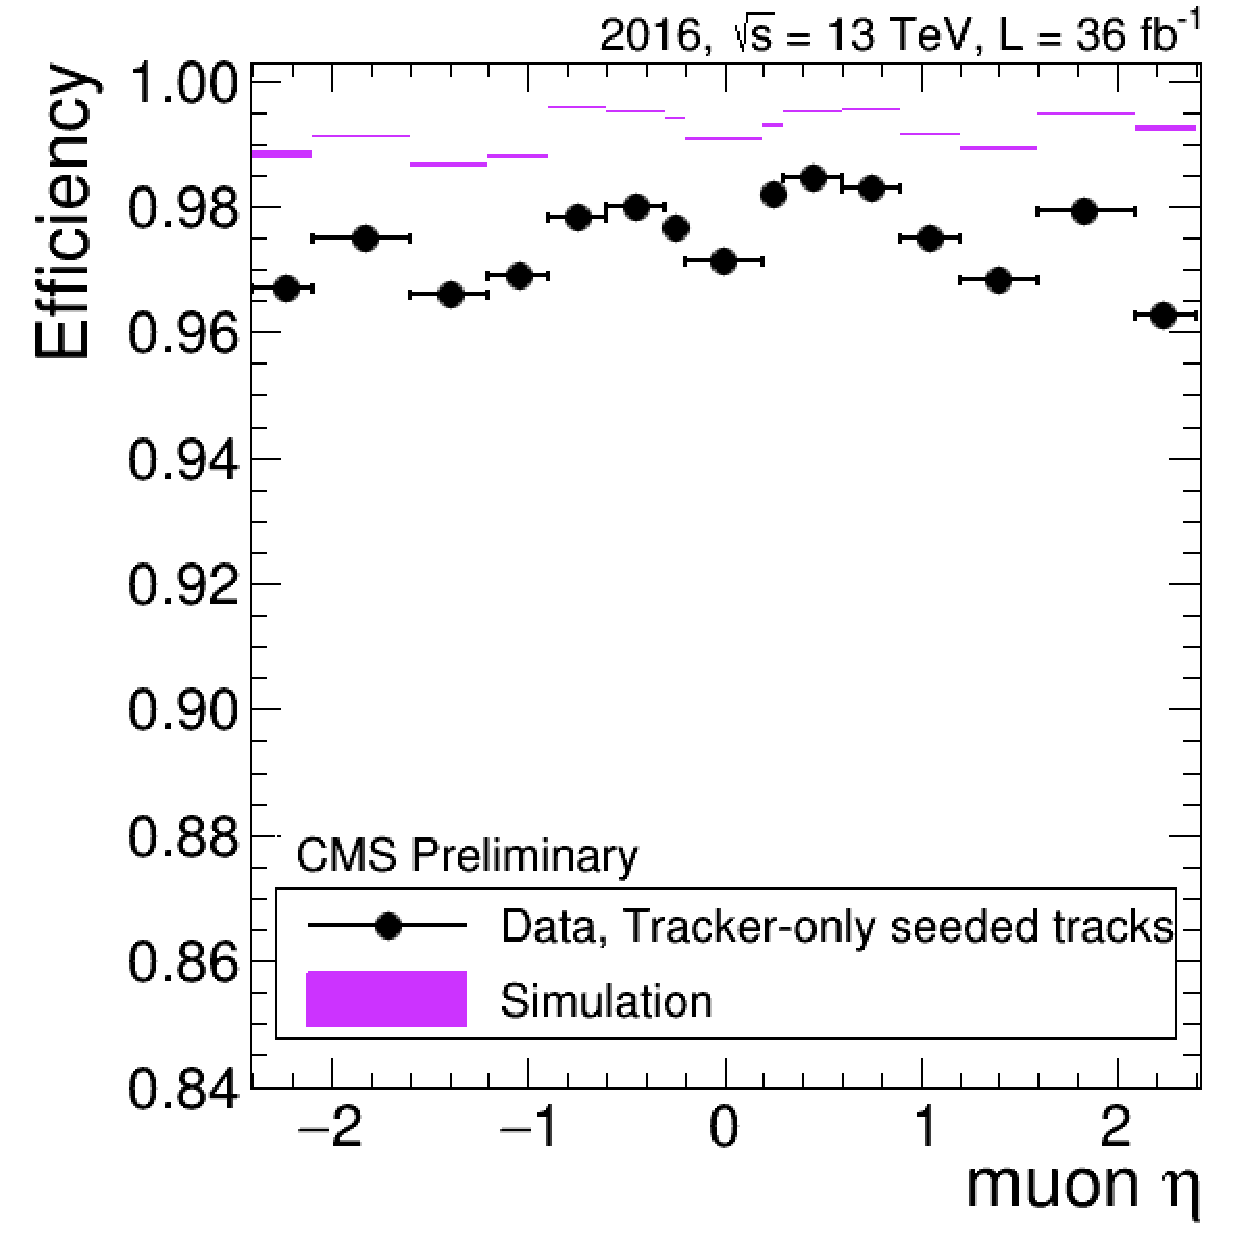
\includegraphics[width=0.42\textwidth]{Figures/Muons/trackingEffptl10.pdf}}
%    \subfigure[]{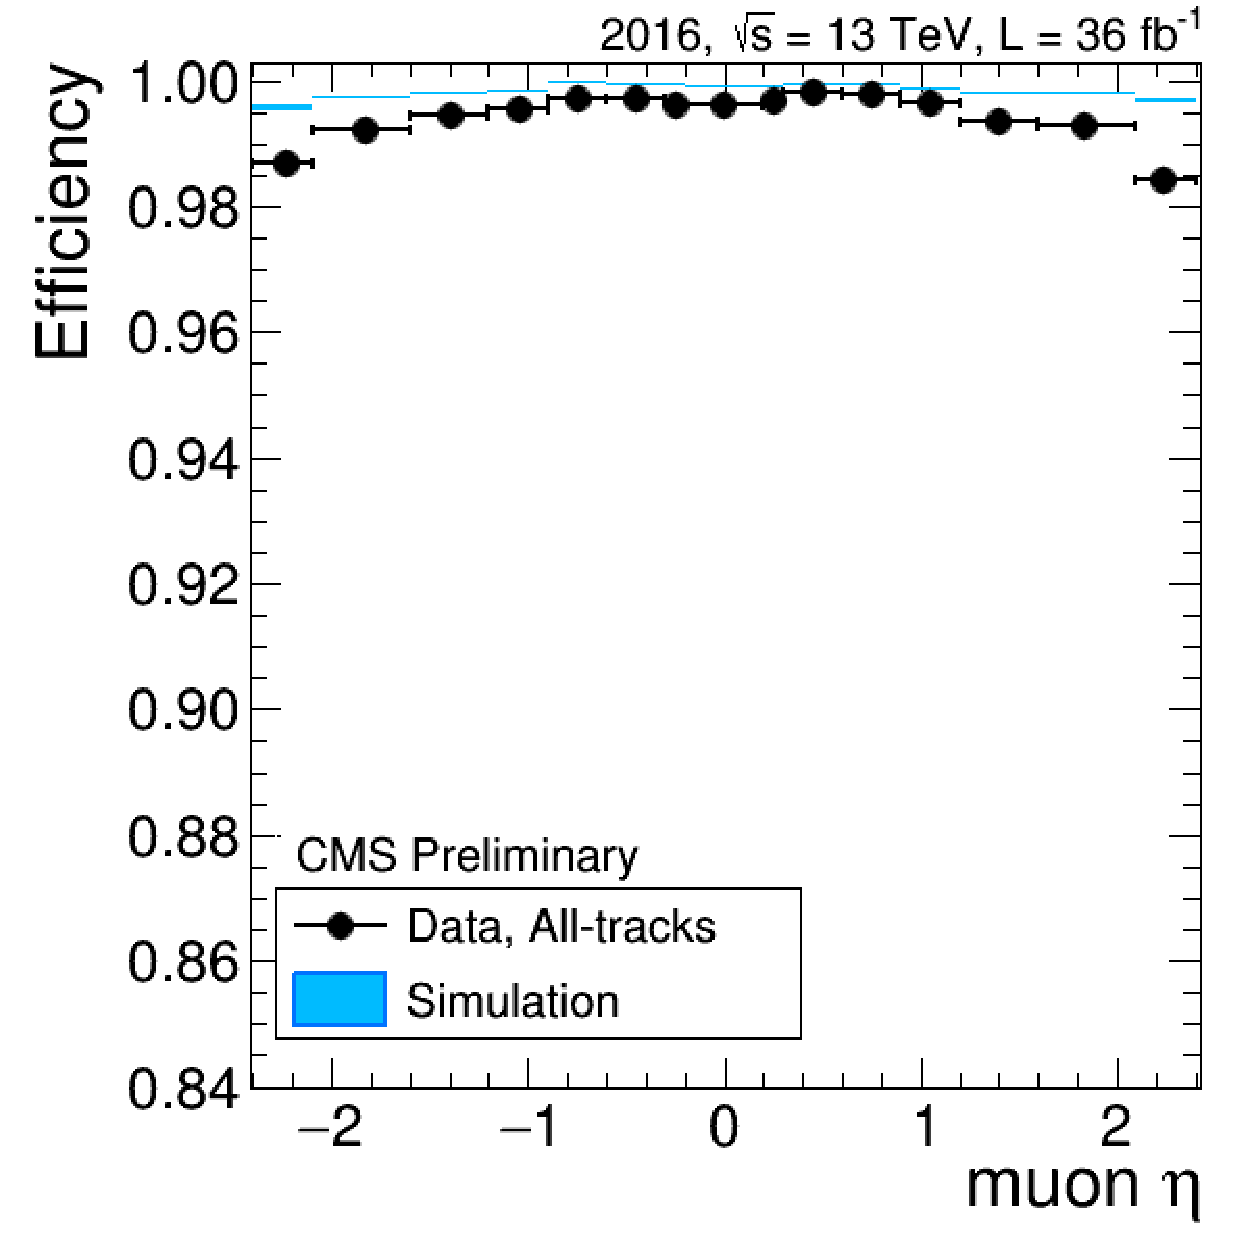
\includegraphics[width=0.42\textwidth]{Figures/Muons/trackingEffptg10.pdf}}
%    \caption{Tracking efficiency in data and simulation as a function of $\eta$ for muon $\pt < 10\GeV$(left) and $\pt > 10\GeV$(right) with ReReco data.}
%    \label{fig:MuonIDEff_4}
%\end{center}
%\end{figure}

\subsubsection{Overall results}
The product of all the data-to-MC scale factors for muon tracking, reconstruction, identification, impact parameter, and isolation requirements is shown in Figure~\ref{fig:MuonIDEff_5}. 
%The overall correction is about $-1\%$ or less for most \pt and $\eta$ values, increasing to about $-2\%$ in for muons below $10\GeV$ or with $|\eta|>2$.

\begin{figure}[tbh]
\centering
\begin{subfigure}{0.45\textwidth}
\centering
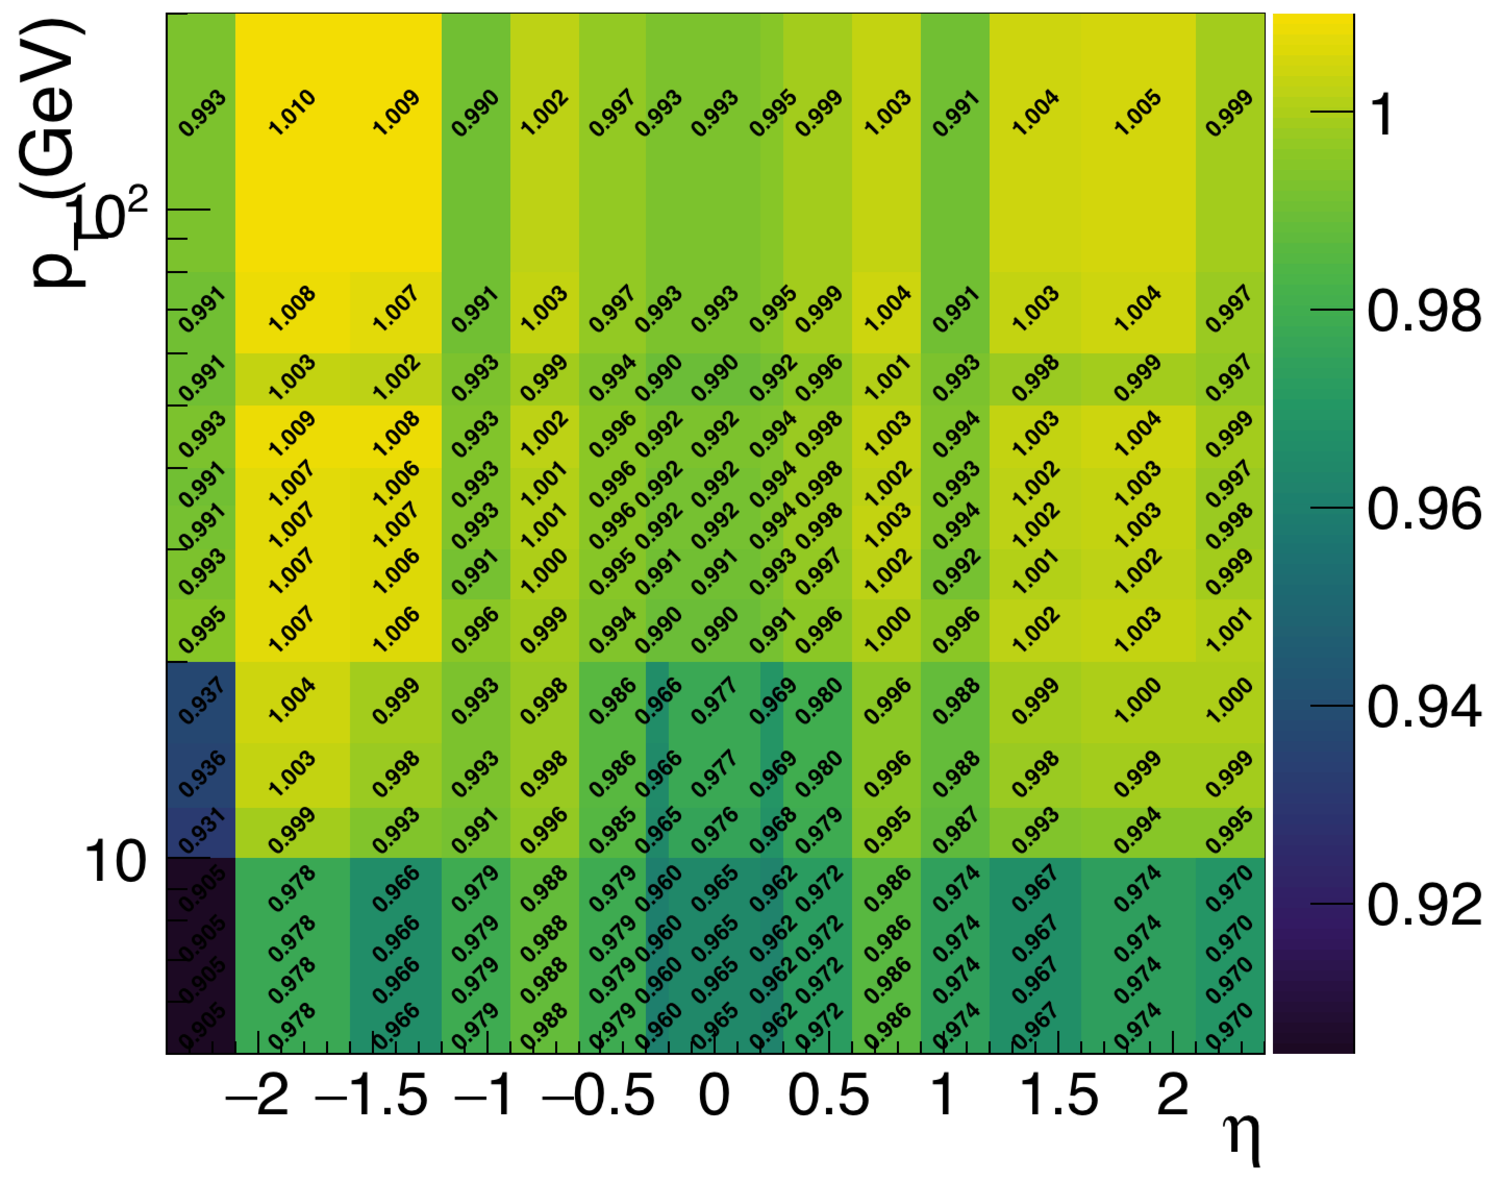
\includegraphics[width=3in]{Figures/Muons/mu_sf.pdf}
\caption{}
\end{subfigure}
\begin{subfigure}{0.45\textwidth}
\centering
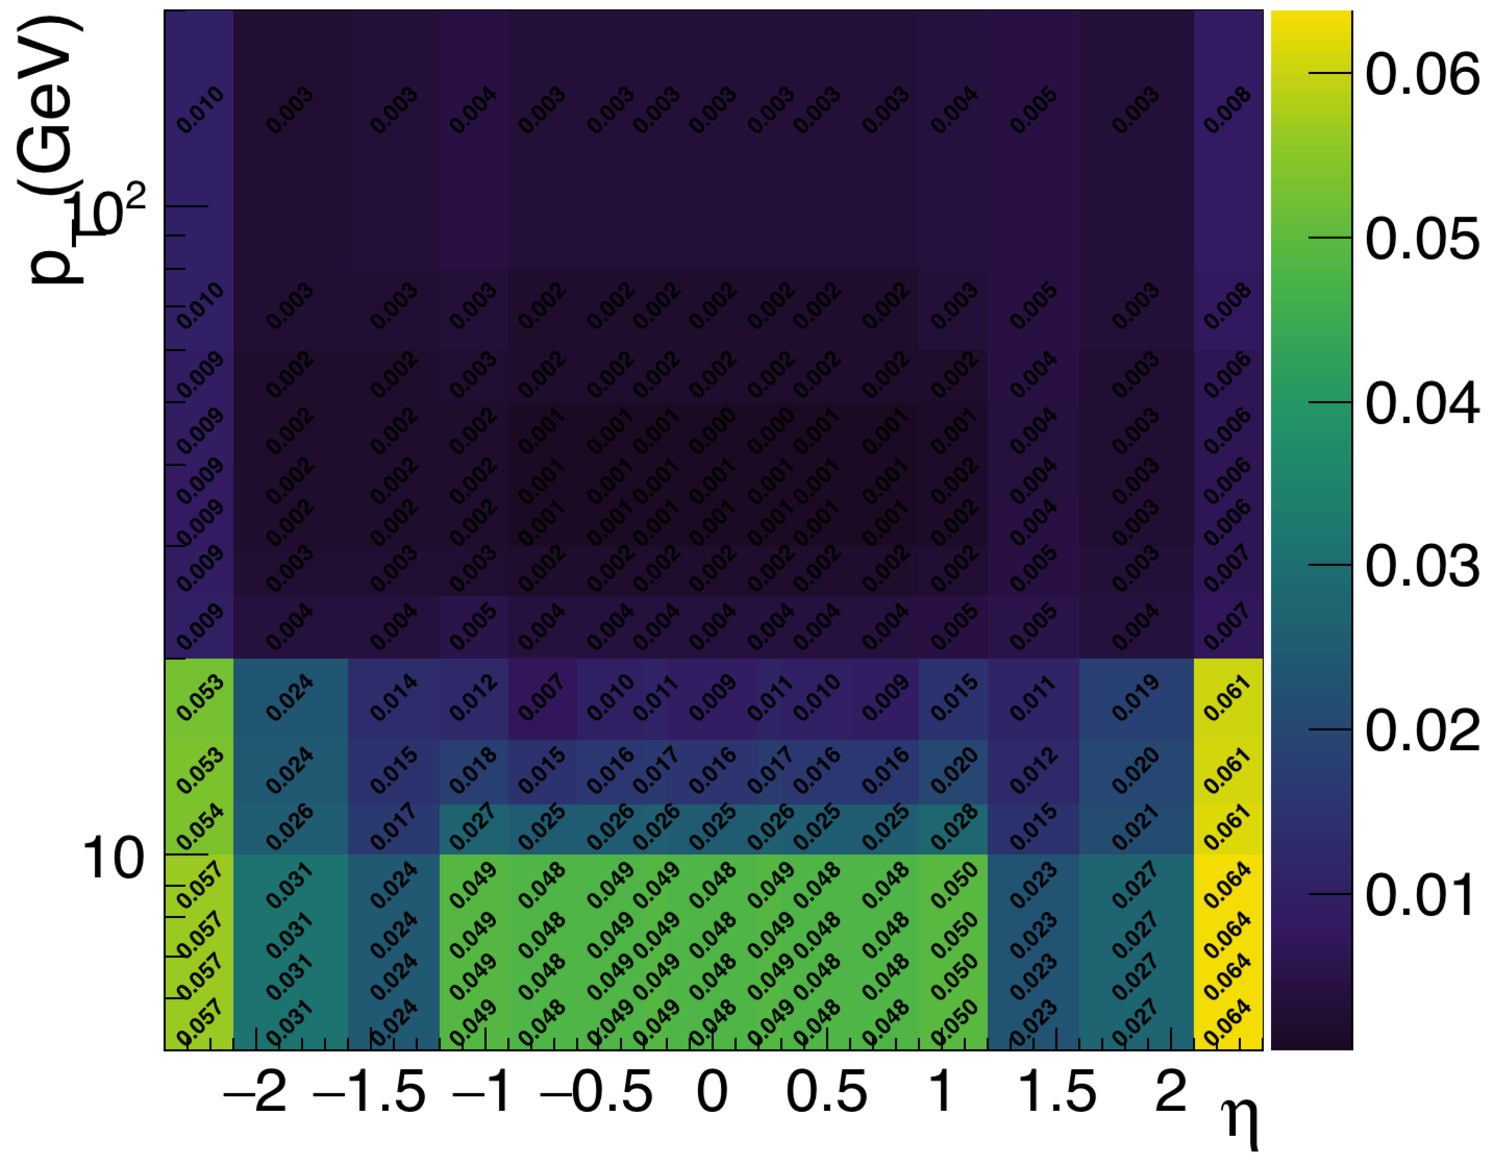
\includegraphics[width=3in]{Figures/Muons/mu_sf_unc.pdf}
\caption{}
\end{subfigure}
    \caption{(a) Overall data to simulation scale factors for muons, as function of $\pt$ and $\eta$. (b) Uncertainties on  data to simulation scale factors for muons, as function of $\pt$ and $\eta$.}
    \label{fig:MuonIDEff_5}
\end{figure}

%\begin{figure}[htbp]
%  \begin{center}
%    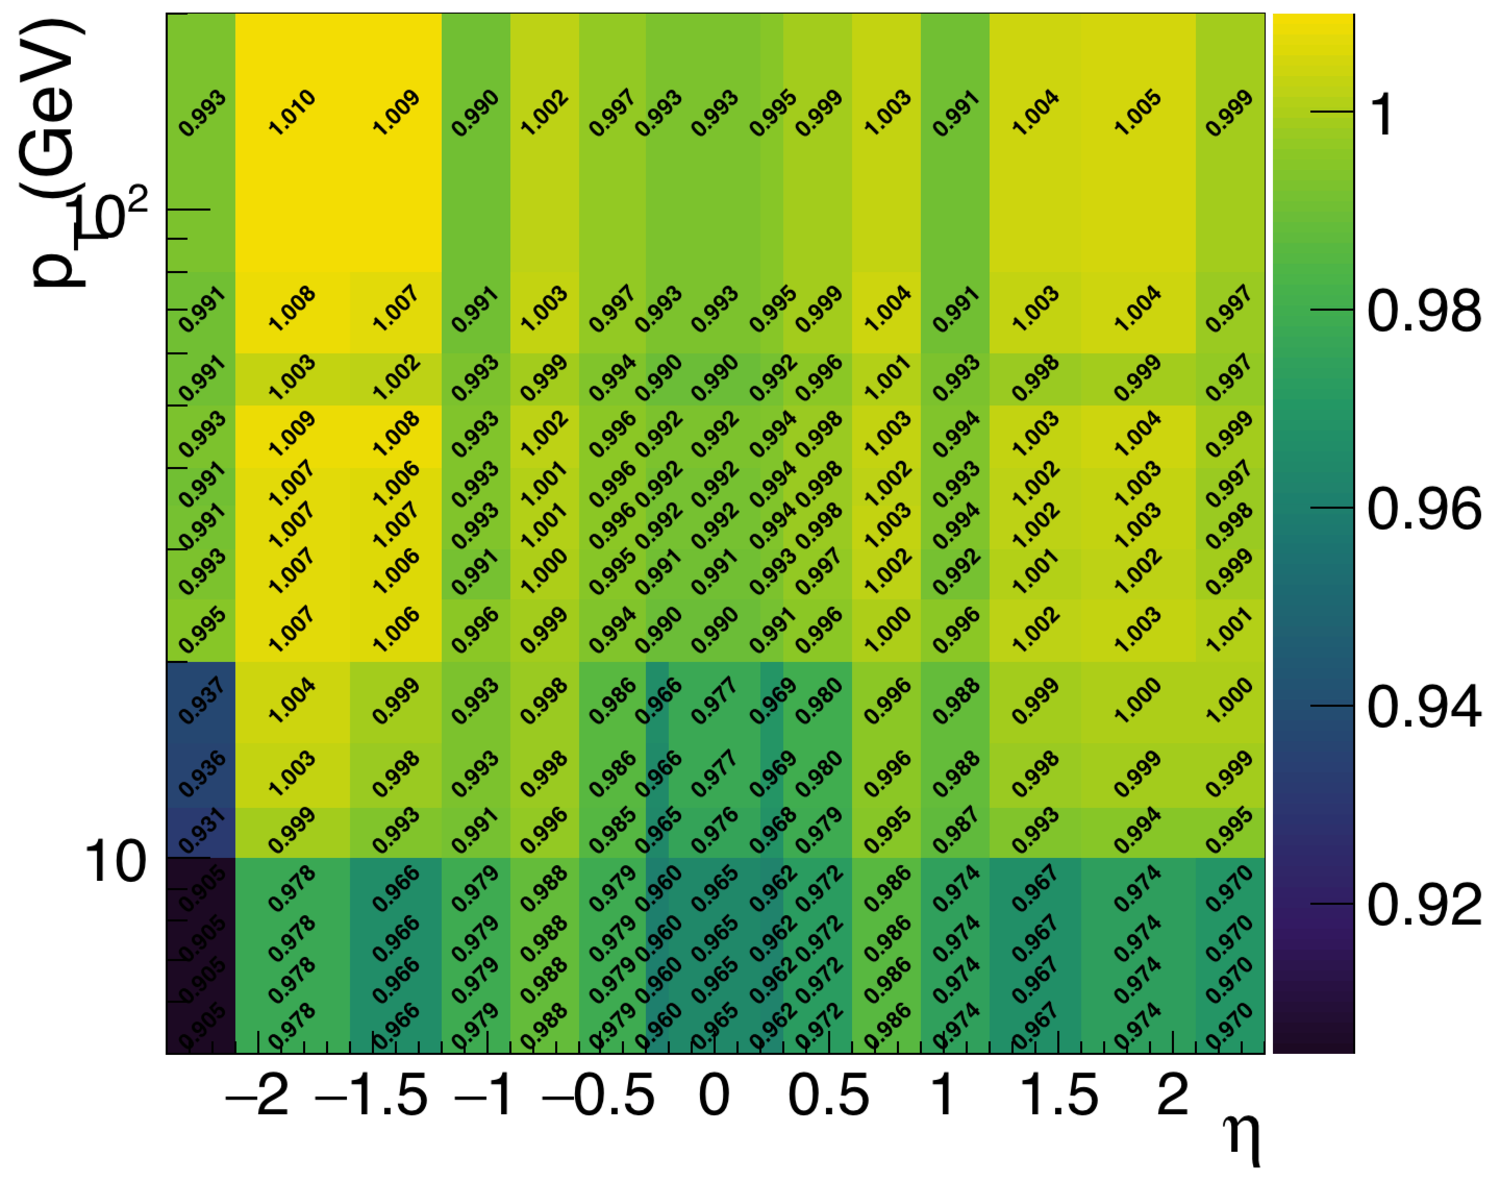
\includegraphics[width=0.45\textwidth]{Figures/Muons/mu_sf.pdf}
%    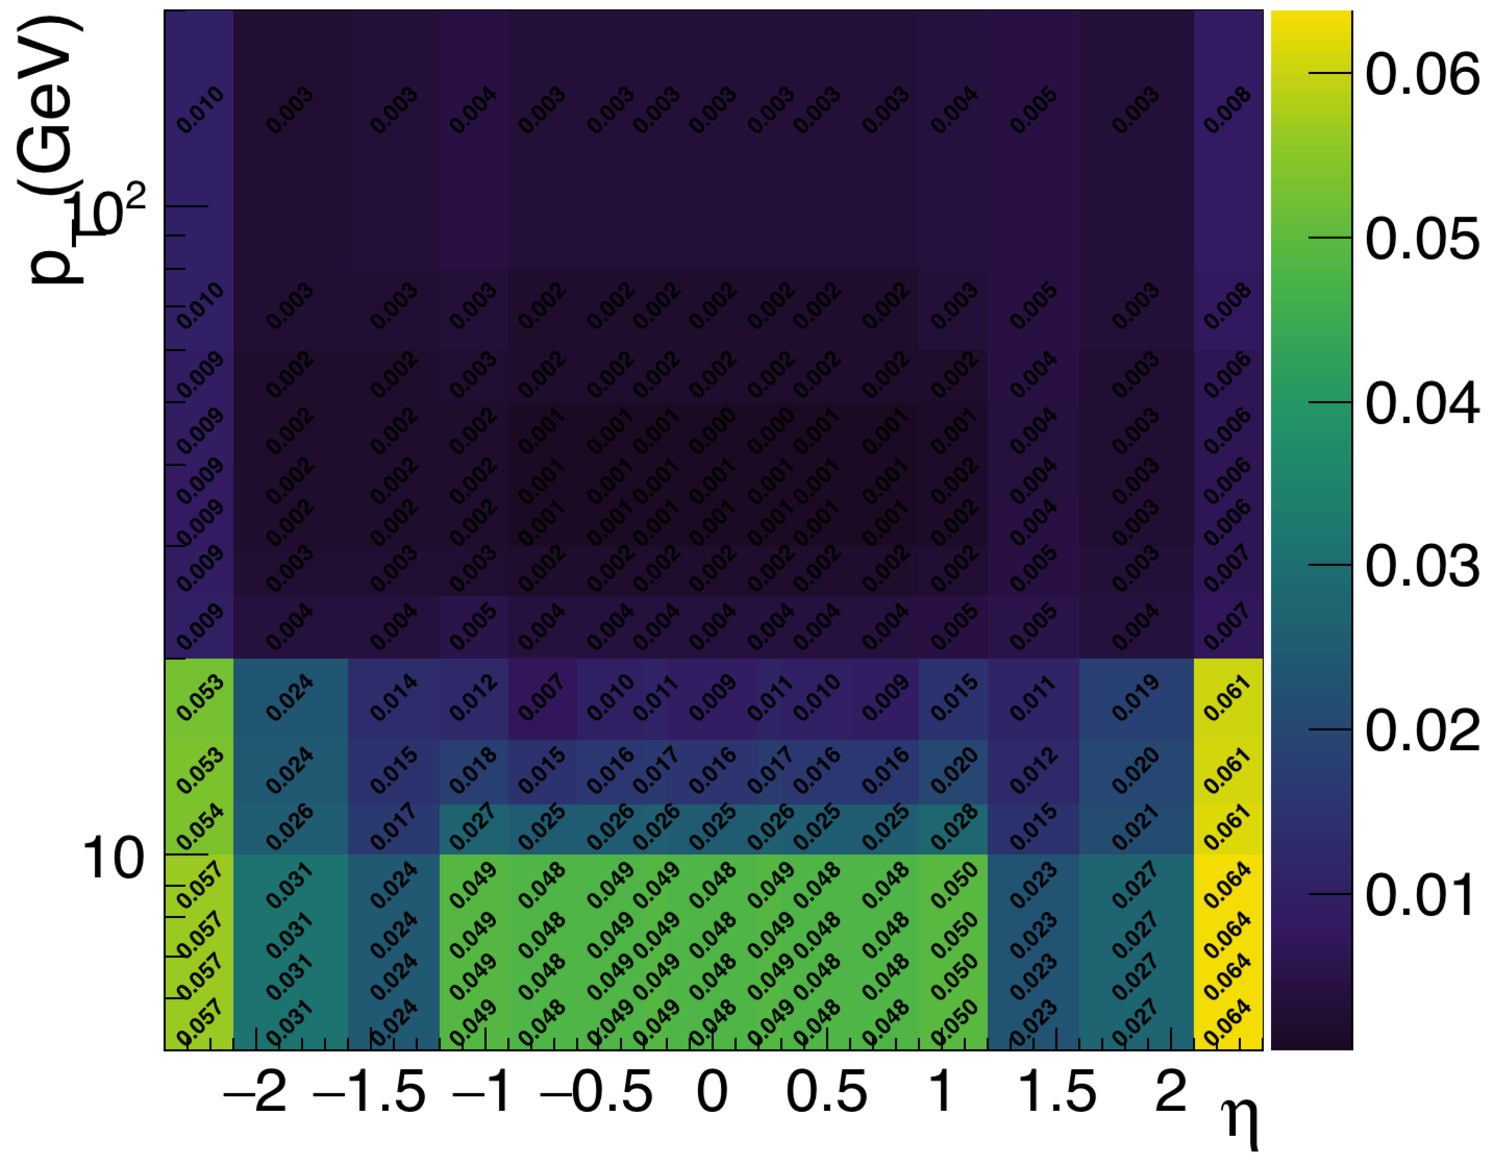
\includegraphics[width=0.45\textwidth]{Figures/Muons/mu_sf_unc.pdf}
%    \caption{Left: Overall data to simulation scale factors for muons, as function of \pt and $\eta$. Right: Uncertainties on  data to simulation scale factors for muons, as function of \pt and $\eta$.}
%    \label{fig:MuonIDEff_5}
%\end{center}
%\end{figure}


\section{Photons for FSR recovery}
\label{sec:FSRphotons}

The FSR recovery algorithm was considerably simplified with respect to what was done in Run 1, while maintaining similar performance. 
The selection of FSR photons is now only done per-lepton and no longer depends on any $Z$ mass criterion, simplifying the subsequent $ZZ$ candidate building and selection. for the association of photons with leptons, the rectangular cuts on $\Delta R(\gamma,l)$ and $E_{T,\gamma}$  have been replaced by a cut on $\Delta R(\gamma,l)/E_{T,\gamma}^{2}$.

Starting from the collection of PF photons provided by the PF algorithm, the selection of photons and their association to a lepton proceeds as follows \cite{AN-15-277, AN-16-217}:

\begin{enumerate}
\item The preselection of PF photons is done by requiring $p_{T,\gamma} > 2~\GeV$, $|\eta^{\gamma}| < 2.4$, and a relative PF isolation $<1.8$. The isolation is computed using a cone of radius $R=0.3$, a threshold of $0.2~\GeV$ on charged hadrons with a veto cone of $0.0001$, and $0.5~\GeV$ on neutral hadrons and photons with a veto cone of $0.01$, also including the contribution from pileup vertices (with the same radius and threshold as per charged isolation) .
\item Supercluster veto: all PF photons that match with any electron passing both the loose ID and SIP cuts are removed. The matching is peformed by directly associating the two PF candidates.
\item Photons are associated to the closest lepton in the event among all those that pass both the loose ID and SIP cuts.
\item Photons that fail the cuts $\Delta R(\gamma,l)/E_{T,\gamma}^2 < 0.012$, and $\Delta R(\gamma,l)<0.5$ are discarded.
\item If more than one photon is associated to the same lepton, the lowest-$\Delta R(\gamma,l)/E_{T,\gamma}^2$ is selected.
\item For each FSR photon that was selected, photons from the isolation sum of all the leptons in the event that pass both the loose ID and SIP cuts are excluded. This concerns the photons that are in the isolation cone and outside the isolation veto of said leptons ($\Delta R < 0.4$ AND $\Delta R > 0.01$ for muons and $\Delta R < 0.4$ AND ($\eta^{\text{SC}} < 1.479$ OR $\Delta R > 0.08$) for electrons).
\end{enumerate}

\section{Jets}
\label{sec:jets}

VBF and other $H$ production mechanisms normally have different jet kinematics. 
Therefore, jets can be used to categorize events based on the production mechanisms.

\subsubsection{Jet identification}

Jets are reconstructed by using the anti-$k_T$ clustering algorithm out of PF candidates, with a distance parameter $R = 0.4$, 
after rejecting the charged hadrons that are associated to a pileup primary vertex.

To reduce instrumental background, the loose working point jet ID suggested by the JetMET Physics Object Group is applied. 
In this analysis, the jets are required to be within $|\eta| < 4.7$ area and have a transverse momentum above 30 $\GeV$. 
In addition, the jets are cleaned from any of the tight leptons (passing the SIP and isolation cut computed after FSR correction) 
and FSR photons by a separation criterion: $\Delta R(\text{jet,lepton/photon}) > 0.4$.


\subsubsection{Jet energy corrections}

The calorimeter response to particles is not linear,
and it is not straightforward to translate the measured jet energy
to the true particle or parton energy; therefore, jet energy corrections (JECs) are needed.
In this analysis, standard jet energy corrections are applied to the reconstructed jets,
which consist of L1 Pileup, L2 Relative Jet Correction,
L3 Absolute Jet Correction for both MC samples and data,
and also residual calibration for data.

% Figure~\ref{fig:jets} shows the comparisoin between data and MC for the leading jet in Z events with exactly one jet,
% where a selection $\Delta\phi(Z,{\rm jet})>2.5$ has been applied.

% \begin{figure}[!h]
% \centering
% \includegraphics[width=0.49\linewidth]{Figures/Jets/Histo_etaj1_2e_dataeff.pdf}
% \includegraphics[width=0.49\linewidth]{Figures/Jets/Histo_etaj1_2mu_dataeff.pdf}
% \caption{Comparison between data and MC for jet $\eta$ in Z + 1 jet events. \label{fig:jets}}
% \end{figure}


\subsubsection{B-tagging}

For categorization purposes, whether or not a jet is a b-jet needs to be distinguished.
The Combined Secondary Vertex (CSV) algorithm is used as the b-tagging algorithm.
It combines information about impact parameter significance,
the secondary vertex and jet kinematics.
The variables are combined using a likelihood ratio technique to compute the b-tag discriminator.
In this analysis, a jet is considered to be b-tagged if it passes the \emph{CSVv2M} working point,
i.e. if its pfCombinedInclusiveSecondaryVertexV2BJetTags discriminator is greater than 0.8484~\cite{btagReferenceEffsRun2}.

Data-to-MC scale factors for b-tagging efficiency are provided for this working point for the full dataset as a function of jet $\pt$, $\eta$, and flavor.
They are applied to simulated jets by downgrading (upgrading) the b-tagging status of a fraction of the b-tagged (untagged) jets that have a scale factor smaller (larger) than one.

\section{MET}

The missing transverse energy, $E_{\rm{T}}^{\rm{MISS}}$ or MET, of an event is defined as the magnitude of the imbalance of momentum in the plane transverse to the beam line. Since momentum is conserved in this plane, any imbalance in momentum is attributed to particles escaping the detector without interacting with the detector material, such as neutrinos or hypothetical dark matter candidates. Raw MET or particle flow MET (PFMET) is defined as the magnitude of the negative vectorial sum of the transverse momentum of all reconstructed particle flow candidates, or

\begin{equation}
\overrightarrow{E}_{\rm{T}}^{\rm{MISS}} = - \sum_{i \in \rm{all}} \overrightarrow{p}_{\rm{T},\ i}
\end{equation}

The vector quantity that is the negative sum of reconstructed particle momenta is sometimes called the missing transverse momentum, although this term is used interchangably with its magnitude, the MET. 

An alternative definition of the MET, called the type-1 corrected MET, takes into account the jet energy corrections (JEC), correcting for mismeasurement of MET due to detector inefficiencies and non-linear responses in the calorimeters. The type-1 corrected MET definition is given by:

\begin{equation}
\label{eq:t1met}
\overrightarrow{E}_{\rm{T\ Type-1}}^{\rm{MISS}} = - \sum_{jet} \overrightarrow{p}_{\rm{T},\ jet}^{\rm{JEC}} - \sum_{i \in \rm{uncl.}} \overrightarrow{p}_{\rm{T},\ i}
\end{equation}
where the total contribution has been split into contributions from jets (first term) and contributions from unclustered objects (second term). The transverse momenta of jets in the first term is then replaced with the JEC transverse momenta.

Systematic uncertainties related to modeling real MET are obtained by varying the JEC and jet energy resolution (JER) and measuring the propogation of these variations to the MET uncertainty. These measurements are described in greater detail in Section~\ref{sec:metsyst}.

\subsubsection{MET filters}

Due to detector and instrumental noise, several filters are applied to veto noisy events \cite{mettwiki}:
HBHENoiseFilter,
HBHENoiseIsoFilter,
EcalDeadCellTriggerPrimitiveFilter, 
goodVertices, 
eeBadScFilter, 
globalTightHalo2016Filter, 
BadPFMuonFilter, and
BadChargedCandidateFilter.

The first two filters remove noisy events from the HCAL, where the HBHE scintillator produce anamolous signals with pulse shapes and pixel multiplicities discrepant from those from a clean signal. The EcalDeadCellTriggerPrimitiveFilter removes events with down ECAL data links, comparing the sum of energy deposited in each cell of a supercluster to the trigger primitive saturation energy. The goodVertices filter removes events with noisy vertex reconstruction from pileup effects. The eeBadScFilter removes events with noisy ECAL end cap superclusters. Tje globalTightHalo2016Filter filter removes events with enhanced MET from beam-halo particles which are in time with the beam. The last two filters remove events with mis-reconstructed muon and charged hadron particle flow candidates.

\subsubsection{Fake MET modeling}\label{sec:fakemet}

Figure~\ref{fig:pfmet_m4lblinded} shows a discrepancy between data and MC in the high-$E_{\rm{T}}^{\rm{MISS}}$ tail. These events typically contain a high $p_T$ object either back-to-back or collinear with the $E_{\rm{T}}^{\rm{MISS}}$, pointing to artificially high $E_{\rm{T}}^{\rm{MISS}}$ from mismeasurement of the object. These events are identified and removed by studying distributions of the transverse angular difference between the MET and various objects in the event \cite{CMS-AN-15-203}.

\begin{figure}[tbh]
\centering
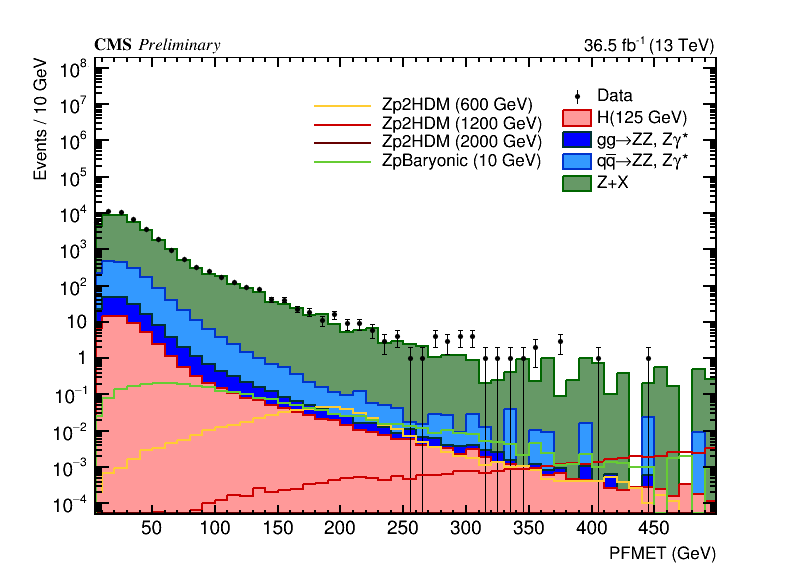
\includegraphics[width=5in]{figures/hist_hPFMET_3.png}
\caption{Missing transverse energy (MET) after the first $Z$ selection step before removal of fake MET.}
\label{fig:pfmet_m4lblinded}
\end{figure}

The following variables are studied in order to understand how to remove events with fake MET from data: (1) $max|\Delta\phi(jet, E_{\rm{T}}^{\rm{MISS}})|$ with the maximum taken over selected jets, Figure~\ref{fig:maxdeltaphijmet} and (2) $min|\Delta\phi(jet, E_{\rm{T}}^{\rm{MISS}})|$ with the minimum taken over selected jets, Figure~\ref{fig:mindeltaphijmet}
The maximum variable is to check for the occurance of objects with mismeasured energy back-to-back with the MET, while the minimum variable is to check for jets with mismeasured energy collinear with the MET.

\begin{figure}[tbh]
\centering
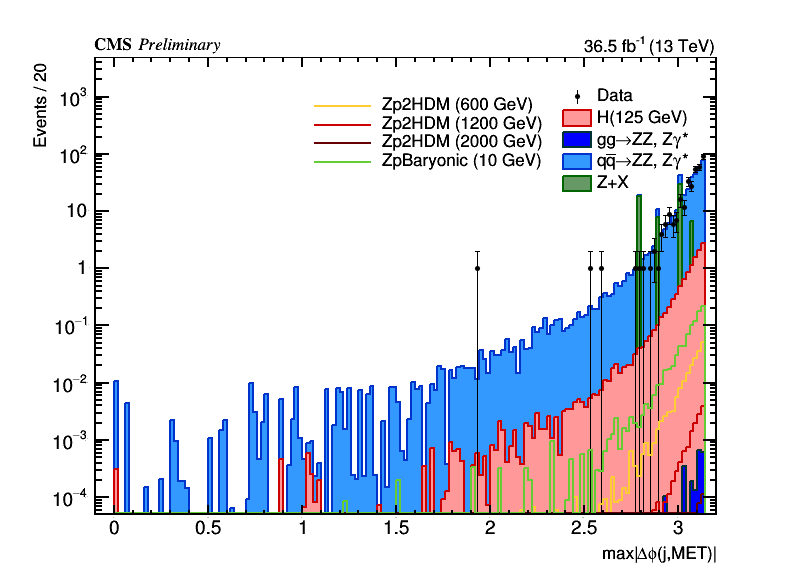
\includegraphics[width=5in]{figures/hist_hDPHI_MAX_JET_MET_8.png}
\caption{Maximum azimuthal angle difference between MET and jets.}
\label{fig:maxdeltaphijmet}
\end{figure}

\begin{figure}[tbh]
\centering
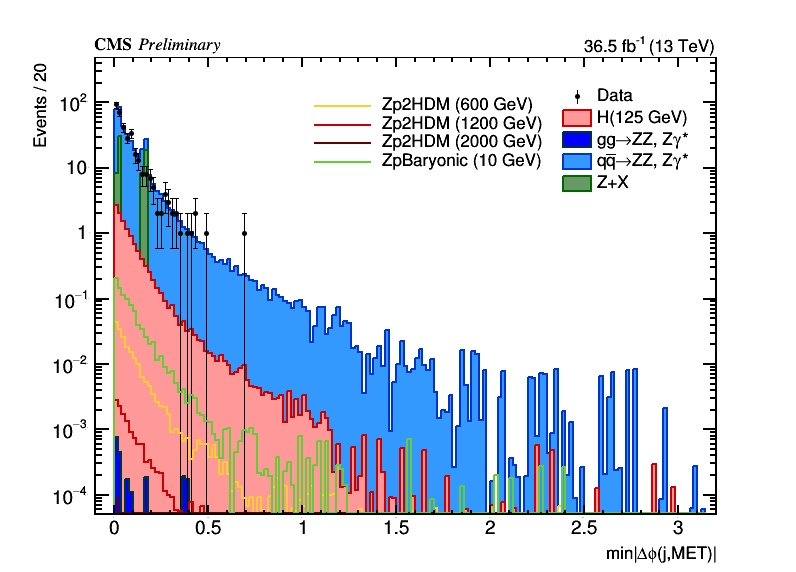
\includegraphics[width=5in]{figures/hist_hDPHI_MIN_JET_MET_8.png}
\caption{Minimum azimuthal angle difference between MET and jets.}
\label{fig:mindeltaphijmet}
\end{figure}

For jets with a high transverse momentum, $>50\ \GeV$, it is required that $max|\Delta\phi(jet, E_{\rm{T}}^{\rm{MISS}})|<2.7$ and $min|\Delta\phi(jet, E_{\rm{T}}^{\rm{MISS}})|>0.5$ to exclude events with large MET from mismeasurment of jet energies. These cuts are based on the Run 1 SM analysis selection, chosen to balance the small loss in signal efficiency with the increased systematic uncertainty from mismodeling of the MET in background MC simulations (described in Section~\ref{sec:metsyst}).

